\documentclass[numerate]{cheatsheet}
\usepackage{blindtext}
\usepackage{multicol}
\usepackage{tabularx}
\usepackage{empheq}
\usepackage{makecell}
\usepackage{xcolor}
\usepackage{scalerel}
\usepackage{amsmath}
\usepackage{graphicx}
\usepackage{wrapfig}
\usepackage{wasysym}
\usepackage{amssymb}
\usepackage{color,soul}
\usepackage{colortbl}
\usepackage{multirow}
\usepackage{bigstrut}
\usepackage[center]{}

\graphicspath{ {./Dokumente/ZF_nischmidt_MAE/Pictures} }


\doctitle{Zusammenfassung \\Maschinenkonstruktion}
\author{Nina Schmidt - nischmidt$@$ethz.ch}


\begin{document}

\renewcommand{\multirowsetup}{\centering} %to align center inside the table
\setlength{\tabcolsep}{4pt}
%New command
\newcommand{\cbreak}{%
    \vfill\null\columnbreak%
}

%New command
\makeatletter
\newcommand{\pushright}[1]{\ifmeasuring@#1\else\omit\hfill$\displaystyle#1$\fi\ignorespaces}
\newcommand{\pushleft}[1]{\ifmeasuring@#1\else\omit$\displaystyle#1$\hfill\fi\ignorespaces}
\makeatother


\section{Dimensionierung \hfill ME}
    \begin{minipage}{0.58\linewidth}
    \begin{center}
        \begin{footnotesize}  
        \mathbox{
            S_F = \frac{R}{B} = \frac{\text{Belastbarkeit}}{\text{Beanspruchung}}
        }
        \mathbox{
            \sigma = \frac{F}{A}
        }
        \end{footnotesize}
    \end{center}
\end{minipage}
\begin{minipage}{0.4\linewidth}
    \begin{center}
        \begin{scriptsize}
            \begin{align*}
                &S_F = \text{Sicherheitsfakor;}
                \\ &R = R_m \text{bzw.} R_{p0.2}
                \\~\\ &\textbf{Beanspruchungsarten:}
                \\ &\text{Mechanik (Statik \& Mechanik)}
                \\ &\text{Umwelteinflüsse (Feuchtigkeit)}
                \\ &\text{Belastungsdauer}
                \\ &\text{Belastungshöhe (Intensität)}
            \end{align*}
        \end{scriptsize}
    \end{center}
\end{minipage}

\section{Zahnräder und Zahnradgetriebe \hfill ME}
    \subsection{Übersetzung \hfill ME}
\begin{minipage}{0.68\linewidth}
    \begin{center}
        \begin{footnotesize}
        \begin{empheq}[box=\fbox]{align*}
            &i = \frac{\omega_{1(\text{an})}}{\omega_{2(\text{ab})}} = \frac{n_{1(\text{an})}}{n_{2(\text{ab})}} = \frac{d_{tk{2(\text{ab})}}}{d_{tk{1(\text{an})}}}
            \\ & = \frac{M_{2(\text{ab})}}{\eta M_{1(\text{an})}} = \frac{z_{2(\text{ab})}}{z_{1(\text{an})}}
        \end{empheq}
        \vspace{-2mm}
        \mathbox{
            i_{\text{ges}} = i_{1,2} \cdot i_{3,4} \cdot i_{5,6} = \frac{z_2 \cdot z_4 \cdot z_6}{z_1 \cdot z_3 \cdot z_5}
        }
        \vspace{-3mm}
        \mathbox{
            d_{tk} = \frac{U_{tk}}{\pi} = z_x \cdot \frac{p}{\pi} = z_x \cdot m
        }
        \vspace{-3mm}
        \mathbox{
            d_{a} = d_{tk} + 2 \cdot m
        }
        \vspace{-3mm}
        \mathbox{
            Z_g = \frac{2}{\sin(\alpha)^2}        
            }
            \vspace{-3mm}
            \mathbox{
                N_2 = \frac{r_1}{r_2} \cdot n_1 \; M_2 = \frac{r_2}{r_1} \cdot M_1
            }
        \end{footnotesize}
    \end{center}
\end{minipage}
\begin{minipage}{0.31\linewidth}
    \begin{center}
        \begin{scriptsize}
        \begin{align*}
            &\text{$i$ = Übersetzung};
            \\ &\text{$i < 1$: Abtr. schneller;}
            \\ &\text{$i > 1$: Abtr. langsamer;}
            \\ &\text{$\omega_x$ = Winkelgeschw.};
            \\&\text{$n_x$ = Drehzahl};
            \\&\text{$d_{tk}$ = Teilkreisdurchm.;}
            \\&\text{$M_x$ = Drehmoment;}
            \\&\text{$\eta$ = Wirkungsgrad;}
            \\&\text{$z_x$ = Zähnezahl};
            \\ &\text{$U_{tk}$ = Teilkreisumfang};
            \\ &\text{$p$ = Teilung};
            \\ &\text{$m$ = Modul \textcolor{Red}{= const.}};
            \\ &\text{$d_a$ = Aussendurchm.};
            \\ &P_{ab/an} = \text{Leistung};
            \\ &Z_g = \text{Grenzzähnezahl}
        \end{align*}
        \end{scriptsize}
    \end{center}
\end{minipage}

\vspace{2mm}

\center{\footnotesize{Weitere Beziehungen:}}
\begin{footnotesize}
    \vspace{-1mm}\mathbox{
    m = \frac{p}{\pi} \; \mid \; \omega_x = 2\pi n_x \; \mid \; \eta = \frac{P_{ab}}{P_{an}} = \frac{M_2n_2}{M_1n_1} = \frac{M_2}{M_1i} < 1
}
\end{footnotesize}
\begin{minipage}{0.58\linewidth}
    \begin{center}
        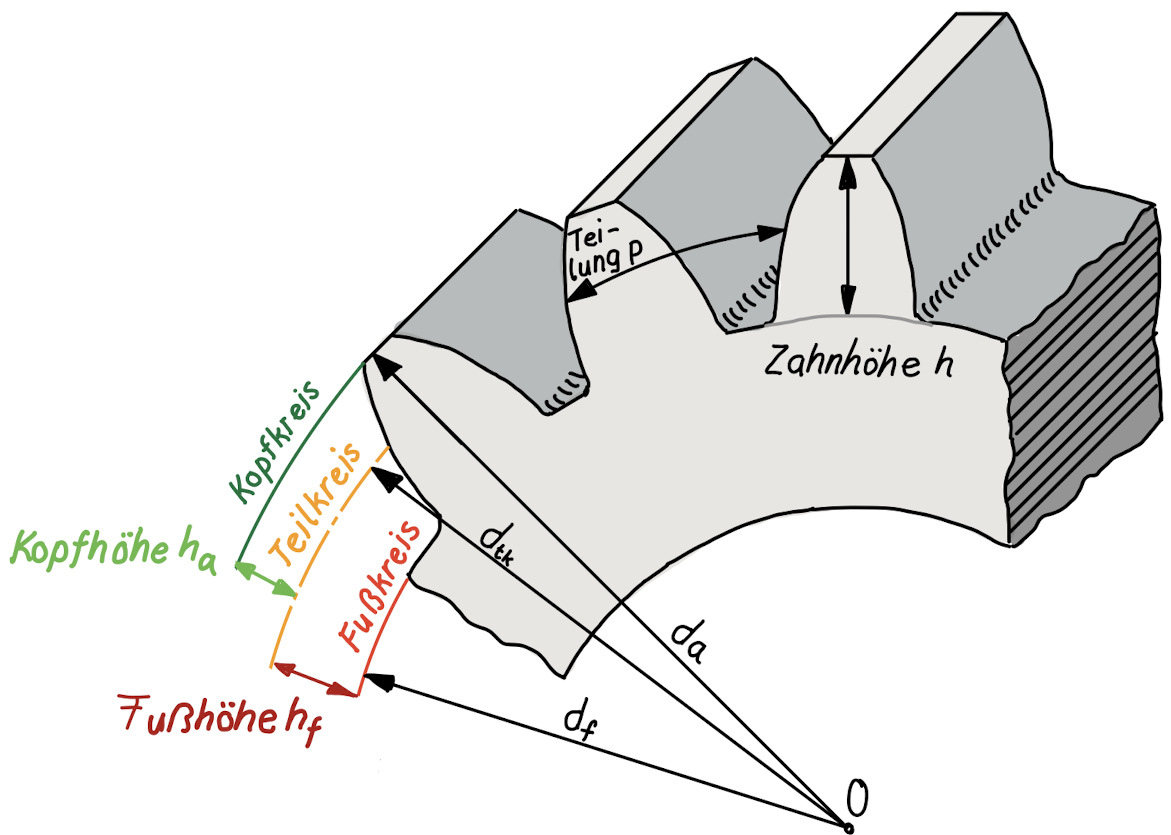
\includegraphics[width = 1.1\linewidth]{src/images/MAEIP_Zahnrad}
    \end{center}
\end{minipage}
\begin{minipage}{0.35\linewidth}
    \begin{center}
        \begin{scriptsize}
            \begin{align*}
                d_f &= \text{Fusskreis-} \varnothing
                \\d_{tk} &= \text{Teilkreis-} \varnothing
                \\d_a &= \text{Kopfkreis-} \varnothing
                \\ p&= \text{Teilung}
                \\ h_a &= \text{Zahnkopfhöhe} 
                \\ h_f &= \text{Fusshöhe}
                \\ h &= \text{Zahnhöhe}
             \end{align*}
        \end{scriptsize}    
    \end{center}
\end{minipage}

\begin{footnotesize}
    \begin{empheq}[box=\fbox]{align*}
        h = h_a + h_f \quad \mid \quad h_a = m \quad \mid \quad h_f = 1.1, ..., 1.3 \cdot m
    \end{empheq}
\end{footnotesize}

\subsubsection{Kräfte - geradverzahntes Zahnrad \hfill ME}
\vspace{-1mm}\begin{minipage}{0.4\linewidth}
    \begin{footnotesize}
        \begin{center}
            \mathbox{
                F_{t1} = F_{t2} = \frac{2M_1}{d_1}
            }
        \end{center}
    \end{footnotesize}
\end{minipage}
\begin{minipage}{0.58\linewidth}
    \begin{footnotesize}
        \begin{center}
            \mathbox{
                F_{r1} = F_{r2} = F_{t1} \cdot tan(\alpha)
            }
        \end{center}
    \end{footnotesize}
\end{minipage}

\subsubsection{Achsabstand $a$ \hfill ME}
\vspace{-1mm}
\mathbox{
    a = \frac{d_{tk1}}{2} + \frac{d_{tk2}}{2}
}
\vspace{0.1mm}
    \subsection{Mechanische Leistung $P$ \hfill ME}
\vspace{0.3em}
        \begin{footnotesize}
            \mathbox{
            P = M_x \cdot \omega_x = M_x \cdot 2\pi \cdot n_x
        }
        \mathbox{
            P_{an} = M_1 \cdot 2 \cdot \pi \cdot n_1 \quad \mid \quad P_{ab} = M_2 \cdot 2 \cdot \pi \cdot n_2
        }
        \mathbox{
            1W = \frac{kg \cdot m^2}{s^3} = 1 \frac{J}{s} = \frac{Nm}{s} = 60 \frac{Nm}{min}
        }
        \end{footnotesize}
    \subsection{Schrägverzahnte Stirnräder \hfill ME}
\begin{scriptsize}
    \begin{itemize}
    \item Ermöglicht Verlängerung d. Eingriffsstrecke ($\Delta q$) $\to$ höhere Belastbarkeit \\und ruhigeres Laufverhalten $\to$ teuer
    \end{itemize}
\end{scriptsize}
\vspace{-3mm}
\begin{minipage}{0.58\linewidth}
    \begin{footnotesize}
        \begin{center}
            \begin{empheq}[box=\fbox]{align*}
                \Delta q &= b \cdot tan(\beta)
                \\ &= \frac{p \cdot d_f}{E_A} \cdot K
                \\m_t &= \frac{m_n}{cos(\beta)}
                \\cos(\beta) &= \frac{m_n}{m_t} = \frac{m_n \cdot z}{d_{tk}}
                \\d &= m_t \cdot z
                \\z'_{gt} &= 14 \cdot cos^3(\beta)
            \end{empheq}
        \end{center}
    \end{footnotesize}
\end{minipage}
\begin{minipage}{0.4\linewidth}
    \begin{scriptsize}
            \begin{align*}
                b &= \text{Breite ZR}
                \\m_t &= \text{Stirnmodul}
                \\m_n &= \text{Normalmodul}
                \\z'_{gt} &= \text{Grenzzähnezahl}
                \\p &= \text{Pressung}
                \\ d_f &= \text{Durchmesser Fuge}
                \\ E_A &= \text{E-Modul Nabe}
                \\K &= \text{aus Tabelle}
                \\ &\textbf{Grenzzähnezahl:}
                \\ &\text{Theoretisch:} \; z < 17
                \\ &\text{Praktisch:} \; z < 14
            \end{align*}
    \end{scriptsize}
\end{minipage}

\subsubsection{Kräfte - schrägverzahntes Zahnrad \hfill ME}
\vspace{-1mm}\begin{minipage}{0.4\linewidth}
    \begin{footnotesize}
        \begin{center}
            \mathbox{
                F_{t1} = F_{t2} = \frac{2M_1}{d_1}
            }
        \end{center}
    \end{footnotesize}
\end{minipage}
\begin{minipage}{0.58\linewidth}
    \begin{footnotesize}
        \begin{center}
            \mathbox{
                F_{r1} = F_{r2} = F_{t1} \cdot tan(\alpha)
            }  
            \vspace{-2mm}
            \mathbox{
                F_{a1} = F_{a2} = F_{t1}\cdot tan(\beta)
            }
            \mathbox{
                d = m_t \cdot z \mid m_t = \frac{m_n}{\cos(\beta)}
            }
        \end{center}
    \end{footnotesize}
\end{minipage}
    \subsection{Kegelradpaar \hfill ME}

\begin{minipage}{0.45\linewidth}
        \begin{footnotesize}
            \begin{center}
            \begin{empheq}[box=\fbox]{align*}
                i &= \left\{...\right\} = \frac{d_{m2}}{d_{m1}}\\ &= \frac{d_{e2}}{d_{e1}} = \frac{sin(\delta_2)}{sin(\delta_1)}
            \end{empheq}
        \begin{scriptsize}
            $d_m$ = mittlerer Teilkreis-$\diameter$
            \\$R_m$ = mittlere Teilkegellänge
            \\$d_e$ = äusserer Teilkreis-$\diameter$
            \\$R_e$ = äussere Teilkegellänge
            \\$\Sigma$ = Achsenwinkel
            \\$\delta$ = Teilkegelwinkel
        \end{scriptsize}
        \end{center}
        \end{footnotesize}
\end{minipage}
\vspace{0.5mm}\begin{minipage}{0.53\linewidth}
    \begin{center}
        \frame{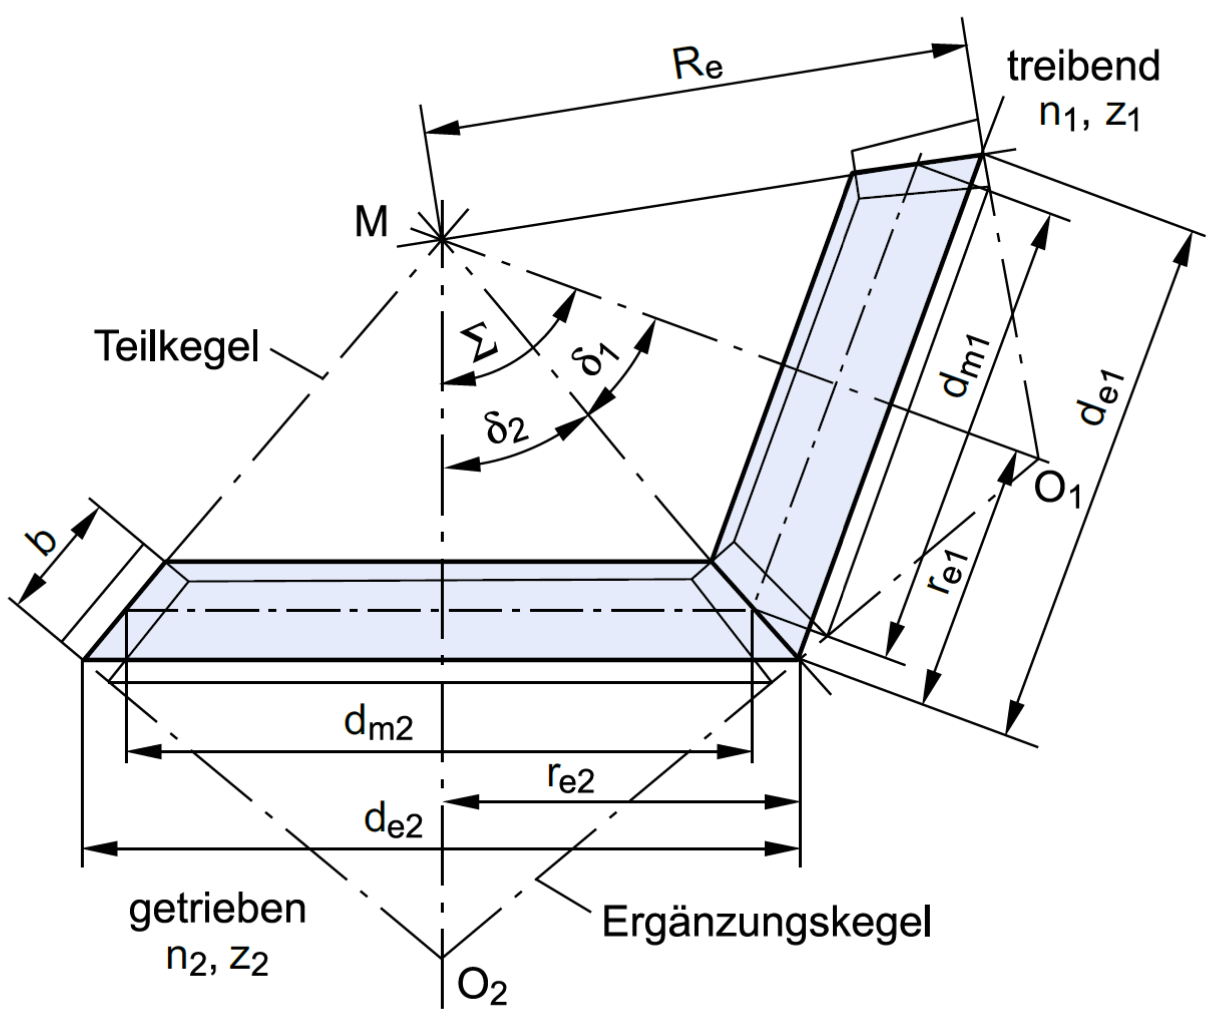
\includegraphics[width = 1.0\linewidth]{src/images/MAEIP_Kegelrad}}
    \end{center}
\end{minipage}
\vspace{-0.5mm}
\begin{footnotesize}
    \begin{empheq}[box=\fbox]{align*}
    &\text{Für $\Sigma \leq 90^\circ$:} \qquad \qquad \qquad \qquad \text{Für $\Sigma > 90^\circ$:}
    \\&tan(\delta_1) = \frac{sin(\Sigma)}{i + cos(\Sigma)} \; \; \; \; \qquad tan(\delta_1) = \frac{sin(180^\circ - \Sigma)}{i - cos(180^\circ - \Sigma)}
    \end{empheq}
    \begin{empheq}[box=\fbox]{align*}
        \Sigma = \delta_1 + \delta_2
    \end{empheq}
    \\\textbf{Kegelrad-Differential:}
    \mathbox{
        M_{an} = 2 \cdot M_{ab}
    }
\end{footnotesize} 
\vspace{0.1mm}

\subsubsection{Kräfte - Kegelrad \hfill ME}
\begin{minipage}{0.4\linewidth}
    \begin{footnotesize}
        \begin{center}
            \begin{empheq}[box=\fbox]{align*}
                F_{t1} = F_{t2} = \frac{2M_1}{d_{m1}}
            \end{empheq}
        \end{center}
    \end{footnotesize}
\end{minipage}
\begin{minipage}{0.58\linewidth}
    \begin{footnotesize}
        \begin{center}
            \mathbox{
                F_{r1} = F_{t1} \cdot tan(\alpha) \cdot cos(\delta_1)
            }
            \vspace{-2mm}
            \mathbox{
                F_{r2} = F_{t1} \cdot tan(\alpha) \cdot cos(\delta_2)
            }
            \vspace{-2mm}
            \mathbox{
                F_{a1} = F_{t1} \cdot tan(\alpha) \cdot sin(\delta_1)
            }
            \vspace{-2mm}
            \mathbox{
                F_{a2} = F_{t2} \cdot tan(\alpha) \cdot sin(\delta_2)
            }
        \end{center}
    \end{footnotesize}
\end{minipage}
    \subsection{Zykloid vs. Evolvent \hfill ME}
    \begin{scriptsize}
    \begin{itemize}
        \item \textbf{Zykloid:}
        \\\underline{Pro:} Konkave auf konvexe Fläche \\$\to$ geringe Flächenpressung $\to$ kleine ZR hochbelastbar
        \\\underline{Contra:} Keine gerade Eingriffslinie $\to$ Drehzahlschwankung bei Abweichung im \\Achsabstand $\to$ für jedes $z$ andere Fräser $\to$ hohe Fertigungskosten
        \item \textbf{Evolvent:}
        \\\underline{Pro:} Gerade Eingriffslinie $\to$ niedrige Fertigungskosten \\$\to$ undempfindlich ggü. Achsabstandänderung
        \\\underline{Contra:} Konvexe auf konvexe Fläche \\$\to$ hohe Flächenpressung $\to$ kleine ZR weniger belastbar
    \end{itemize}
\end{scriptsize}
    \subsection{Planetenradgetriebe \hfill ME}
\begin{itemize}
    \scriptsize{\item Generiert hohe Übersetzungen auf sehr kleinem Raum}
\end{itemize}
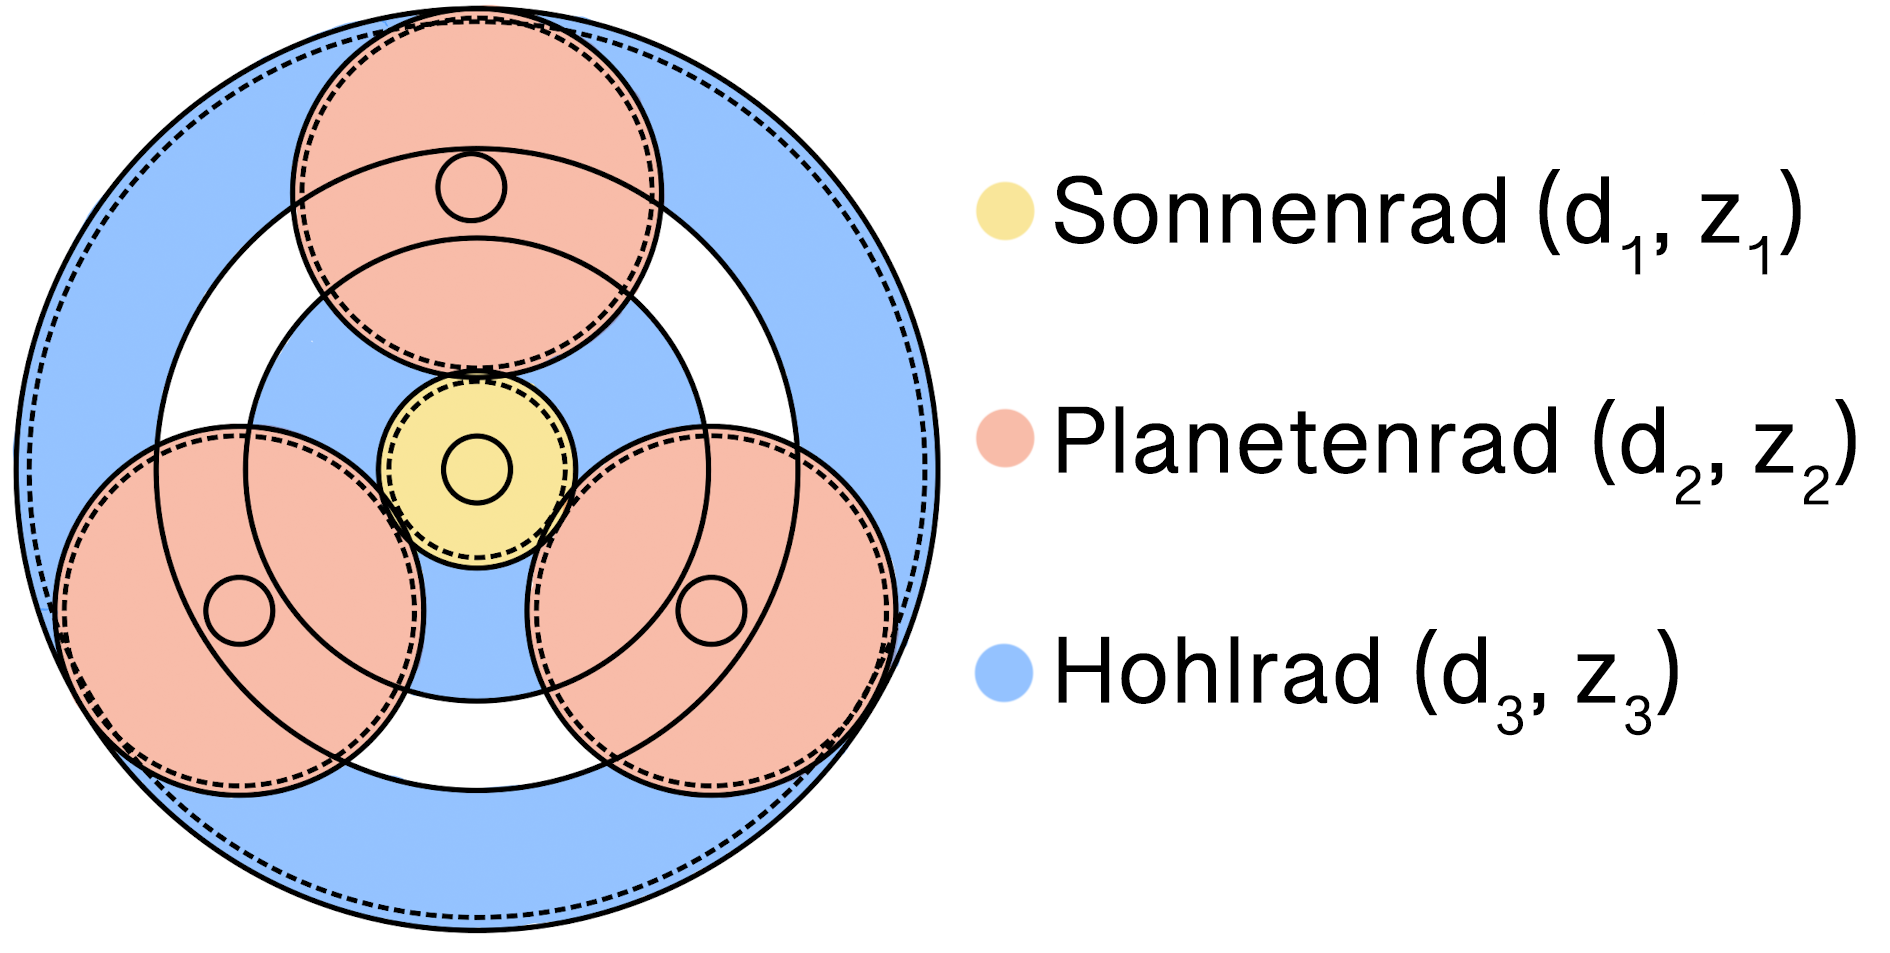
\includegraphics[width = 0.6\linewidth]{src/images/MAEIP_Planetenrad}
    \begin{footnotesize}
        \begin{center}
            \scriptsize{Innenverzahntes Rad besitzt per Definition negative Vorzeichen!}
            \begin{empheq}[box=\fbox]{align*}
                d_3 = 2\cdot d_2  + d_1 \quad &\mid \quad -z_3 = 2\cdot z_2 + z_1 \\
                \mathbb{Z} = \frac{|z_1| + |z_3|}{p} \quad &\mid \quad n_1 = (1-i_0)n_s +i_0n_3 \\
                i_0 = \frac{z_2}{z_1} \cdot \frac{z_3}{z_2} = \frac{n_1}{n_3} &= \frac{M_3}{M_1} = \frac{z_3}{z_1} = \frac{-d_3}{d_1}
            \end{empheq}
        \end{center}
    \end{footnotesize}
    \begin{scriptsize}
            $p = \text{Anzahl Planetenräder}; \; n_s = \text{Stegraddrehzahl}; \;i_0 = \text{Standübersetzung}$
    \end{scriptsize}
\par \vspace{1mm}\begin{center}
    \begin{footnotesize}
    \begin{tabular}{|c|c|c|c|}
        \hline
        An & Ab & Fest & $i(i_0 < 0)$\\
        \hline
        Sonne & Hohl & Steg & $i_0$\\
        \hline
        Hohl & Sonne & Steg & $1/i_0$\\
        \hline
        Sonne & Steg & Hohl & $1-i_0$\\
        \hline
        Steg & Sonne & Hohl & $1 / (1-i_0)$\\
        \hline
        Hohl & Steg & Sonne & $i_0 - (1/i_0)$\\
        \hline
        Steg & Hohl & Sonne & $i_0 / (i_0-1)$\\
        \hline 
     \end{tabular}
    \end{footnotesize}
\end{center}
    \subsection{Harmonic Drive \hfill ME}
\begin{center}
    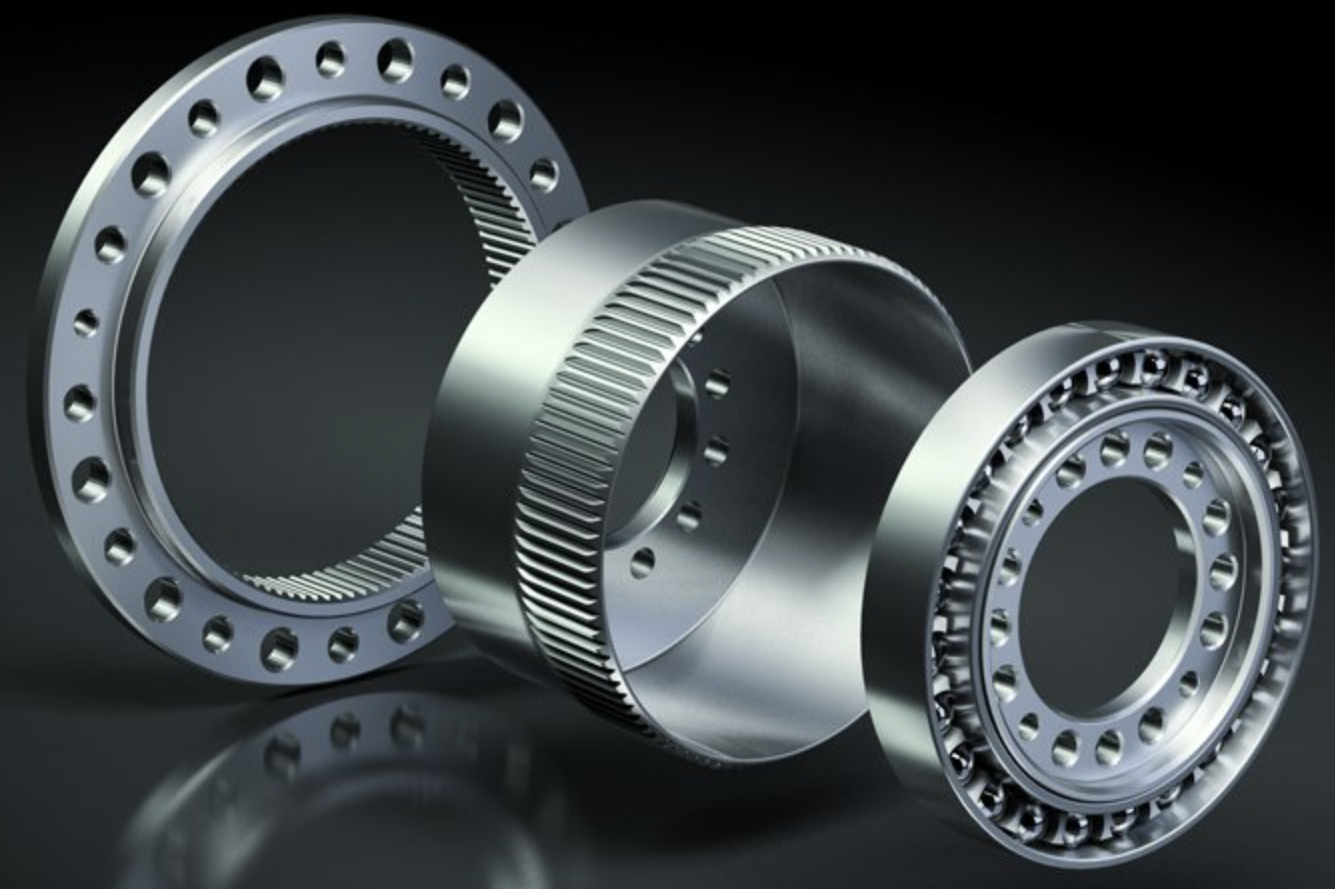
\includegraphics[width = 0.4\linewidth]{src/images/MAEIP_HarmonicDrive}
\end{center}
\begin{footnotesize}
    v.l.n.r.: Circular Spine (fest) $[z_3]$/ Flexspline (Abtrieb)$[n_2, z_2]$ / \\Wave Generator (Antrieb) $[n_1]$
    \begin{empheq}[box=\fbox]{align*}
        i &= \frac{n_1}{n_2} = -\frac{z_2}{2}
        \\z_3 &= -(z_2 + 2)
        \end{empheq}
\end{footnotesize}

\section{Schlussarten \hfill ME}
    \subsection{Stoffschluss \hfill ME}
\begin{itemize}
    \begin{scriptsize}
        \item Kraftübertragung durch \textbf{Molekularkräfte}
        \item \textbf{Adhäsion:} Haftkräfte an Kontaktfläche \underline{verschiedener} Werkstoffe
        \item \textbf{Kohäsion:} Haftkräfte an Kontakfläche \underline{eines} Werkstoffes
        \item \textbf{Nachteil:} nicht lösbare Verbindung $\to$ kann nur durch Zerstörung gelöst werden
        \item \textbf{Beispiele:} Kleben / Löten / Schweissen
    \end{scriptsize}
    \begin{footnotesize}
        \mathbox{
        F \leq F_{\text{scher}} = \tau_{\text{szul}} \cdot A \quad \mid \quad \tau = \text{Schubspn.} = \frac{F}{A}
    }
    \centering $A$ = Scherfläche (rot)
    \begin{center}
        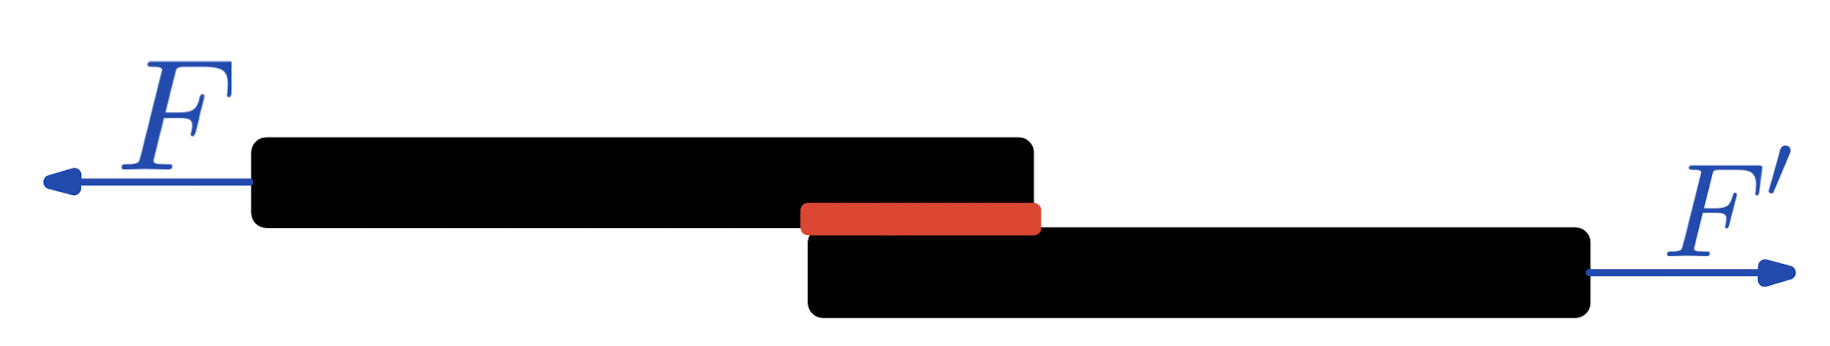
\includegraphics[width = 0.5\linewidth]{src/images/MAEIP_Stoffschluss}
    \end{center}
    \end{footnotesize}
\end{itemize}
    \subsection{Reibschluss \hfill ME}
\begin{scriptsize}
    \begin{itemize}
        \item Kraftübertragung durch \textbf{Normalkraft}
        \item \textbf{Beispiele:} Federn / Schrauben / Keile / Rad od. Fahrbahn
    \end{itemize}
\end{scriptsize}
\begin{footnotesize}
    \mathbox{
        F \leq F_R = \mu \cdot F_N
    }
    \begin{center}
        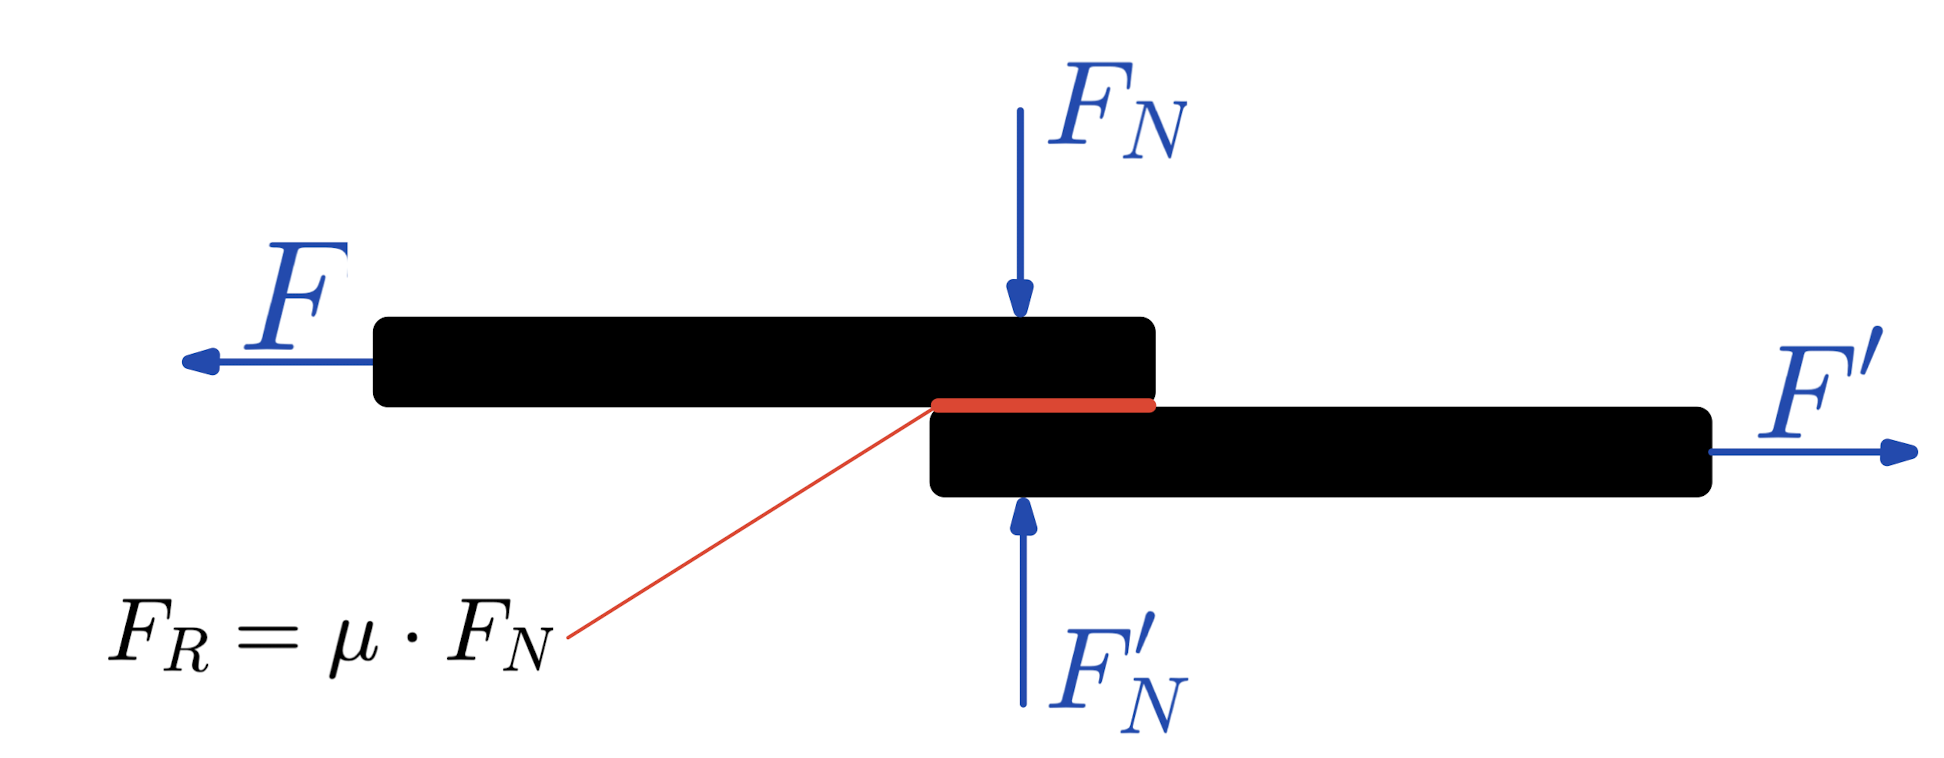
\includegraphics[width =0.6\linewidth]{src/images/MAEIP_Reibschluss}
    \end{center}
\end{footnotesize}
\subsubsection{Reibkraft \hfill ME}
    \vspace{-0.5em}
    \begin{minipage}{0.58\linewidth}
        \begin{footnotesize}
            \begin{center}
                \begin{empheq}[box=\fbox]{align*}
                    F_{\text{res}} &= \sqrt{F_t^2 + F_a^2}
                    \\ F_t &= \frac{2\cdot M_2}{d}
                    \\ F_r &= F_{\text{res}} \cdot S_R = F_N \cdot \mu_H
                    \\ &= p \cdot A \cdot \mu_H = p(\pi d l) \cdot \mu_H
                    \\ A &= \pi \cdot l_{tr} \cdot d
                    \end{empheq}
            \end{center}
        \end{footnotesize}
    \end{minipage}
    \begin{minipage}{0.38\linewidth}
        \begin{scriptsize}
            \begin{center}
                \begin{align*}
                    S_R &= \text{Sicherheitsfaktor} \\ & \text{gegen Rutschen}
                    \\F_a &= \text{axiale Kräfte}
                    \\ A &= \text{Fläche}
                    \\ \mu_H &= \text{Haftreibung}
                    \\ F_t &= \text{Tangential/Umfangskraft}
                    \\(\text{greift} &\text{ direkt an Welle an})
                \end{align*}
            \end{center}
        \end{scriptsize}
    \end{minipage}
\vspace{0.1em}

\subsubsection{Fugenpressung \hfill ME}
\vspace{-0.5em}
\begin{footnotesize}
    \begin{minipage}{0.6\linewidth}
        \begin{center}
            \begin{empheq}[box=\fbox]{align*}
                p_{\text{min}} &= \frac{F_{\text{res}}}{\mu_H \cdot \pi \cdot d \cdot l_{\text{tr}}}
                = \frac{F_{\text{res}}}{\mu_H \cdot A}
                \\p_{\text{max}} &\Rightarrow \sigma_V < \sigma_{\text{zul}}
            \end{empheq}
        \end{center}
    \end{minipage}
    \begin{minipage}{0.38\linewidth}
        \begin{center}
            \begin{align*}
                \scriptstyle p = \text{Fugendruck}\\
            \end{align*}
        \end{center}
    \end{minipage}
\end{footnotesize}
\vspace{0.1em}

\subsubsection{Übermass U\hfill ME}
\vspace{-0.5em}
\begin{footnotesize}
   \begin{minipage}{0.6\linewidth}
       \begin{center}
           \begin{empheq}[box=\fbox]{align*}
              G &= 0.4 \cdot (R_{Wa} + R_{Ni}) 
              \\U &= U_{\text{theo}} + G
              \\U_{\text{theo}} &= d_{Wa} - d_{Ni}
              \\U_{\text{max}} &= d_{Wa, \text{max}} - d_{Ni, \text{min}}
              \\U_{\text{min}} &= d_{Wa, \text{min}} - d_{Ni, \text{max}}
           \end{empheq}
       \end{center}
   \end{minipage}
   \begin{minipage}{0.38\linewidth}
       \begin{center}
           \begin{scriptsize}
           \begin{align*}
               G &= \text{Glättung}
               \\U &= \text{Übermass}
           \end{align*}
        \end{scriptsize}
       \end{center}
   \end{minipage}
\end{footnotesize}
\vspace{0.1em}

\subsubsection{Sicherheit gegen Rutschen \hfill ME}
\vspace{-0.5em}
\begin{footnotesize}
        \begin{center}
            \begin{empheq}[box=\fbox]{align*}
                S_R &= \frac{R}{B} = \frac{M_{t, \text{max}}}{M_t}
                \\M_{t, \text{max}} &= \frac{1}{2} \cdot d \cdot F_{t, \text{max}} = \frac{1}{2} \cdot d \cdot \mu \cdot F_{\text{Fuge}}
                \\ &= \frac{1}{2} \cdot d \cdot \mu \cdot p_{\text{Passung}} \cdot A = \frac{1}{2} \cdot d \cdot \mu \cdot p_{\text{Passung}} \cdot \pi \cdot l \cdot d
            \end{empheq}
        \end{center}
\end{footnotesize}
\vspace{0.1em}

\subsubsection{Kegelpressverband (KPV) \hfill ME}
\begin{footnotesize}
    \begin{minipage}{0.3\linewidth}
        \begin{center}
            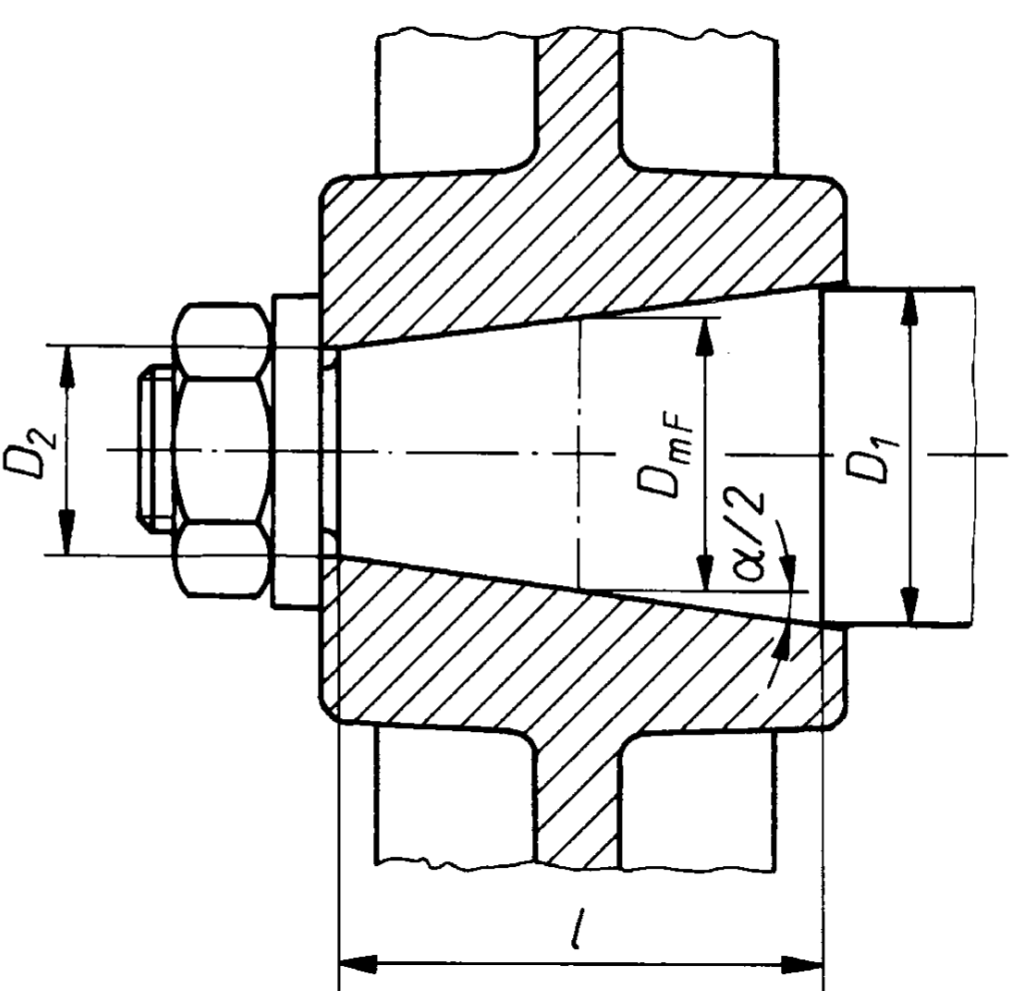
\includegraphics[width = 1.0\linewidth]{src/images/MAEIP_Kegelpressverband}
        \end{center}
    \end{minipage}
    \begin{minipage}{0.68\linewidth}
        \begin{center}
            \begin{empheq}[box=\fbox]{align*}
                p_{erf} &= \frac{2 \cdot \cos{\frac{\alpha}{2}} \cdot M_{max}}{\mu \cdot \pi \cdot D_{mF}^2 \cdot l}
                \\D_{mF} &= \frac{D_1 + D_2}{2} \; \mid \; \Delta l = \frac{U}{2 \cdot tan(\alpha)}
                \\U &= U_{\text{theo}} + 0.8(R_{ZW} + R_{ZN})
                \\D_2 &= D_1 - 2 l \tan{\frac{\alpha}{2}} = D_1 - l K
                \\K &= \text{Kegelverhältnis}
            \end{empheq}
        \end{center}
    \end{minipage}
\end{footnotesize}
\vspace{0.1em}

\subsubsection{Zylindrischer Pressverband (ZPV) \hfill ME}
\begin{footnotesize}
    \begin{minipage}{0.3\linewidth}
        \begin{center}
            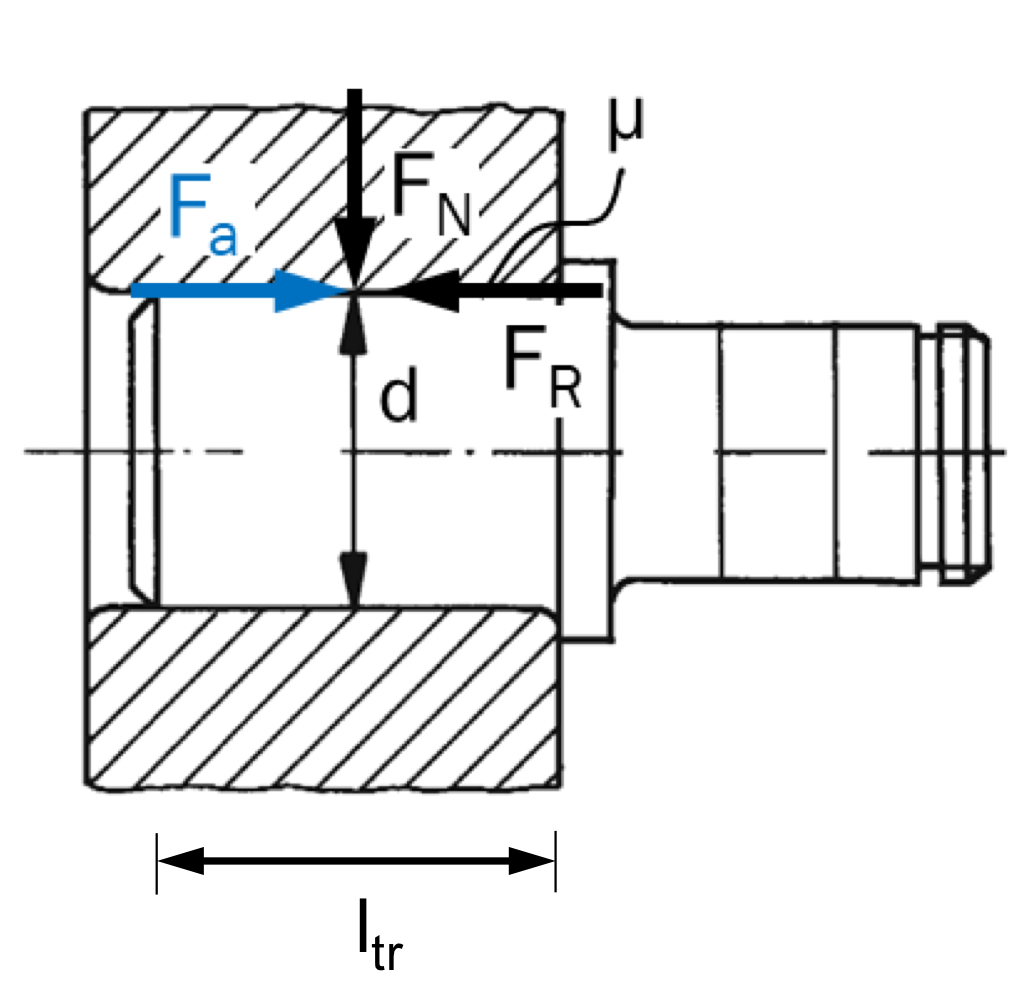
\includegraphics[width = 1.0\linewidth]{src/images/MAEIP_Zylindrischer_Pressverband}
        \end{center}
    \end{minipage}
    \begin{minipage}{0.58\linewidth}
        \begin{center}
            \mathbox{
                p_{erf} = \frac{F_{res,max}}{\mu \cdot \pi \cdot d \cdot l_{tr}}
            }
            \scriptsize{$F_{res,max} = \sqrt{F_{t,max}^2 + F_{a,max}^2}$} 
        \end{center}
    \end{minipage}
\end{footnotesize}
    \subsection{Formschluss \hfill ME}
\begin{footnotesize}
    \begin{scriptsize}
        \begin{itemize}
        \item Kraftübertragung durch \textbf{Scherwiderstand}
        \item Erhöhte Kerbwirkung und Flächenpressung
        \item \textbf{Beispiele:} Stifte / Passfedern / Schrauben / Verzahnungen
        \end{itemize}
    \end{scriptsize}
    \begin{empheq}[box=\fbox]{align*}
        F \leq F_{\text{scher}} = \tau_{\text{szul}} \cdot S \quad &\mid \quad S = c \cdot A
        \\ c_{\text{eckig}} = 0.75 \quad \mid \quad c_{\text{rund}} &= 0.66 \quad \mid \quad c_{\text{hohl}} = 0.5
    \end{empheq}
    \begin{center}
        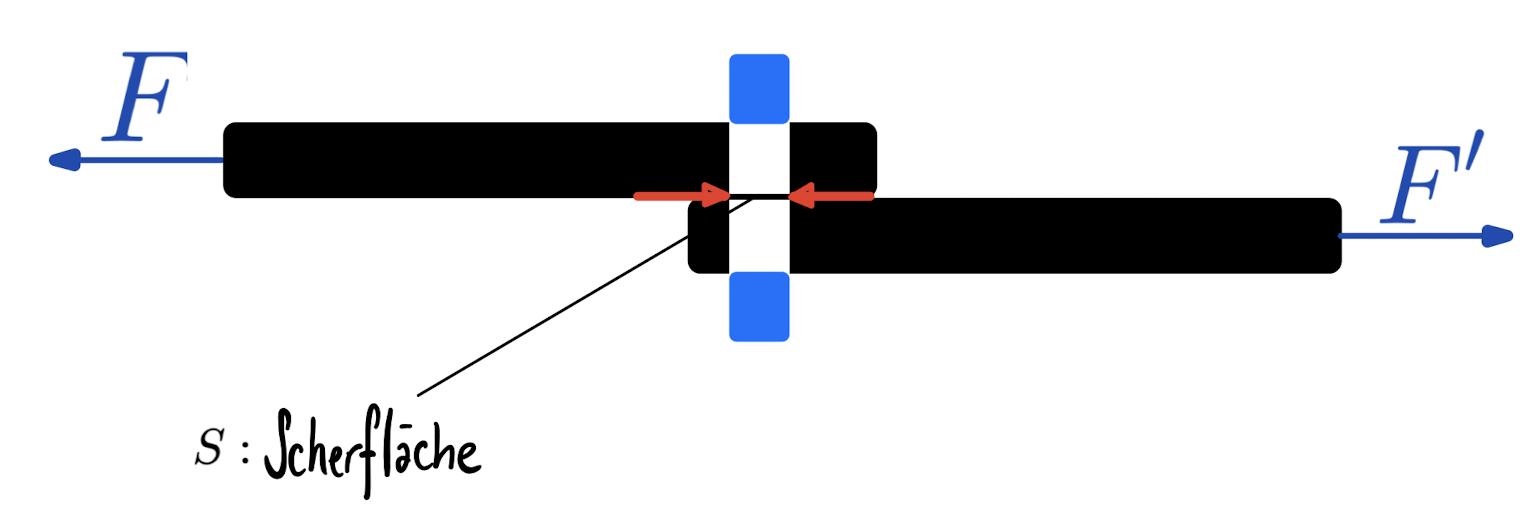
\includegraphics[width = 0.5 \linewidth]{src/images/MAEIP_Formschluss}
    \end{center}
\end{footnotesize}

\subsubsection{Passfeder \hfill ME}
\begin{scriptsize}
   \begin{itemize}
       \item \textbf{Kritische Bauteile:} Nabe, Welle $\to$ Flächenpressung, Schubspannung
   \end{itemize}
\end{scriptsize}
   \begin{minipage}{0.48\linewidth}
    \begin{center}
        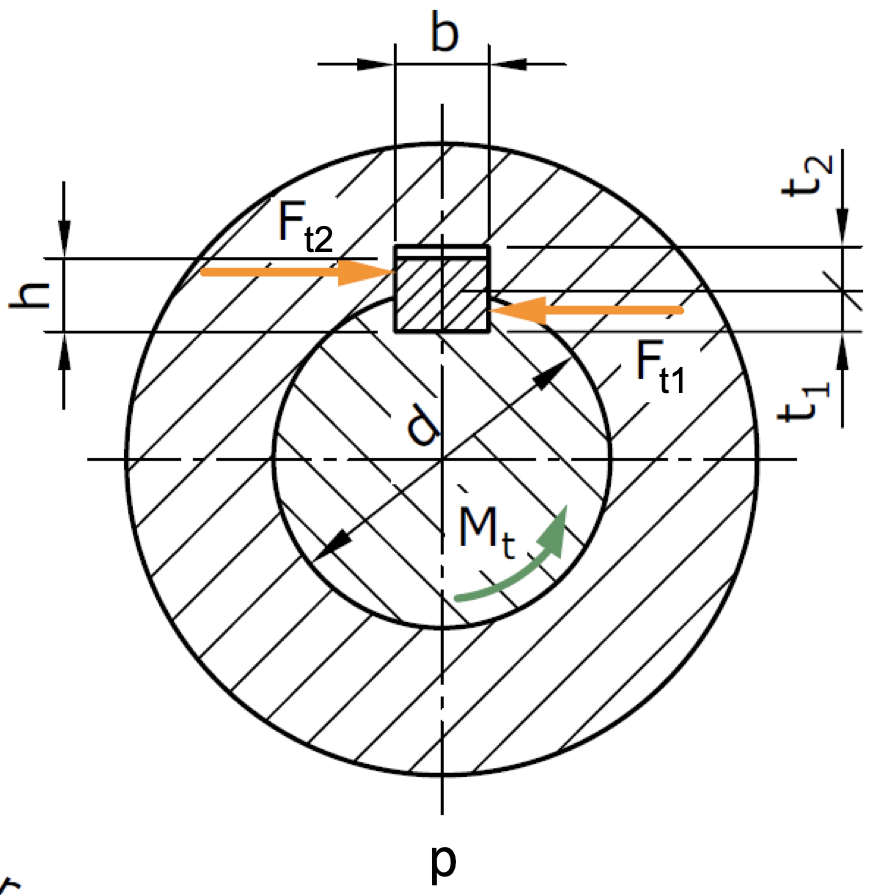
\includegraphics[width = 1.0\linewidth]{src/images/MAEIP_Passfeder}
    \end{center}
   \end{minipage}
   \begin{scriptsize}
    \begin{minipage}{0.5\linewidth}
        \begin{center}
           \begin{align*}
                p_w &= \text{Flächenpressung}
               \\p_m &= \text{Mittlere Pressung}
               \\f_s &= \text{Stützfaktor}
               \\f_h &= \text{Härteeinflussfaktor}
               \\n &= \text{Anzahl Passfedern}
               \\l_{tr}&= \text{tragende Länge}
               \\t_1 &= \text{Nuttiefe}
               \\\varphi &= \text{Traganteil} 
               \\ &= 1 \; \text{(für n=1)}
               \\ &= 0.75 \; \text{(für n=2)}
               \\c_b &= \text{Betriebsfaktor}
               \\h &= \text{Höhe}
               \\K_t &= \text{Techn. Grössenfaktor}
            \end{align*}
        \end{center}
   \end{minipage}
   \end{scriptsize}
   \begin{footnotesize}
       \mathbox{
        p_{\text{zul}} = f_s \cdot f_h \cdot \frac{R_e}{S_F} = f_s \cdot f_h \cdot \frac{K_t \cdot R_{e,N}}{S_F} = f_s \cdot \frac{R_{p0.2}}{S_F}
       }
   \end{footnotesize}
\begin{footnotesize}
\begin{empheq}[box=\fbox]{align*} 
    &M_{t, \text{max}} = \frac{p_{\text{zul}} \cdot d \cdot l_{tr}(h-t_1) \cdot n}{2} < c_b \cdot M_{\text{nenn}}
    \\ &p_w = \frac{F_U}{(h-t)\cdot l_{tr} \cdot n \cdot \varphi} = \frac{2\cdot M_t}{d\cdot(h-t) \cdot l_{tr} \cdot n \cdot \varphi} \leq p_{zul}
    \\ &p_m = \frac{2 \cdot M_t}{d \cdot (h - t) \cdot l_{tr}}
    \\ &\text{Form A \cornersize{5} \ovalbox{Passfeder}}: \; l_{\text{tragend}} = l -(2r) = l-b
    \\ &\text{Form B \fbox{Passfeder}}: \; l_{\text{tragend}} = l
\end{empheq}



\begin{itemize}
    \item \textbf{Wertetabelle für $c_b$:}
    \\ \hspace{-7mm}\begin{tabular}{ |c|c|c|c|c|}
        \hline
        $c_b$ & Ab &&&\\
        \hline
        An & gleichmässig & $\uparrow$ Stösse & $\uparrow \uparrow$ Stösse & $\uparrow \uparrow \uparrow$ Stösse\\
        \hline
        gleichmässig & 1.0 & 1.25 & 1.5 & 1.75\\
        \hline
        $\uparrow$ Stösse & 1.1 & 1.35 & 1.6 & 1.85\\
        \hline
        $\uparrow \uparrow$ Stösse & 1.25 & 1.5 & 1.75 & 2.0\\
        \hline
        $\uparrow \uparrow \uparrow$ Stösse & 1.5 & 1.75 & 2.0 & 2.25\\
        \hline

    \end{tabular}
    \item \textbf{Beschriftung:} DIN 6885 - $\colorbox{pink}{A} \quad \colorbox{Thistle}{14} \quad \text{x} \quad \colorbox{Apricot}{9} \quad \text{x} \quad \colorbox{Melon}{36}$
    \\ \hspace{25mm}\colorbox{pink}{Form} / \colorbox{Thistle}{Breite} / \colorbox{Apricot}{Höhe} / \colorbox{Melon}{Länge}
\end{itemize}
\end{footnotesize}

\cbreak

\subsubsection{Keilwelle \hfill ME}
    \begin{scriptsize}
        \begin{itemize}
            \item grose, wechselnde, stossartige Drehmomente
            \item Kerbwirkung: $\downarrow$ Biegung, $\uparrow$ Torsion $\Rightarrow$ Kosten hoch
        \end{itemize}
    \end{scriptsize}
    \begin{minipage}{0.36\linewidth}
        \begin{center}
            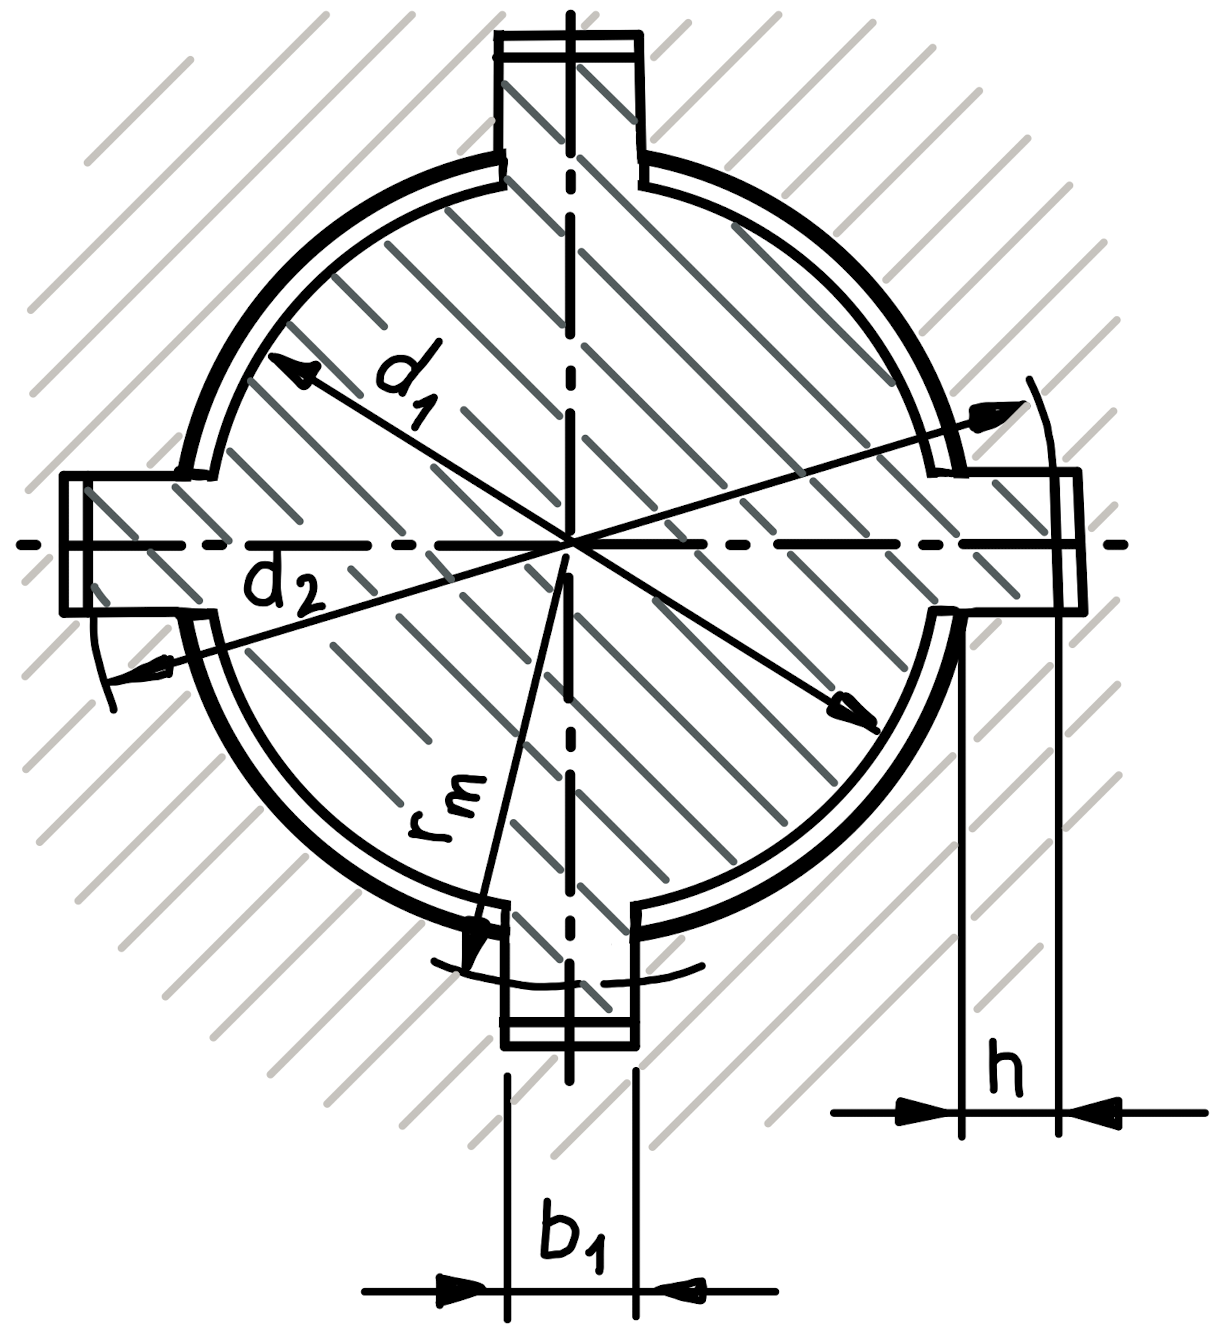
\includegraphics[width = 1.0\linewidth]{src/images/MAEIP_Keilwelle}
        \end{center}
    \end{minipage}
    \begin{minipage}{0.62\linewidth}
        \begin{center}
            \begin{scriptsize}
                \begin{align*}
                    n &= \text{Anzahl Keile}
                    \\l_{tr} = L_N &= \text{tragende Länge}
                    \\\varphi &= 0.9 \; (\text{Flankenzentrierung})
                    \\\varphi &= 0.75 \; (\text{Innenzentrierung})
                \end{align*}
            \end{scriptsize}
            \begin{footnotesize}
                \begin{empheq}[box=\fbox]{align*}
                    r_m &= \frac{d_1 + d_2}{4}
                    \\h &= 0.5 \cdot (d_{2,W} -d_{1,N})
                    \\h_{tr} &\approx 0.4 \cdot (d_{2} - d_{1})
                    \\M_{t, \text{max}} &= h_{tr} \cdot l_{tr} \cdot p_{\text{zul}} \cdot r_m \cdot \varphi \cdot n
                    \\p_m &= \frac{10 \cdot M}{(D+d) l_{tr} (D-d) n \cdot \varphi}
                \end{empheq}
            \end{footnotesize}
        \end{center}
    \end{minipage}

\section{Wellendimensionierung \hfill ME}
    \begin{footnotesize}
    \mathbox{
        \sigma_b = \frac{M_b}{W_b} \quad \mid \quad \tau_t = \frac{M_t}{W_t} \quad \mid \quad d_{\text{min}} > \sqrt[3]{\frac{16M_t}{\pi \cdot \tau_{t, \text{zul}}}}
    }
    
    % \begin{empheq}[box=\fbox]{align*}
    %      \quad \mid \quad \text{\scriptsize\underline{nur Torsion: } } d_{\text{min}} > \sqrt[3]{\frac{16 M_t}{\pi \cdot \tau_{\text{zul}}}}
    % \end{empheq}

    \begin{empheq}[box=\fbox]{align*}
        \underline{\text{Vollwelle:}} \; W_b = \frac{\pi \cdot d^3}{32} \quad &\mid \quad W_t = \frac{\pi \cdot d^3}{16}    
        \\\underline{\text{Hohlwelle:}} \; W_b = \frac{\pi \cdot (D^4-d^4)}{32 \cdot D} \quad &\mid \quad W_t = \frac{\pi \cdot (D^4-d^4)}{16\cdot D}
    \end{empheq}
    \scriptsize{$\sigma_b$ = Biegespannung; $M_b$ = Biegemoment $[F\cdot r]$; \\$W_b$ od. $W_{ax}$ = axiales Widerstandsmoment; $M_t$ = Torsionsmoment $[F\cdot r]$; \\$W_t$ od. $W_{p}$ = polares Widerstandsmoment}
\end{footnotesize}
    \subsection{Wechselfestigkeit \hfill ME}
\begin{footnotesize}
    \begin{empheq}[box=\fbox]{align*}
        \sigma_v &= \sqrt{\sigma_b^2 + 3\tau_t^2} \quad \mid \quad S_D = \frac{R}{B} = \frac{\sigma_{b,W}}{\sigma_v} = \frac{\tau_{t,W,N}}{\tau_{t, \text{zul}}}
       \\ \sigma_v &= \sqrt{(\alpha_b \cdot \sigma_b)^2 + 3\cdot (\alpha_t \cdot \tau_t)^2} \quad \mid \quad \tau_{t, \text{zul}} = \frac{\tau_{t,W,N}}{S_D}
       \\ S_D &= 3 \text{ (kurze Welle)};\quad S_D = 4 \text{ (lange Welle)}
    \end{empheq}
    \scriptsize{$\sigma_v$ = Vergleichsspannung; $\sigma_{b,W}$ = Biege-Wechselfestigkeit; \\$\tau_{t,W,N}$ = Torsions-Wechselfestigkeit; $S_D$ = Sicherheit gegen Bruch}
\end{footnotesize}
    \subsection{Kerben \hfill ME}
\begin{footnotesize}
    \begin{minipage}{0.58\linewidth}
        \begin{center}
            \mathbox{
                \alpha_k = \frac{\sigma_{\text{max}}}{\sigma_n} = \frac{\tau_{\text{max}}}{\tau_n}
            }
        \end{center}
    \end{minipage}
    \begin{minipage}{0.4\linewidth}
        \begin{scriptsize}
            \begin{center}
                $\alpha_k$ = Kerbformzahl
                \\$\beta$ = Kerbwirkungszahl 
                \\$\sigma_n$ = Nennspannung $(= \sigma_b)$
                \\(Zustand ohne Kerbe)
                \\$\tau_n$ = Nenntorsion $(= \tau_t)$
            \end{center}
        \end{scriptsize}
    \end{minipage}
    \begin{itemize}
        \item \scriptsize Bei \underline{Umfangsnuten} (Freistich) und \underline{Wellenabsätzen} immer \textbf{kleineren} Durchmesser nehmen für Nennspannung ($\sigma_n, \tau_n$).
        \item \scriptsize Bei \underline{Passfedernuten} und \underline{Keilwellen} immer \textbf{grösseren} Durchmesser nehmen für Nennspannung ($\sigma_n, \tau_n$)
    \end{itemize}
\end{footnotesize}
\cbreak

\section{Lager und Lagerung \hfill ME}
    \begin{center}
    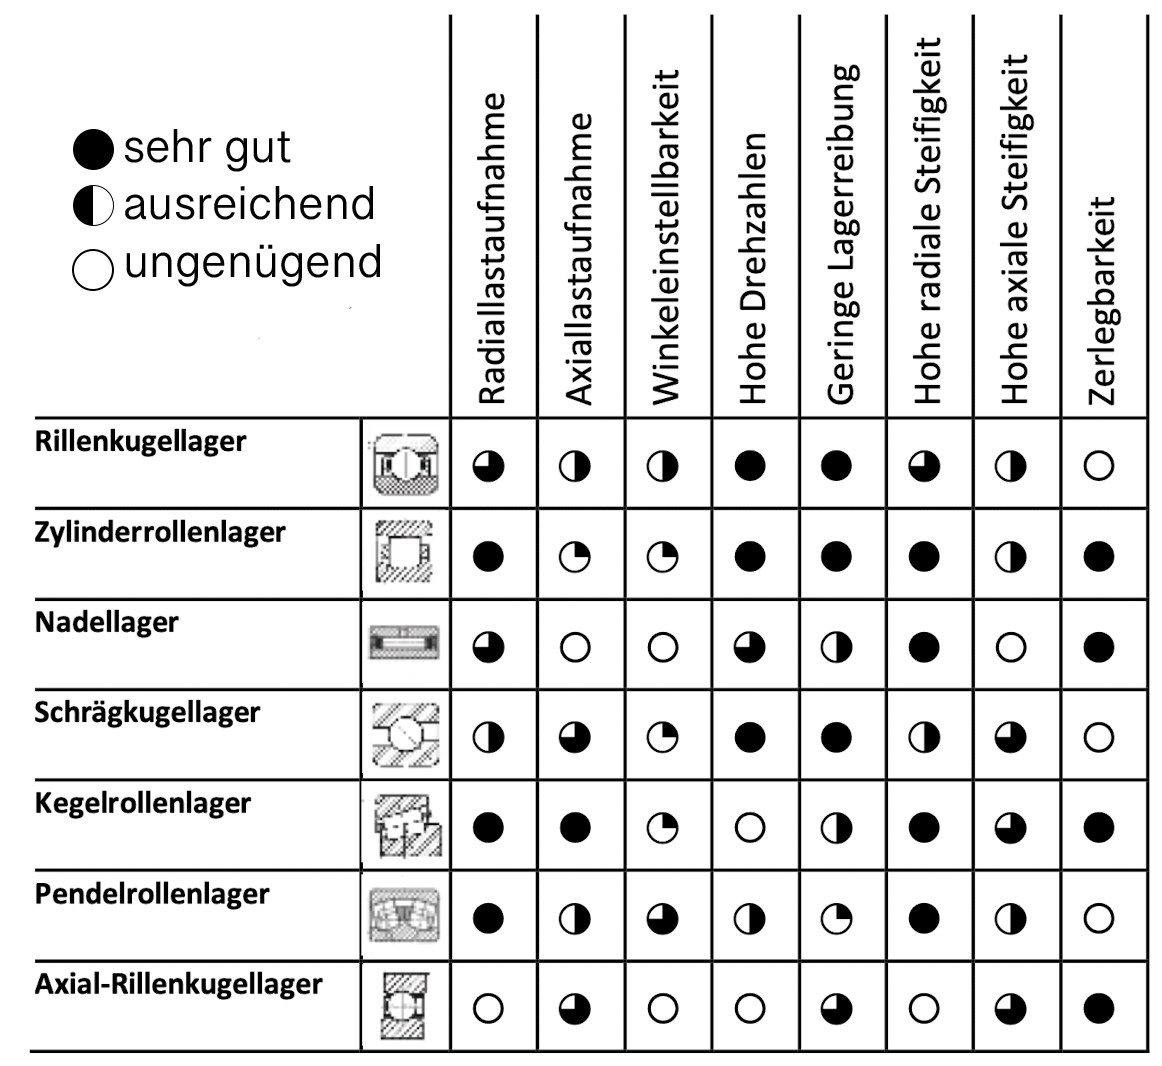
\includegraphics[width = 0.9\linewidth]{src/images/MAEIP_Lagerungen}
\end{center}
\begin{scriptsize}
    \begin{itemize}
        \item \textbf{Fest-Los:} \underline{Pro:} eindeutige Positionierung / Axialbelastung / Längen-\\ausgleich durch Loslager / statisch bestimmt
        \\ \underline{Contra:} zusätzliche Fertigungsschritte / hohe Kosten
        \item \textbf{Schwimmend:} \underline{Pro:} geringe Kosten / Längenausgleich
        \\ \underline{Contra:} keine wechselnde Axiallasten / schlechte Positionierungsgenauigkeit
        \item \textbf{Angestellt X:} \underline{Pro:} hohe Axialkräfte / hohe Positionierungsgenauigkeit / Kräfte zwischen Lager 
        \\ \underline{Contra:} hohe Kosten / kein Längenausgleich
        \item \textbf{Angestellt O:} \underline{Pro:} hohe Axialkraft / hohe Positionierungsgenauigkeit / Kräfte ausserhalb Lager
        \\ \underline{Contra:} hohe Kosten / kein Längenausgleich
        \\~\\
        \item \textbf{Passungswahl:} 
        \\ \textbf{Punktlast:} $\Rightarrow$ Spiel / \textbf{Umfangslast:} $\Rightarrow$ Übermass 
    \end{itemize} 
\end{scriptsize}
    \input{src/5_Lager/1_tragfähigkeit.tex}
    \subsection{Punkt und Umfangslast}
    \begin{center}
        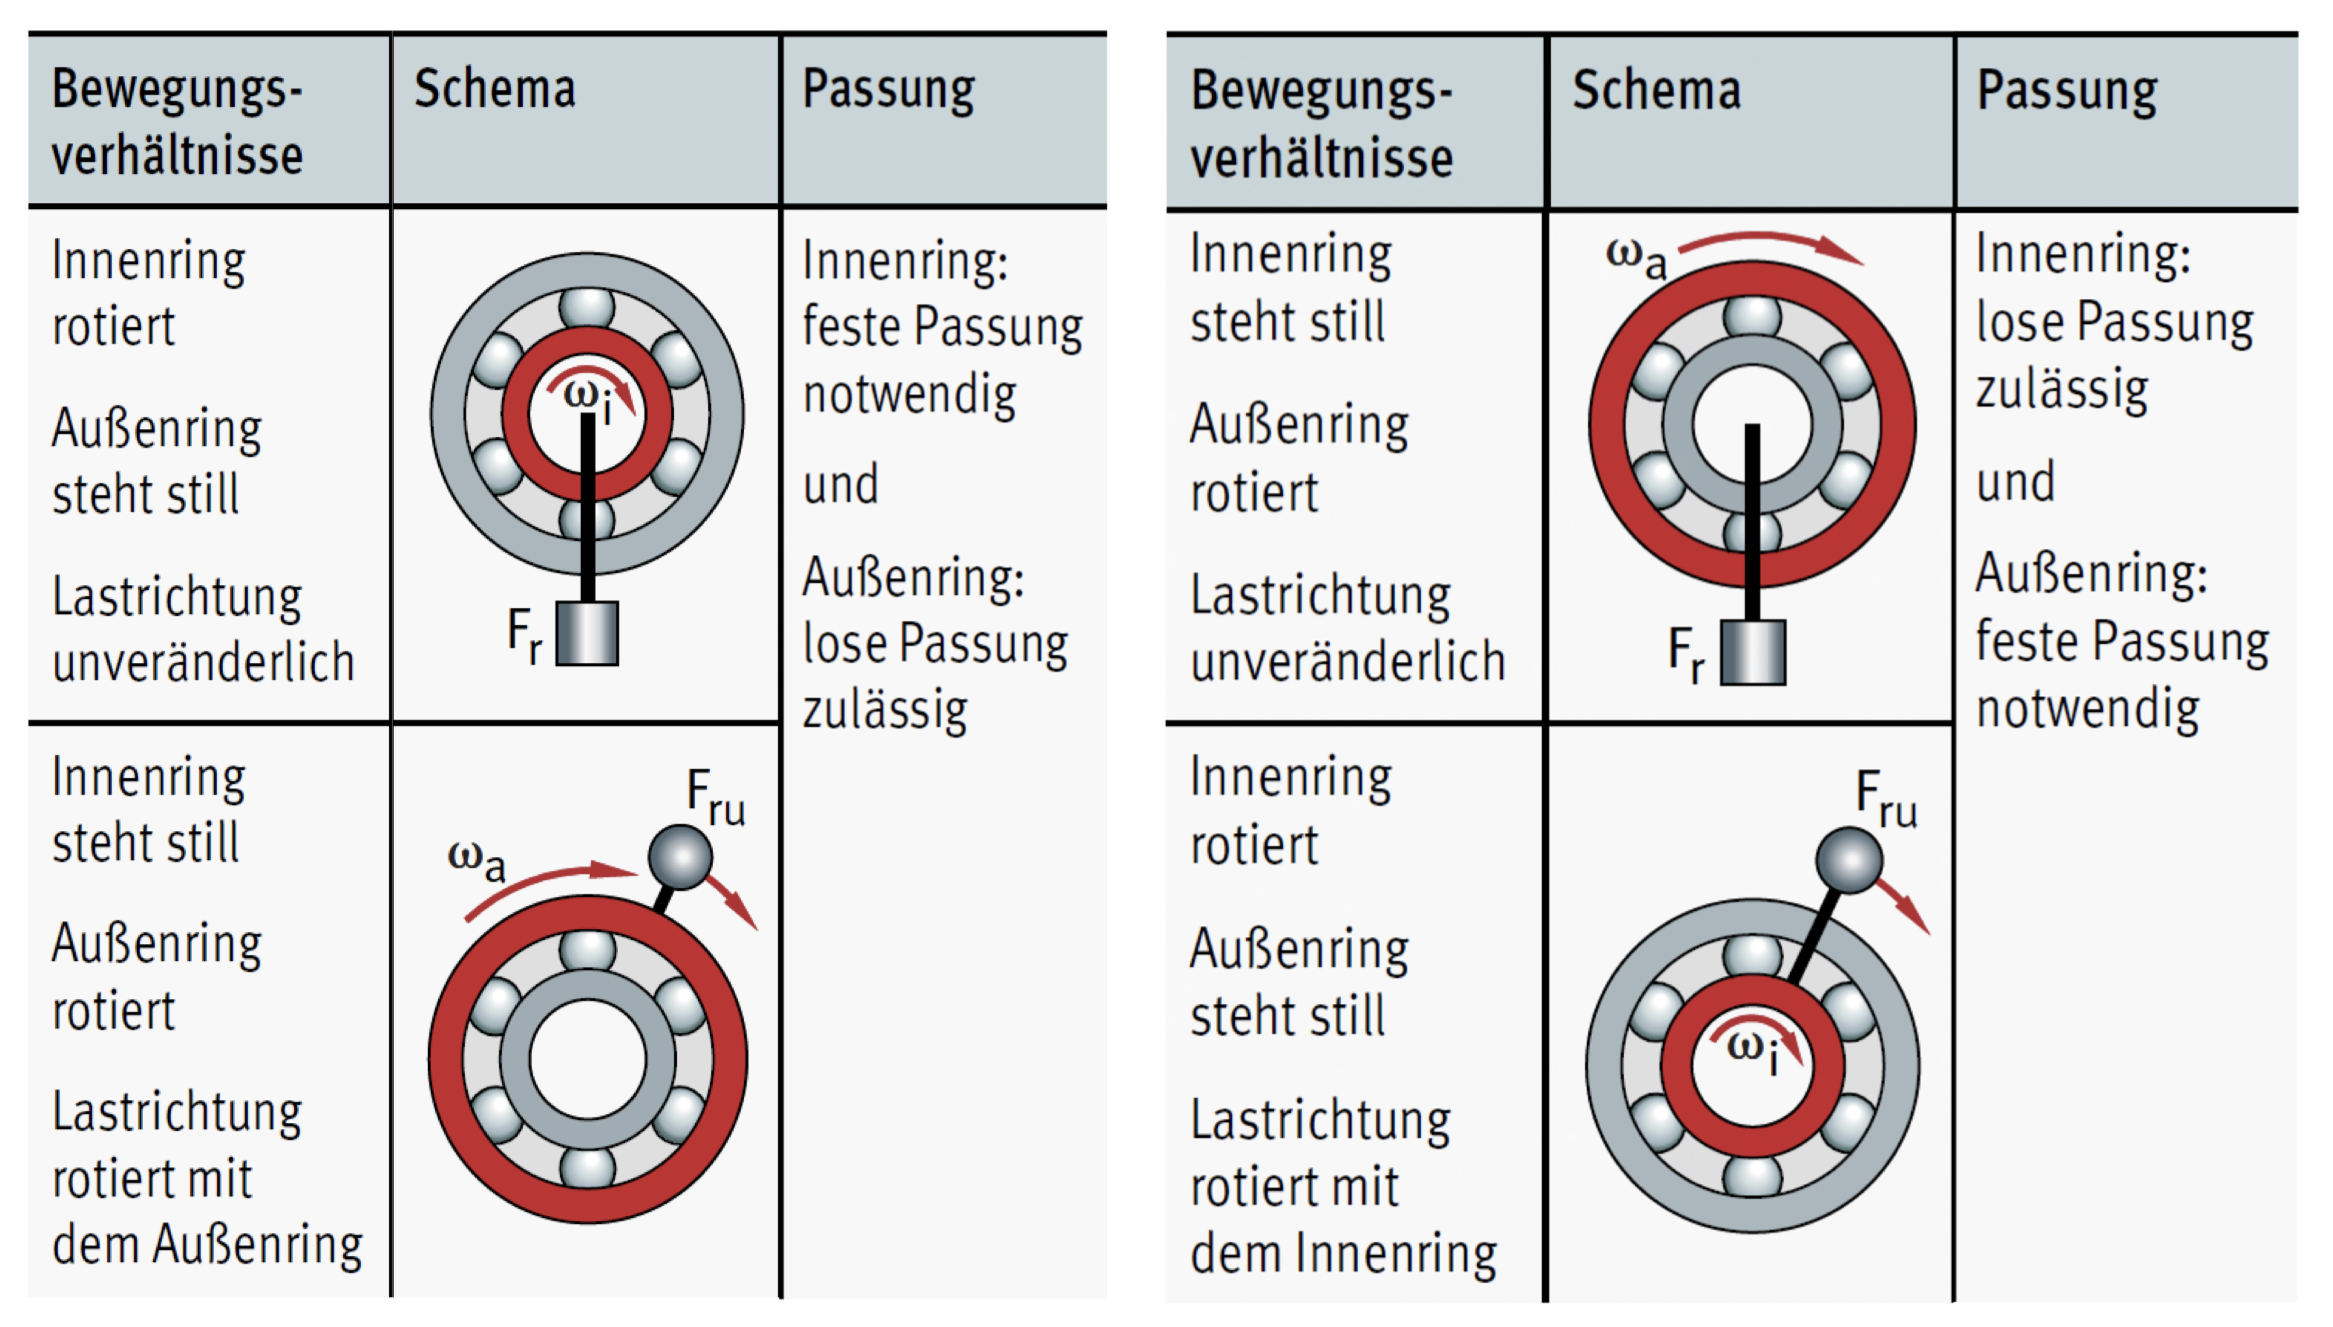
\includegraphics[width = 1.0\linewidth]{src/images/MAEIP_Lager_Punkt_Umfangslast.jpeg}
    \end{center}
    \cbreak

% \section{Schmierung \hfill ME}
%     \begin{scriptsize}
    \begin{itemize}
        \item \textbf{Funktionen:} tragfähiger Schmierfilm / Wärme ableiten / Verunreinigungen \\abdichten / Laufgeräusch dämpfen / Korrosion schützen
        \item \textbf{Öl:} \\\underline{Pro:} gute Verteilung / Ausspülen von Verschleisspartikeln / geringe Reibungsverluste \\bei Minimalmengenschmierung / Wärmeabfuhr möglich
        \\ \underline{Contra:} aufwändige Zuführung / Dichtung
        \item \textbf{Fett:} \\\underline{Pro:} geringer konstruktiver Aufwand / Dicht- und Depotwirkung / hohe Gebrauchs-\\dauer
        \\ \underline{Contra:} keine Wärmeabfuhr / kein Ausspülen von Verschleiss
        \item \textbf{Grenzschichtschmierung / Festkörperreibung:} Belastung wird von den \\Rauhigkeitsspitzen der Reibpartner getragen
        \item \textbf{Teilschmierung / Mischreibung:} Belastung wird vom Schmierfilm und \\durch Rauhigkeitsspitzen getragen
        \item \textbf{Vollschmierung / Flüssigkeitsreibung:} Der Schmierfilm nimmt die Belastung auf
    \end{itemize}
\end{scriptsize}
\section{Toleranzen und Passung}
    \subsection{Toleranzfeldbild}
    \begin{minipage}{0.99\linewidth}
        \begin{minipage}{0.49\linewidth}
            $\text{Toleranzfeld Welle}$
    
            \begin{raggedright}
                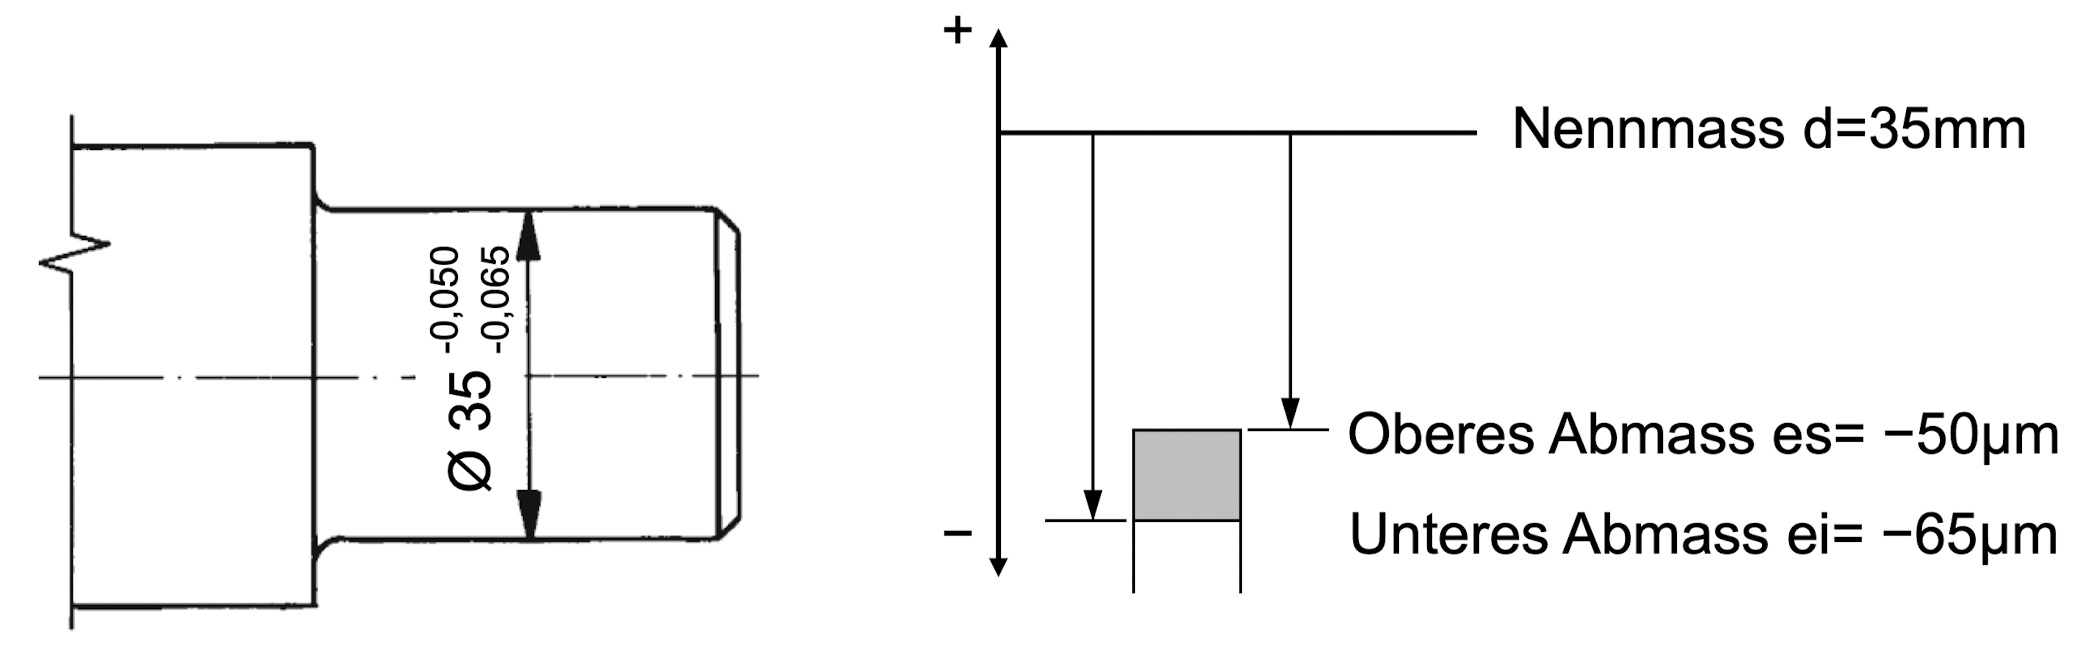
\includegraphics[width = 0.9\linewidth]{src/images/MAEIP_Toleranzfeld_Welle.png}
            \end{raggedright}
        \end{minipage}
        \begin{minipage}{0.49\linewidth}
            $\text{Toleranzfeld Bohrung}$
    
            \begin{raggedleft}
                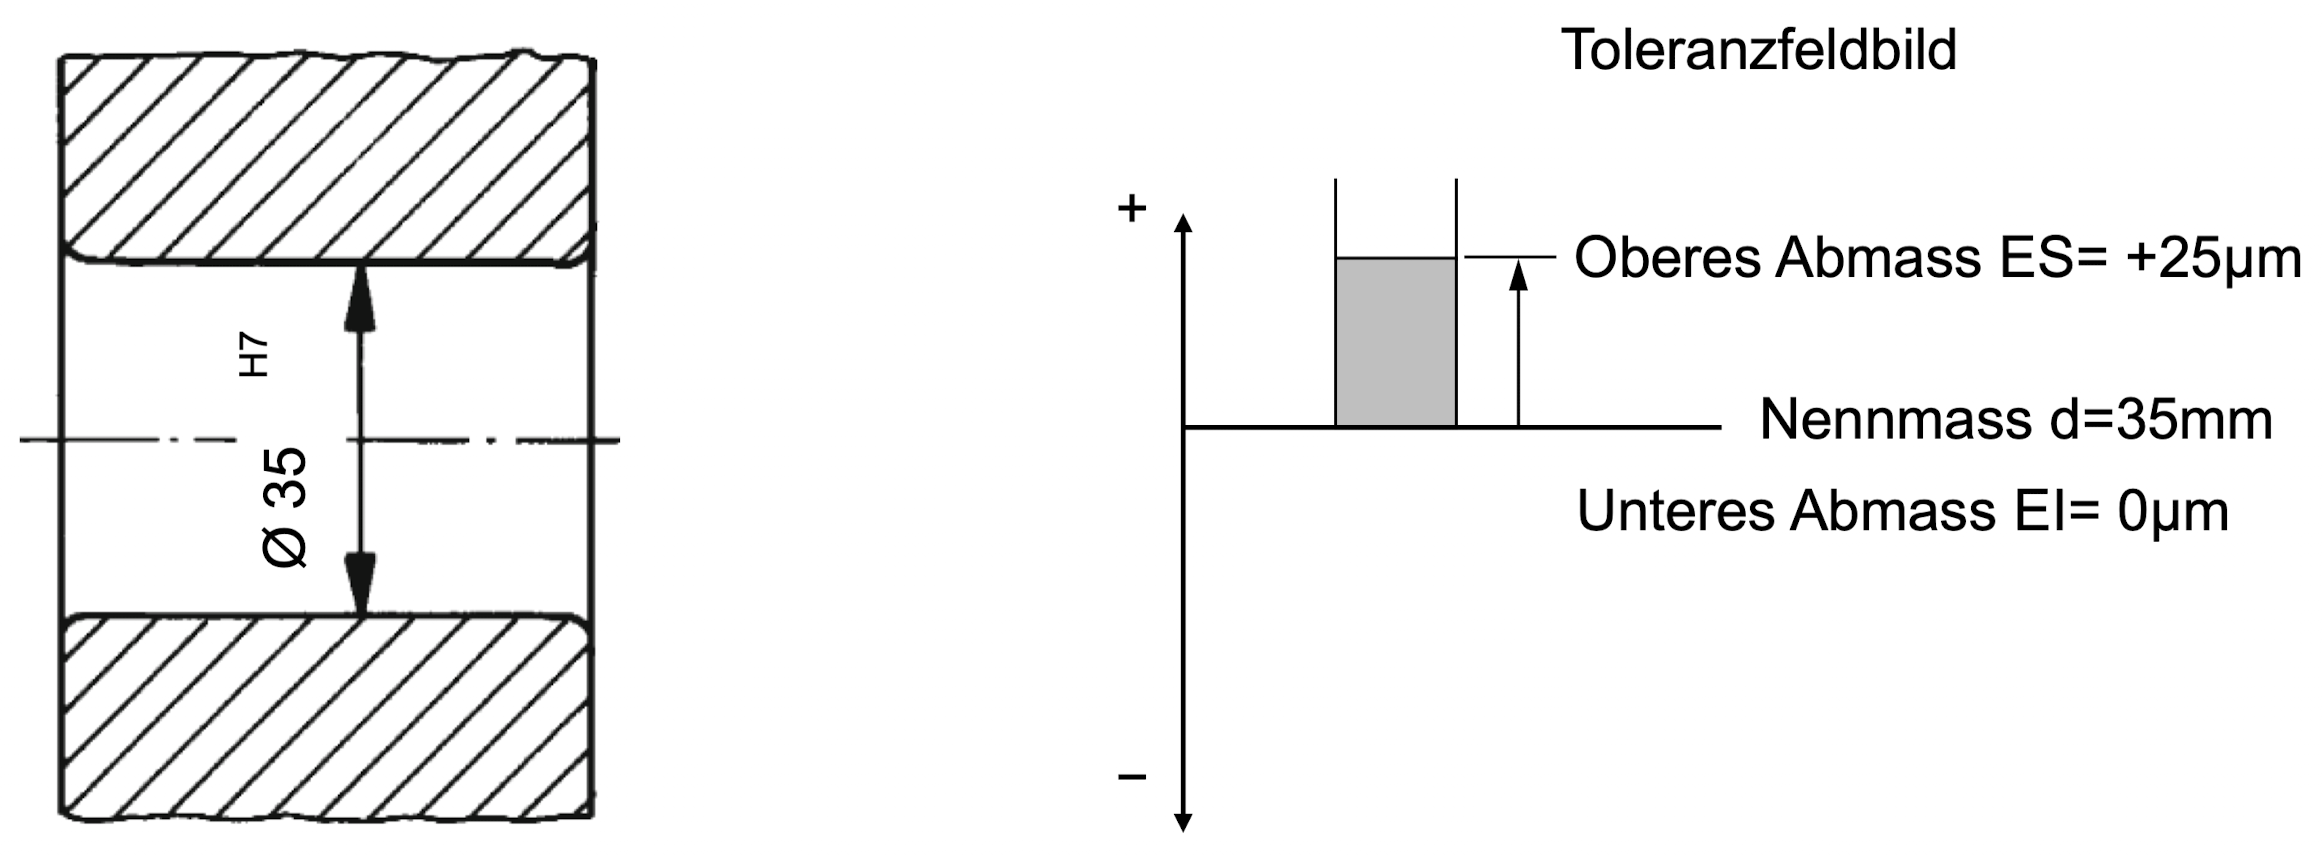
\includegraphics[width = 0.9\linewidth]{src/images/MAEIP_Toleranzfeld_Bohrung.png}
            \end{raggedleft}
        \end{minipage}
    \end{minipage}
    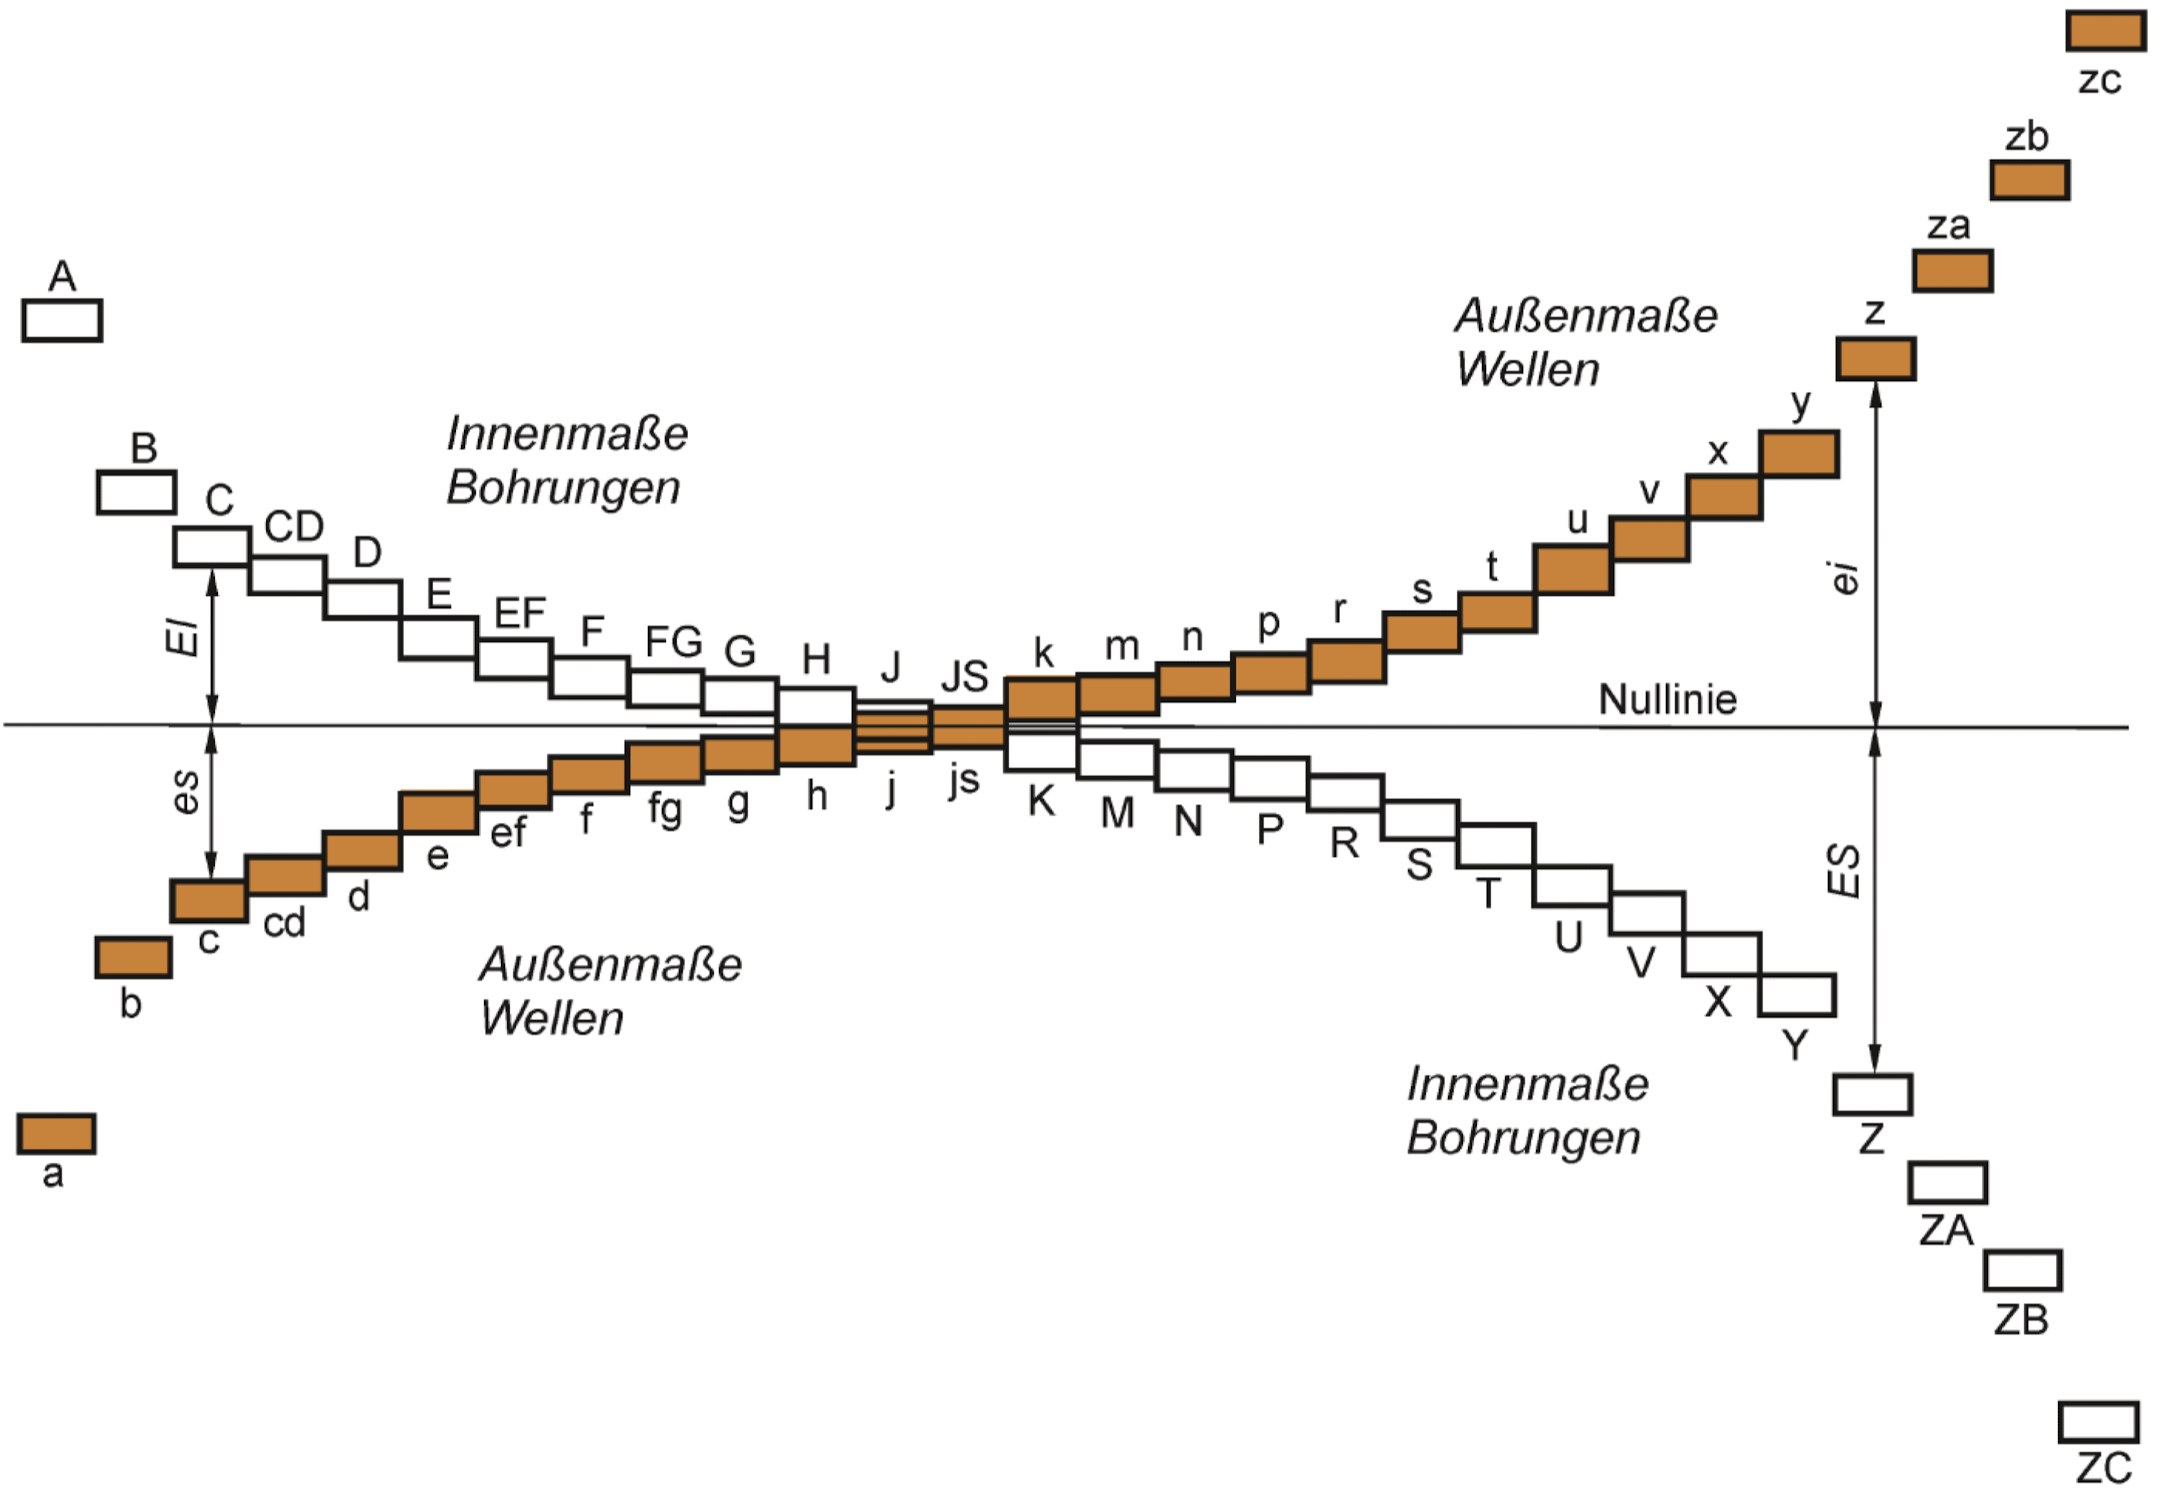
\includegraphics[width = 0.9\linewidth]{src/images/MAEIP_Toleranzfeld.png}
    \subsection{Passungen}
    \begin{minipage}{0.99\linewidth}
        \begin{minipage}{0.49\linewidth}
            \begin{center}
                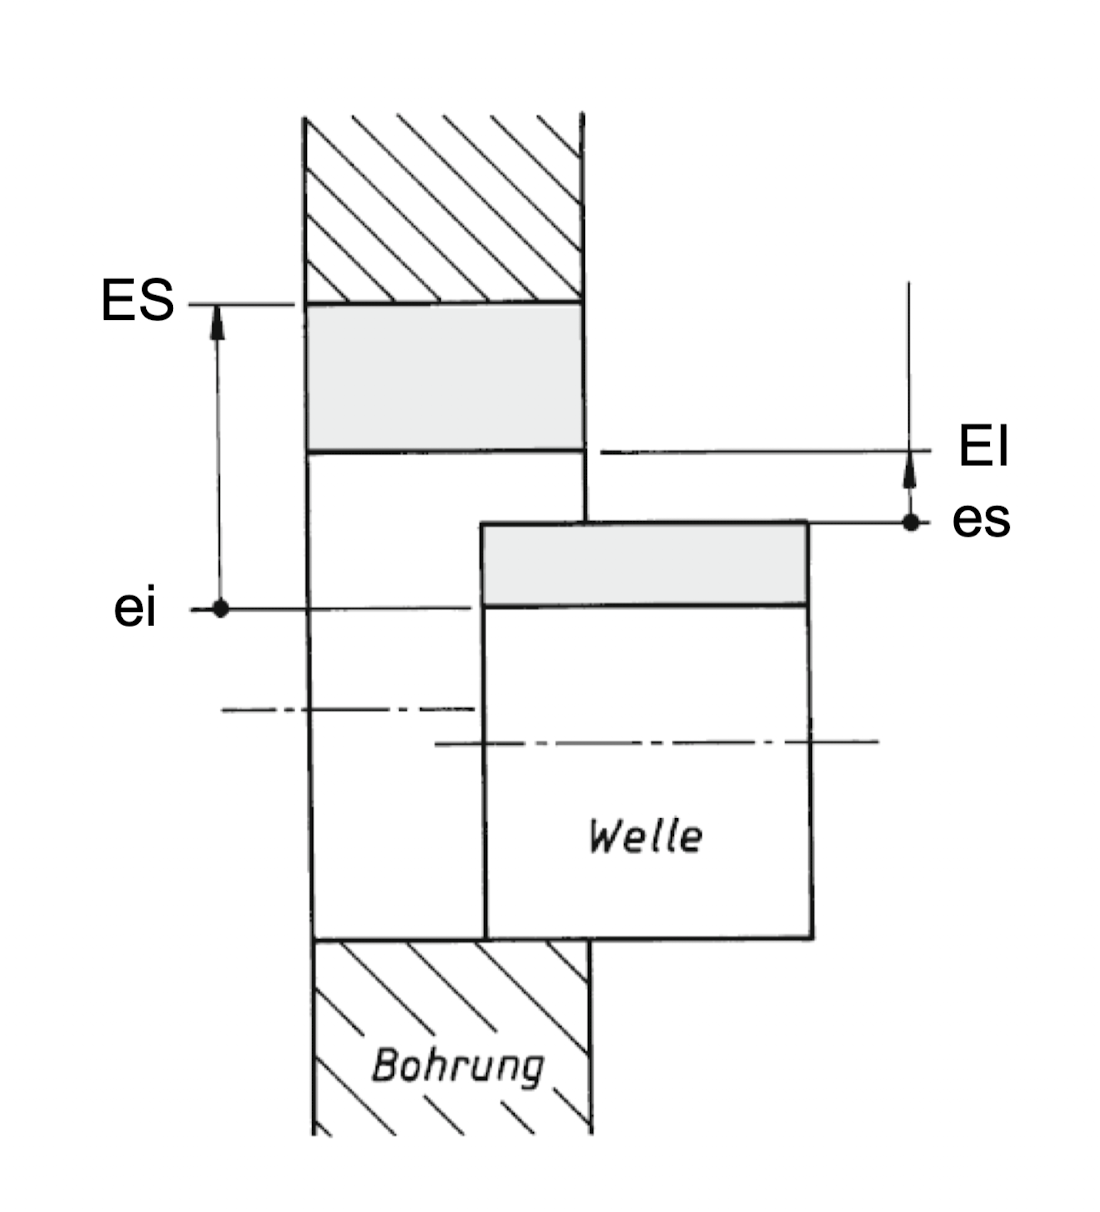
\includegraphics[width = 0.6\linewidth]{src/images/MAEIP_Spielpassung.png}
            \end{center}
        \end{minipage}
        \begin{minipage}{0.49\linewidth}
            Spielpassung
            \begin{align*}
                S_{min} &= EI - es\\
                S_{max} &= ES - ei
            \end{align*}
        \end{minipage}
    \end{minipage}
    \begin{minipage}{0.99\linewidth}
        \begin{minipage}{0.49\linewidth}
            \begin{center}
                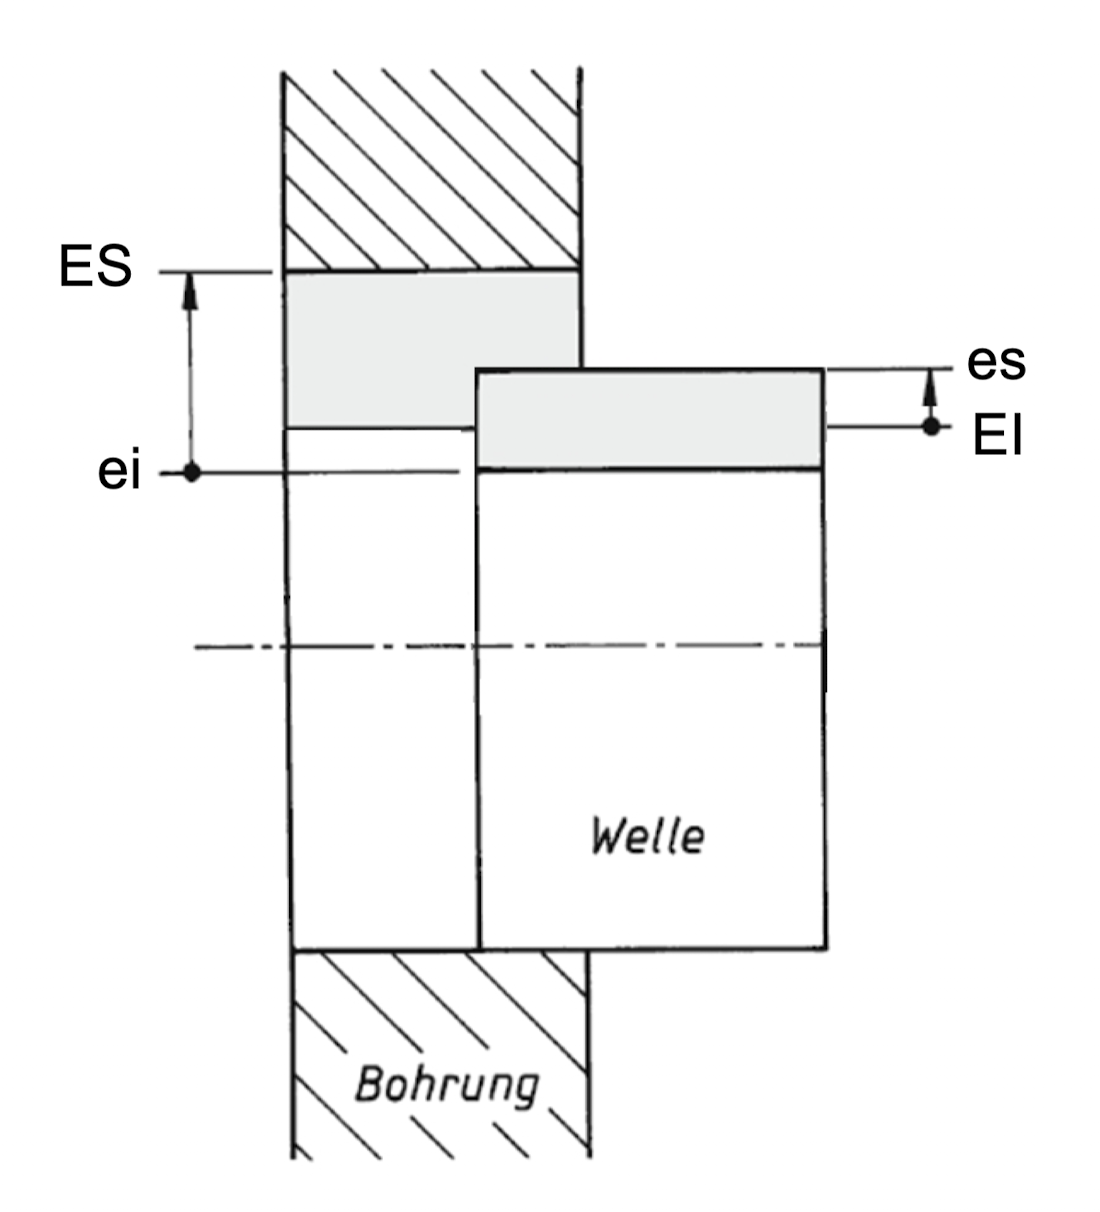
\includegraphics[width = 0.6\linewidth]{src/images/MAEIP_Uebergangspassung.png}
            \end{center}
        \end{minipage}
        \begin{minipage}{0.49\linewidth}
            Übergangspassung
        \end{minipage}
    \end{minipage}
    \begin{minipage}{0.99\linewidth}
        \begin{minipage}{0.49\linewidth}
            \begin{center}
                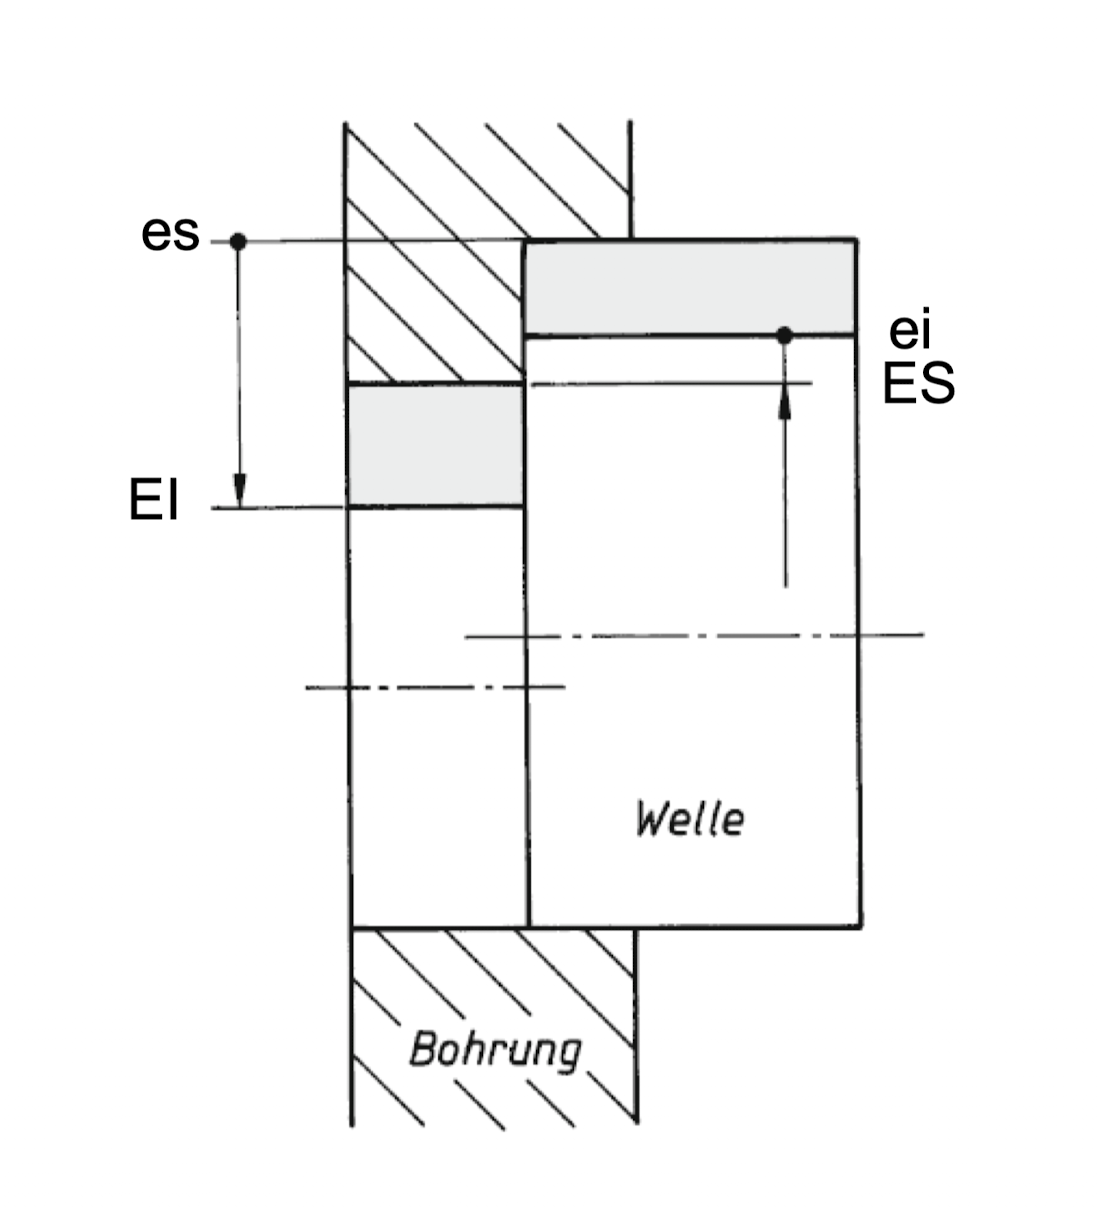
\includegraphics[width = 0.6\linewidth]{src/images/MAEIP_Uebermasspassung.png}
            \end{center}
        \end{minipage}
        \begin{minipage}{0.49\linewidth}
            Übermasspassung

            \begin{align*}
                U_{min} &= ei - ES\\
                U_{max} &= es - EI
            \end{align*}
        \end{minipage}
    \end{minipage}
    \subsection{Pressung}

\begin{align*}
    F_{R res} &= S_H \cdot \sqrt{F_l^2 + F_t^2}\\
    p_{erf} &= \frac{F_{res,max}}{\mu \cdot \pi \cdot d \cdot l_{tr}}\\
    F_{res,max} &= \sqrt{F_{t,max}^2 + F_{a,max}^2}\\
    Q_A &= \frac{D_F}{D_A}\\
    k &= 1 + \frac{1+Q_A^2}{1-Q_A^2}\\
    U_{W,min} &= \frac{p_{min} \cdot D_F}{E_A} \cdot K\\
    U_{W,max} &= \frac{p_{max} \cdot D_F}{E_A} \cdot K
\end{align*}

    \cbreak

\section{Schrauben \hfill ME}
    \begin{scriptsize}
    \begin{minipage}{0.6\linewidth}
        \begin{center}
            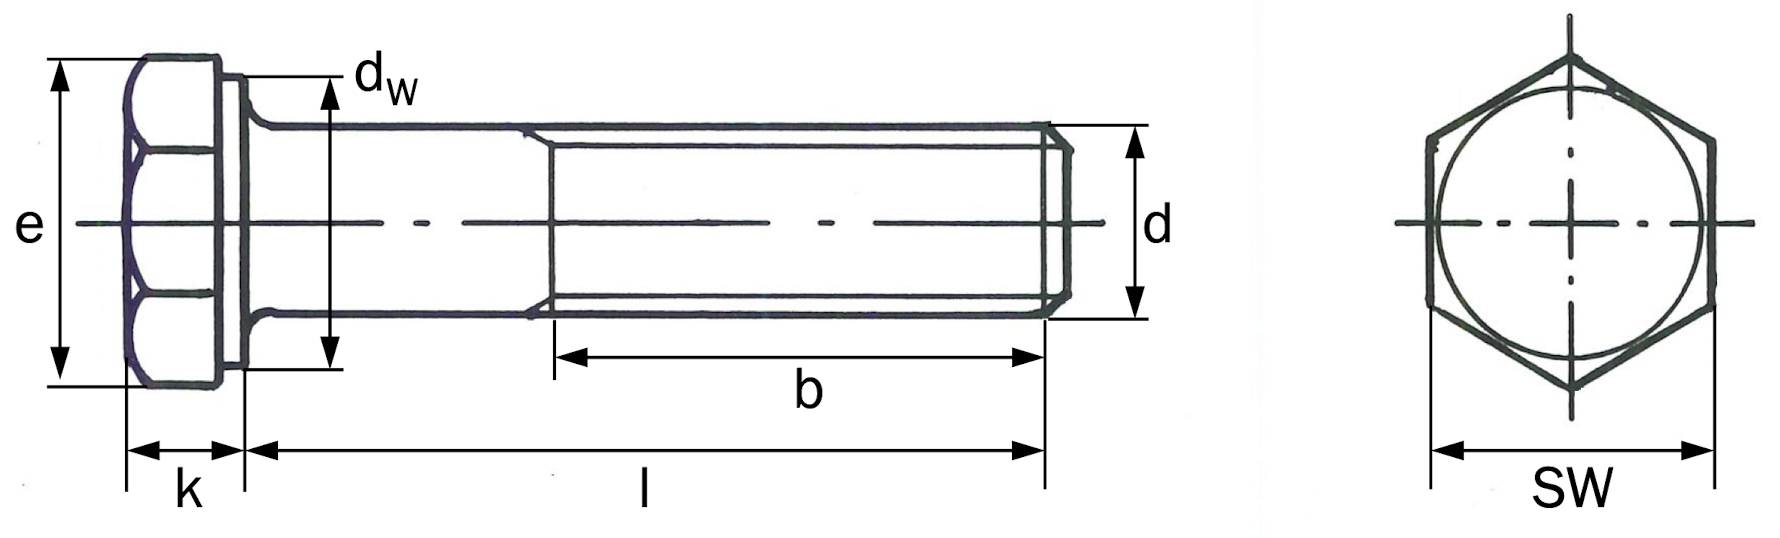
\includegraphics[width = 1.0\linewidth]{src/images/MAEIP_Schraube}
        \end{center}
    \end{minipage}
    \begin{minipage}{0.38\linewidth}
        \begin{center}
            \begin{align*}
            \text{d} &= \text{Nenndurchmesser}
            \\\text{SW} &= \text{Schlüsselweite}
            \\\text{e} &= \text{Eckmass Kopf}
            \\\text{L} &= \text{Schaftlänge}
            \\\text{b} &= \text{Gewindelänge}
            \\\text{k} &= \text{Kopfhöhe}
            \\d_w &= \text{Wirkdurchmesser}
            \end{align*}
        \end{center}
    \end{minipage}
\end{scriptsize}
    \subsection{Befestigungsgewinde \hfill ME}
\begin{minipage}{0.58\linewidth}
    \begin{center}
        \begin{scriptsize}
            \begin{tabular}{|c|c|c|}
            \hline
            \null & \cellcolor{Yellow}Metrisch & \cellcolor{Apricot}Withworth\\
            \hline
            Kurzzeichen & M & G bzw. R \\
            \hline
            Flankenwinkel $\beta$ & $60^\circ$ & $55^\circ$ \\
            \hline
            Art & Spitzgewinde & Rundgewinde \\
            \hline
            Anwendung & Universell & Rohrleitung\\
            \hline
        \end{tabular}
        \end{scriptsize}
    \end{center}
\end{minipage}
\begin{minipage}{0.4\linewidth}
    \begin{center}
        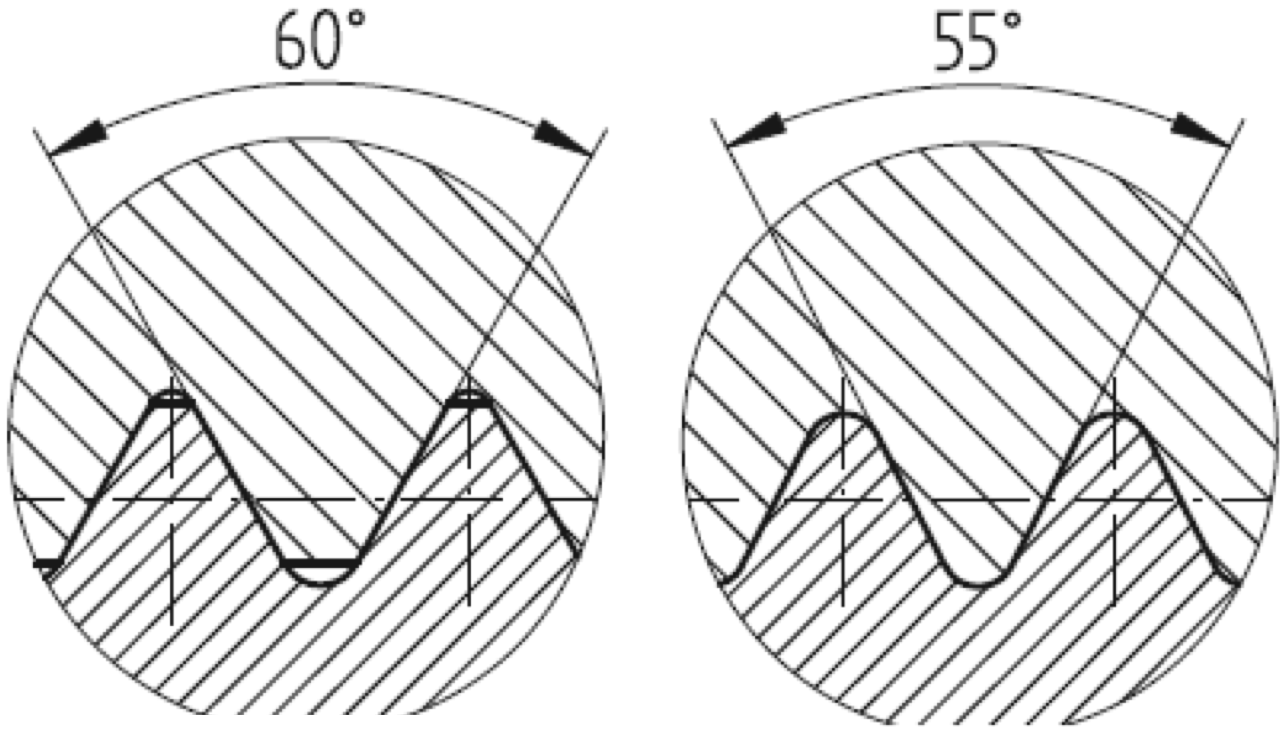
\includegraphics[width = 0.9\linewidth]{src/images/MAEIP_BG}
    \end{center}
\end{minipage}
    \subsection{Bewegungsgewinde \hfill ME}
\begin{minipage}{0.58\linewidth}
    \begin{center}
        \begin{scriptsize}
            \begin{tabular}{|c|c|c|}
            \hline
            \null & \cellcolor{LimeGreen}Trapez & \cellcolor{GreenYellow}Sägen\\
            \hline
            Kurzzeichen & Tr & S \\
            \hline
            Flankenwinkel $\beta$ & $30^\circ$ & $30^\circ / 3^\circ$\\
            \hline
            Anwendung & Handrad & \thead{\scriptsize Hydraulische \\\scriptsize Presse}\\
            \hline
        \end{tabular}
        \end{scriptsize}
    \end{center}
\end{minipage}
\begin{minipage}{0.4\linewidth}
    \begin{center}
        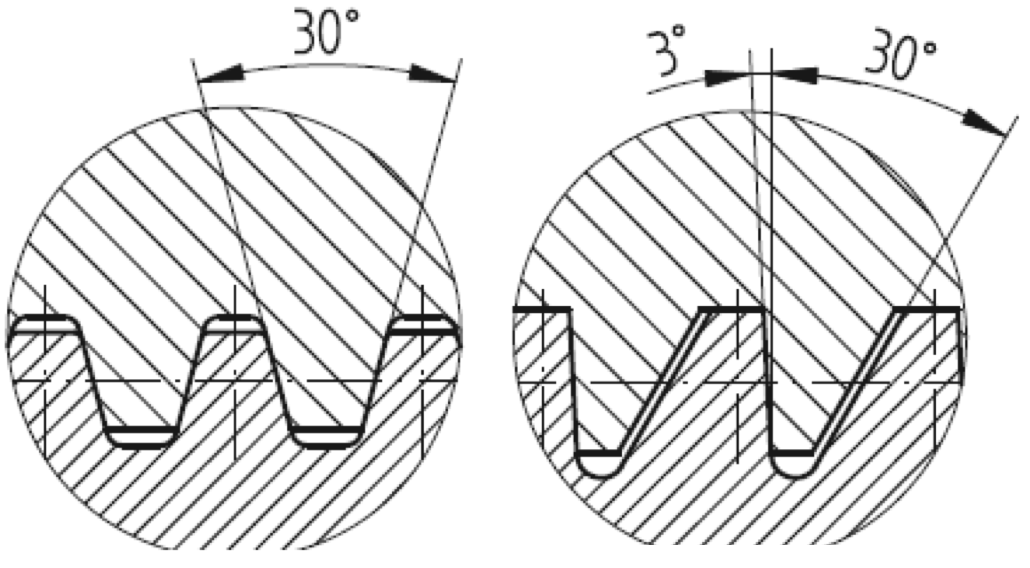
\includegraphics[width = 0.9\linewidth]{src/images/MAEIP_BewG}
    \end{center}
\end{minipage}
    \subsection{Gewindesteigung \hfill ME}
\begin{footnotesize}
    \begin{itemize}
        \item $P$ = Gewindesteigung = Zurückgelegter Weg bei einer Umdrehung
        \item Bsp.: M30 x 2 $\to$ $d = 30, P = 2$ (P angegeben $\rightarrow$ Feingewinde)
    \end{itemize}
    \begin{minipage}{0.58\linewidth}
        \begin{center}
            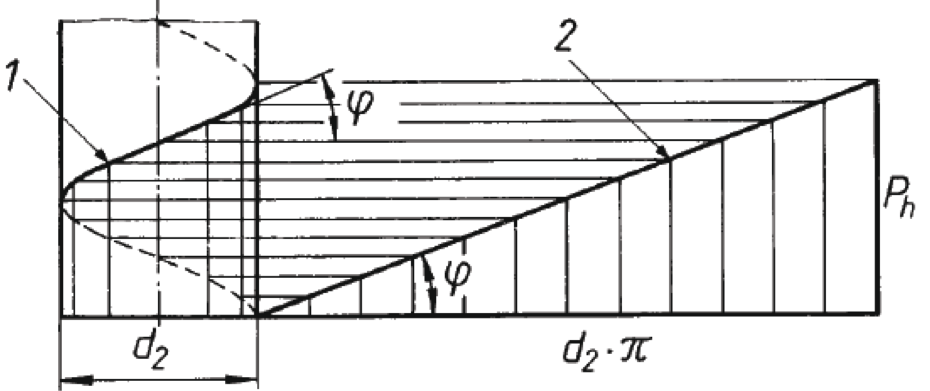
\includegraphics[width = 0.8\linewidth]{src/images/MAEIP_Gewindesteigung}
            \mathbox{
                tan(\varphi) = \frac{P}{2\pi \cdot r_m} = \frac{P}{\pi \cdot d_2}
            }
        \end{center}
    \end{minipage}
    \begin{minipage}{0.4\linewidth}
        \begin{center}
            \begin{align*}
                \varphi &= \text{Steigungswinkel}
                \\ P &= \text{Gewindesteigung}
                \\ d_2 &= \text{Flankendurchmesser}
            \end{align*}
            \mathbox{
                P = \frac{\text{eingeschraubte Distanz}}{\# \text{Umdrehungen}}
            }
        \end{center}
    \end{minipage}
    \begin{empheq}[box=\fbox]{align*}
        &\text{Regelsteigung (wenn bei Deklaration keine Angabe steht): }\\
        &P = 1.75 mm \text{ Abhängig von Schraubendurchmesser}
    \end{empheq}
\end{footnotesize}

    \subsection{Schraubenquerschnitte \hfill ME}
\begin{footnotesize}
    \begin{minipage}{0.55\linewidth}
        \begin{center}
            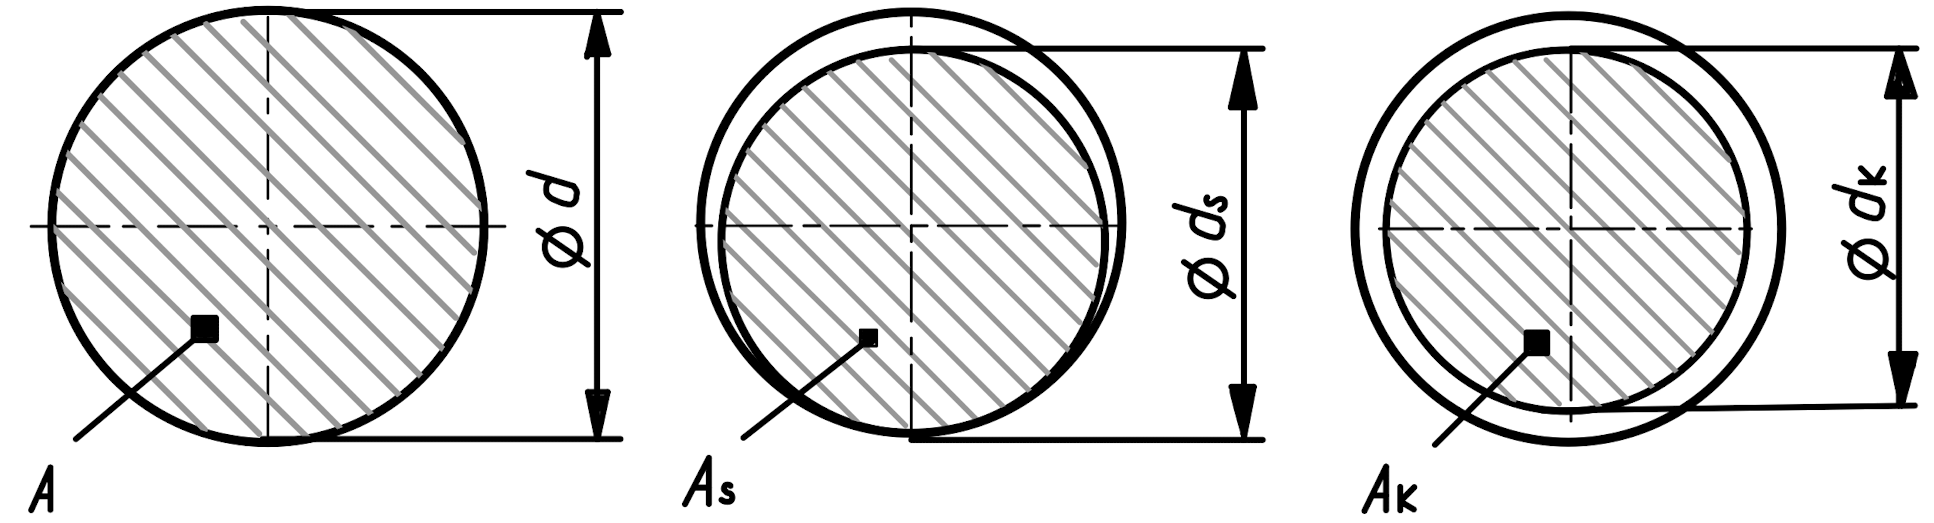
\includegraphics[width = 0.9\linewidth]{src/images/MAEIP_Schraubenquerschnitte}
            \mathbox{
                d_s = \frac{1}{2} \cdot (d_2 + d_3)
            }
        \end{center}
    \end{minipage}
\end{footnotesize}
    \begin{minipage}{0.4\linewidth}
        \begin{scriptsize}
        \begin{center}
            \begin{align*}
                d &= \text{Nenndurchmesser} [d_2]
                \\d_s &= \text{Spannungsdurchmesser}
                \\d_k &= \text{Kerndurchmesser} [d_3]
                \\A &= \text{Schaftquerschnitt} [A_2]
                \\A_s &= \text{Spannungsquerschnitt}
                \\A_k &= \text{Kernquerschnitt} [A_3]
            \end{align*}
        \end{center}
    \end{scriptsize}
    \end{minipage}
    \subsection{Schraubenköpfe \hfill ME}
\begin{footnotesize}
    \begin{center}
        \begin{tabular}{|c|c|c|c|}
            \hline
            \null & Anziehmoment & Preis & Werkzeug\\
            \hline
            Schlitz & $\downarrow$ & $\downarrow$$\downarrow$ & schlechte Zentrierung\\
            \hline
            Kreuz & $\downarrow$ & $\downarrow$$\downarrow$ & gute Zentrierung\\
            \hline
            Aussensechs. & $\uparrow$ & $\downarrow$ & grosser Platzbedarf\\
            \hline
            Imbus & $\to$ & $\downarrow$ & geringer Platzbedarf\\
            \hline
            Aussenvielzahn. & $\uparrow \uparrow$ & $\uparrow$ & grosser Platzbedarf\\
            \hline
            Torx & $\uparrow$ & $\uparrow$ & geringer Platzbedarf\\
            \hline
          \end{tabular}
    \end{center}
\end{footnotesize}
    \subsection{Festigkeitsklassen \hfill ME}
\begin{footnotesize}
    Zugfestigkeit: Versagen des Materials, Streckgrenze: elastische Verformung
    \begin{center}
        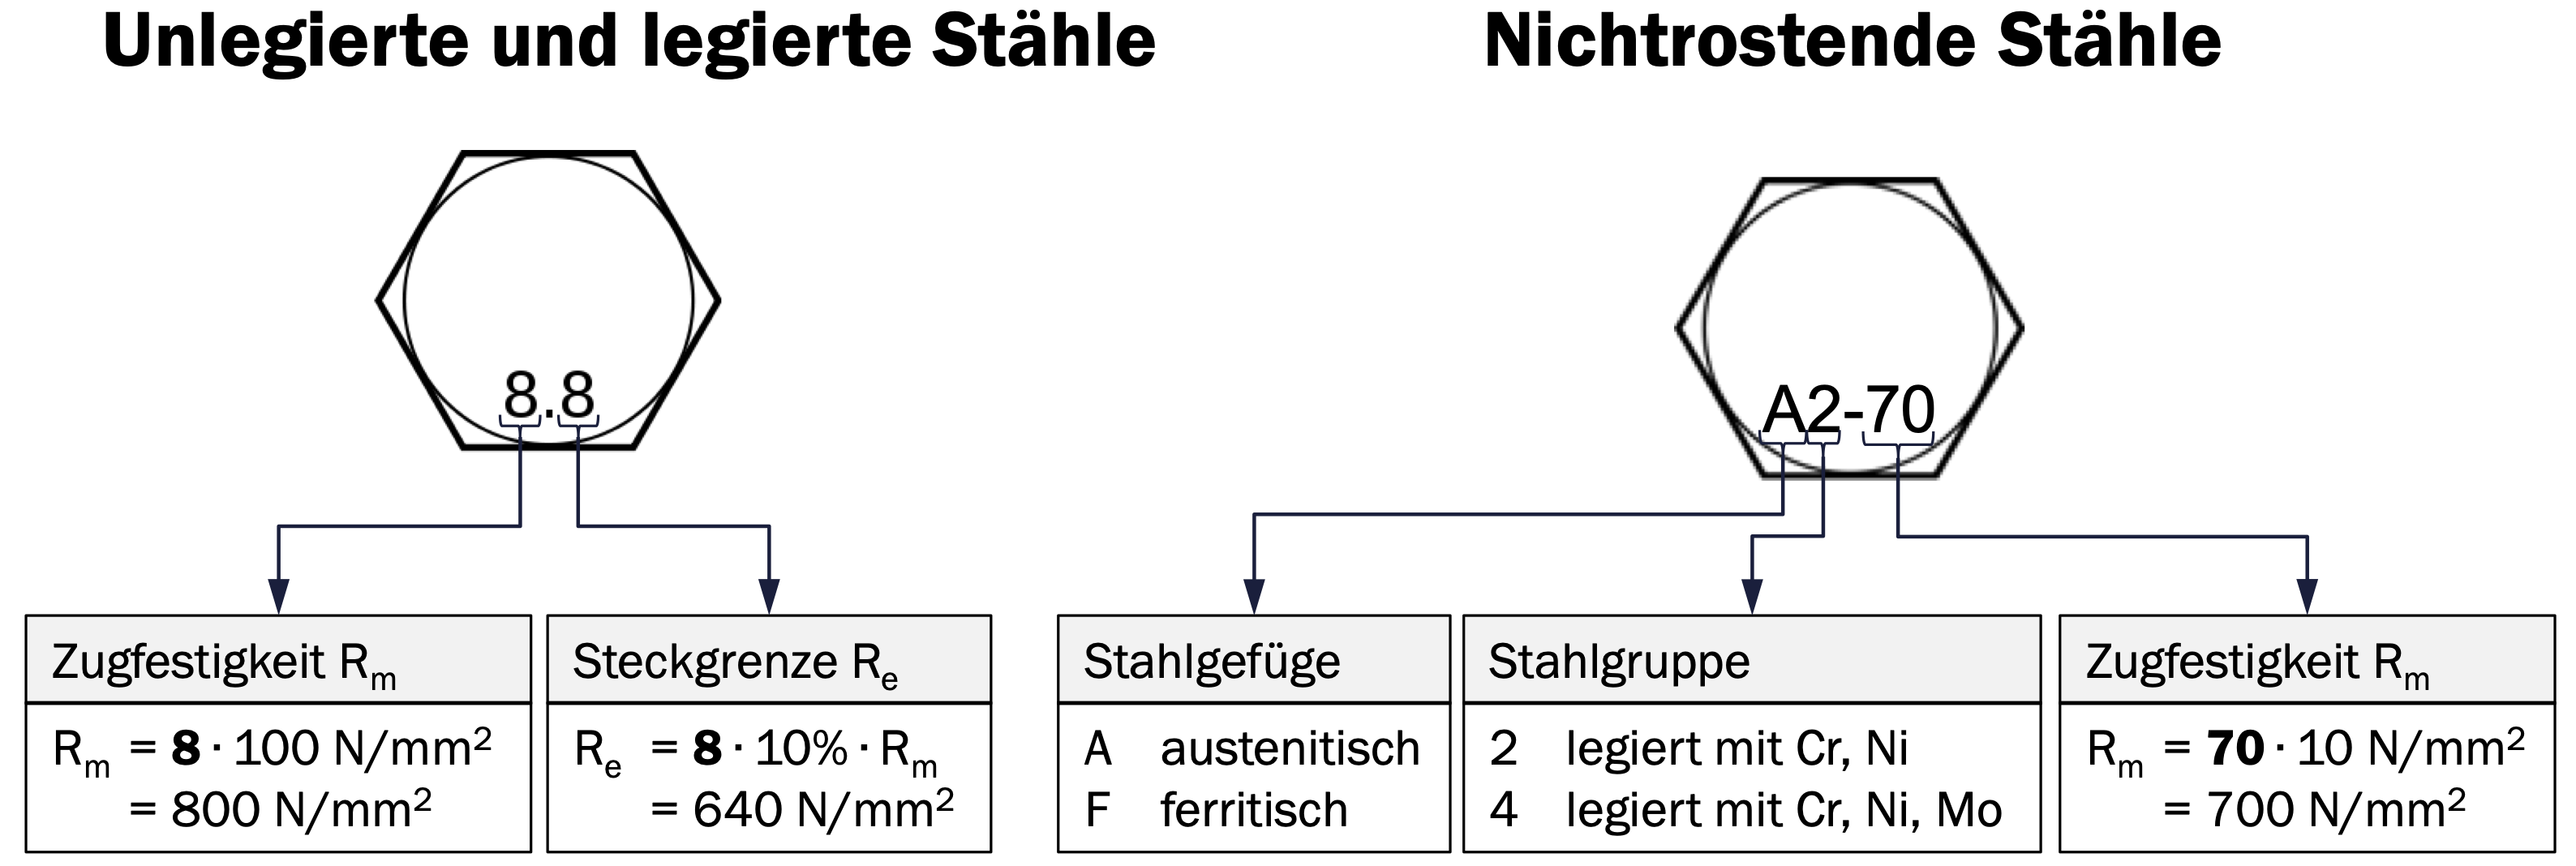
\includegraphics[width = 1.0\linewidth]{src/images/MAEIP_Festigkeitsklassen}
    \end{center}
\end{footnotesize}
\cbreak
    \subsection{Belastung Schraube \hfill ME}
\begin{footnotesize}
    \begin{center}
        \begin{empheq}[box=\fbox]{align*}
            \sigma_z &= \frac{F_{s, \text{max}}}{A_s} \quad \mid \quad \tau_t = \frac{M_{t, \text{max}}}{W_{t,3}} \quad \mid \quad W_{t,3} = \frac{\pi d_3^3}{16}
            \\M_A &= M_G + M_K \quad \mid \quad \tan(\rho) = \frac{\mu_G}{cos(\frac{\beta}{2})}
            \\M_{G,\text{max}} &= F_{\textrm{VM}} \frac{d_2}{2} \tan(\varphi + \rho) \quad \mid \quad M_K = F_{\textrm{VM}}\cdot \mu_K\frac{D_{km}}{2}
        \end{empheq}
        \begin{empheq}[box=\fbox]{align*}
            \text{Für metrische}\: \text{Regelgewinde} \:&\text{mit mittleren Reibungszahlen:}
            \\M_A \approx 0.17 &\cdot F_{\textrm{VM}} \cdot d
        \end{empheq}
    \end{center}
    \begin{scriptsize}
        \begin{center}
            $F_{s, \text{max}}$ = Schraubenkraft; $A_s$ = Spannungsquerschnitt;
            \\$M_{M, \text{max}}$ = Montagemoment; $M_A$ = Anziehmoment; $\sigma_z$ = Zugspannung;
            \\$F_{\textrm{VM}}$ = Vorspannkraft; $\rho$ = Reibungswinkel; $\tau_t$ = Torsionsspannung
    \end{center}
    \end{scriptsize}
\end{footnotesize}
    \subsection{Schraube als Feder \hfill ME}
\begin{footnotesize}
    \begin{empheq}[box=\fbox]{align*}
        F_v &= \frac{1}{\delta_S} \cdot f_S = \frac{1}{\delta_p} \cdot f_p \quad \mid \quad \quad \delta = \frac{l}{E\cdot A}
        \\ f &= \varepsilon \cdot l = \frac{\sigma}{E}\cdot l = \frac{F}{E\cdot A}\cdot l
        \\ & \text{ \textcolor{Red}{ $A$ Abhängig von Schraubenabschnitt}}
    \end{empheq}
    \begin{scriptsize}
        $F$ = aufgebrachte Zugkraft; $\delta$ = Nachgiebigkeit; $f$ = elastische Längenänderung; 
        \\$E$ = E-Modul; $A$ = Querschnittsfläche; $l$ = Länge beliebiges Material; 
        \\$\sigma$ = Zugspannung im Material; $\varepsilon$ = Dehnung in Belastungsrichtung
    \end{scriptsize}
\end{footnotesize}
\vspace{2mm}
    \subsection{Schraubenkraft $F_S$ $\mid$ Restklemmkraft $F_K$ \hfill ME}
\begin{footnotesize}
    \begin{itemize}
        \scriptsize{\item $F_S$ = Summe aller Kräfte, die auf Schub wirken: }
        \vspace{-2mm}  
        \mathbox{
            F_S > F_{S,\text{zul}} \Rightarrow \text{Versagen}
        }
        \vspace{-3mm}
        \scriptsize{\item $F_K$ = Kraft, mit der die Platten im Betrieb noch gehalten werden}
        \vspace{-2mm}
        \mathbox{
            F_K < F_{K, \text{erf}} \Rightarrow \text{Versagen}
        }
    \end{itemize}
\end{footnotesize}
    \subsection{Schraubenauslegung \hfill ME}
\begin{footnotesize}
    \begin{minipage}{0.49\linewidth}
        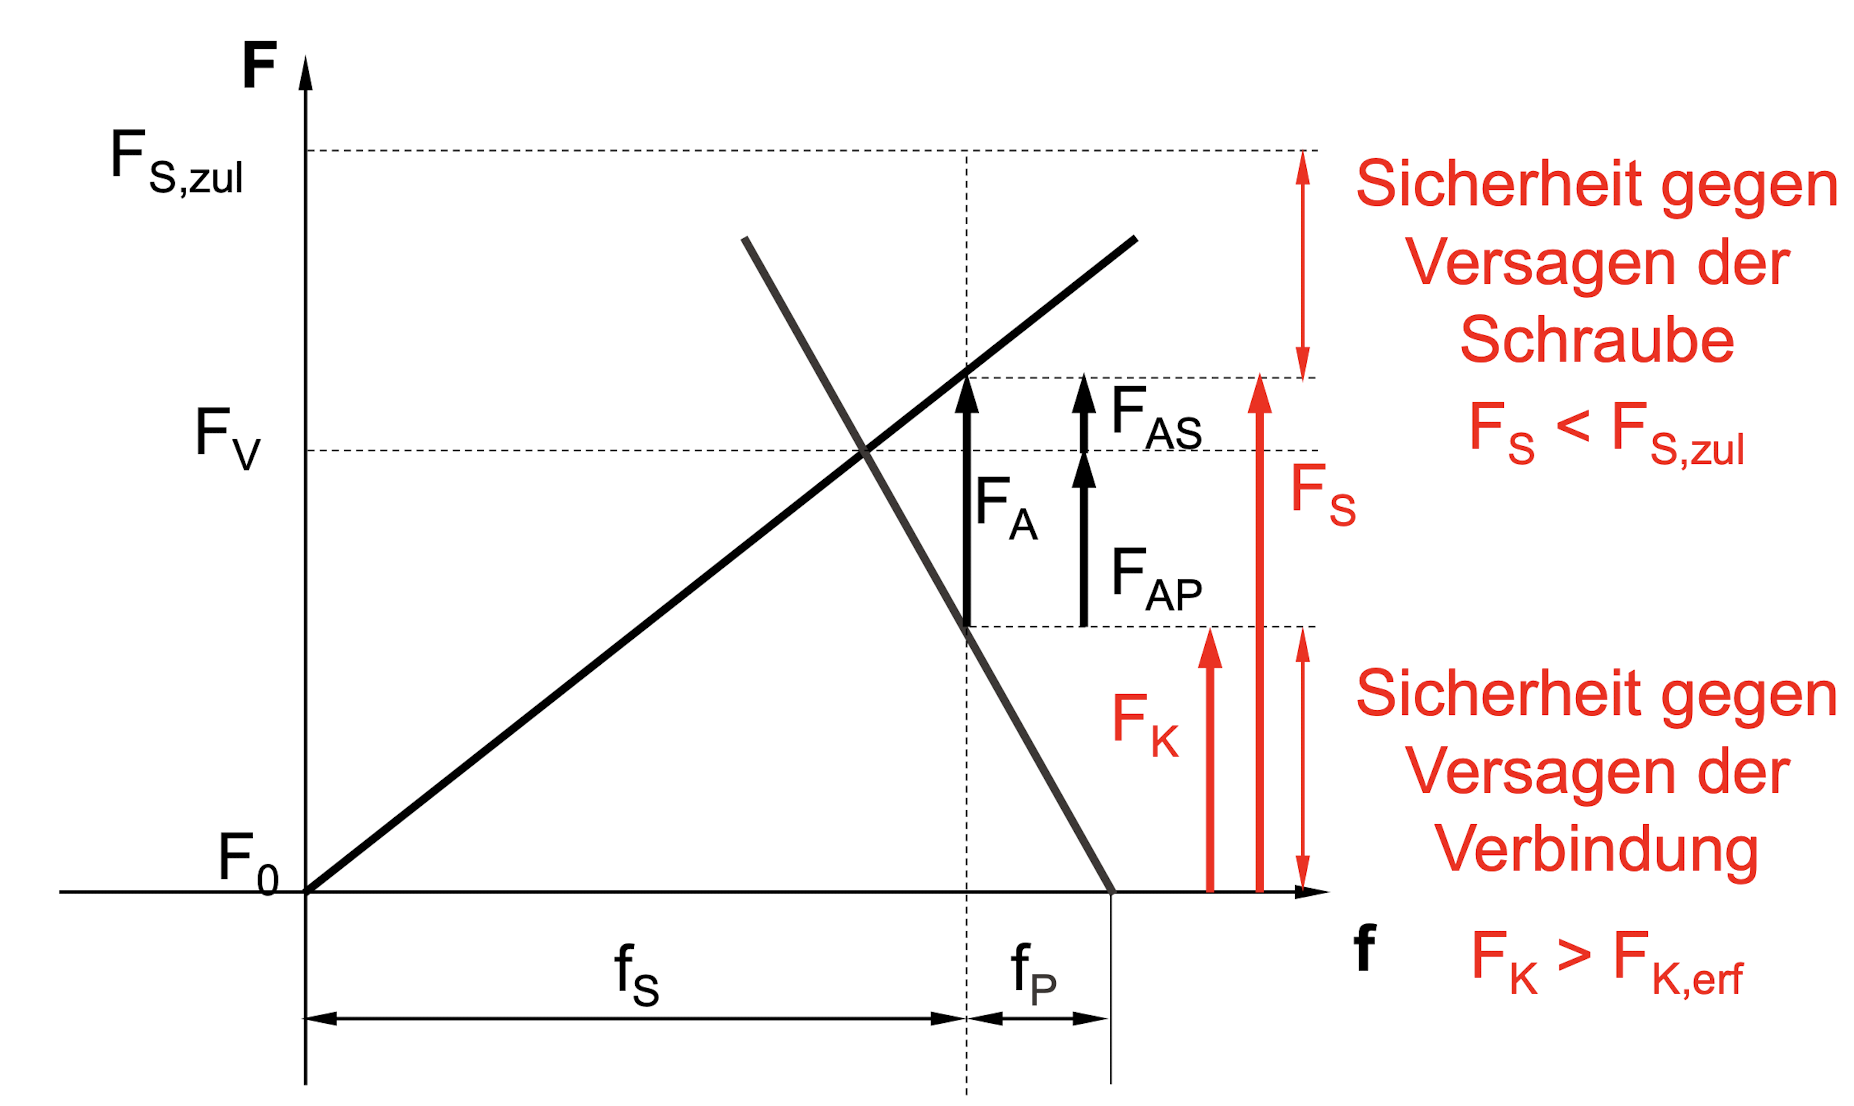
\includegraphics[width = 1.0\linewidth]{src/images/MAEIP_Schraubenauslegung1}
    \end{minipage}
    \begin{minipage}{0.49\linewidth}
        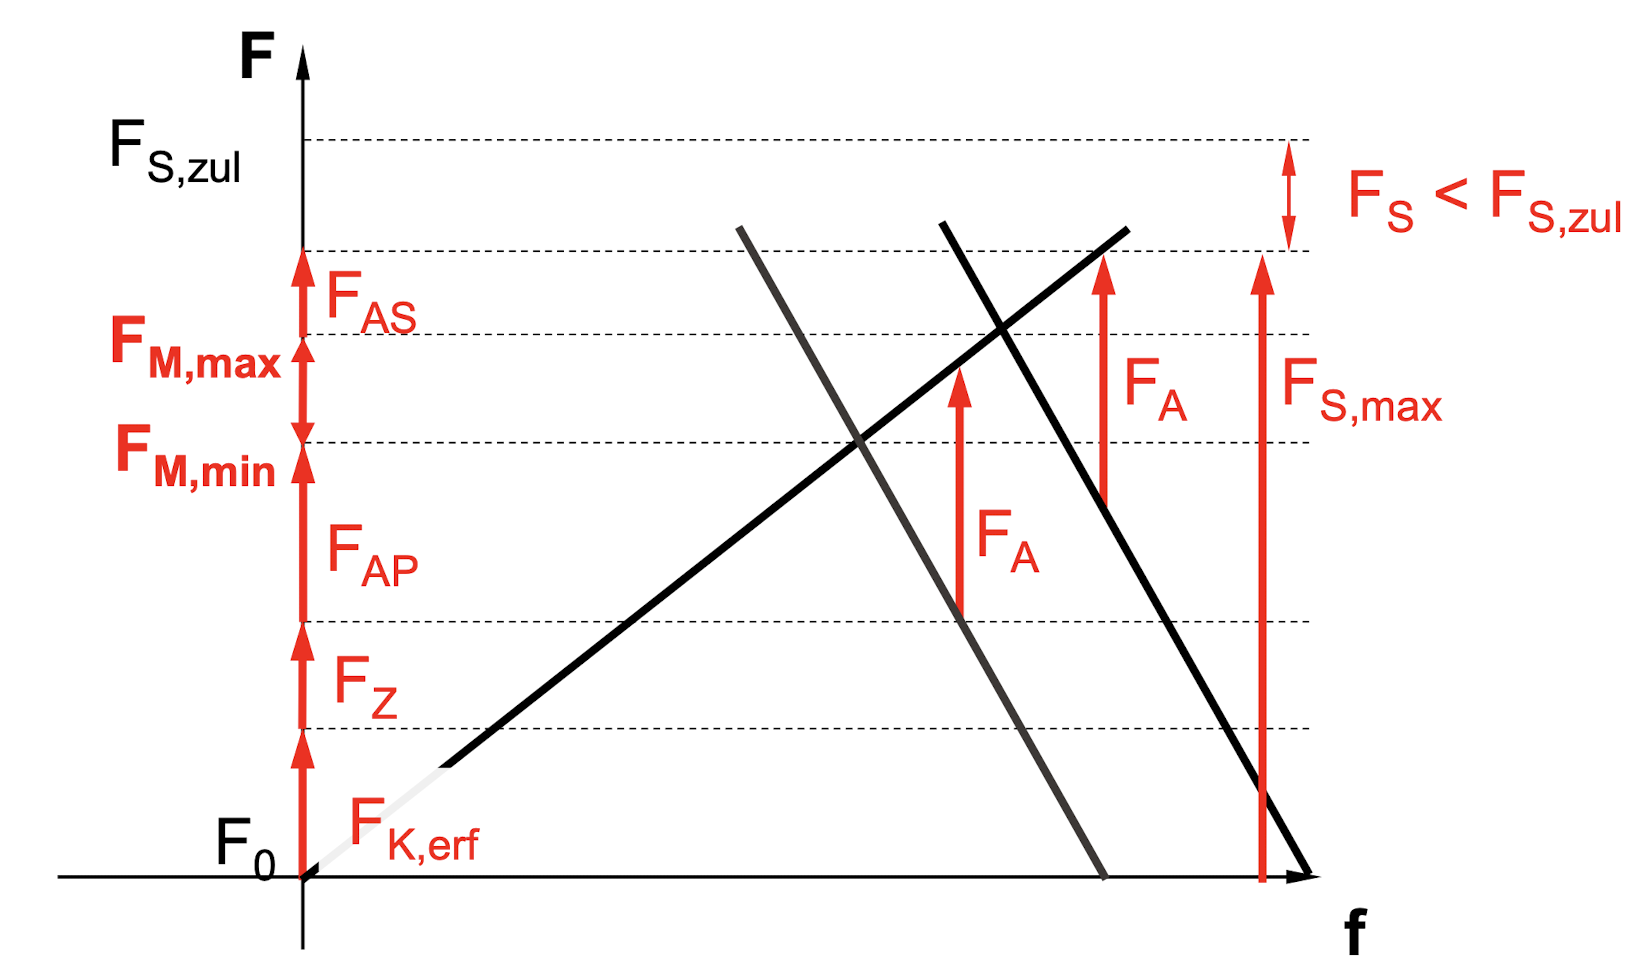
\includegraphics[width = 1.0\linewidth]{src/images/MAEIP_Schraubenauslegung2}
    \end{minipage}
    \begin{empheq}[box=\fbox]{align*}
        \scriptstyle F_{V, \text{min}} = F_{Kl, \text{erf}} + F_{BT} + F_Z \quad \mid \quad \sigma_V = \sqrt{\sigma_z^2 + 3 \cdot \tau_t^2}
        \\F_{V, \text{max}} = k_A \cdot F_{V, \text{min}} \quad \mid \quad F_{S, \text{max}} = F_{V, \text{max}} + F_{BS}
        \\ \scriptstyle F_{BS} = \frac{\delta_T}{\delta_S + \delta_T} F_B \quad \mid \quad F_{BT} = \frac{\delta_S}{\delta_S + \delta_T} F_B
        \\ \Delta f = F_BS \delta_S = F_{BT} \delta_T \quad \mid \quad F_Z = \frac{f_Z}{\delta_S + \delta_T}
    \end{empheq}
    \begin{scriptsize}
        \begin{minipage}{0.53\linewidth}
            \begin{empheq}[box=\fbox]{align*}
                F_{V, \text{min}} &= \text{Min. Anziehkraft}
                \\F_{BT}, F_{BS} &= \text{Axiale Betriebslast}
                \\&\text{ auf Platten / Schrauben}
                \\F_{V, \text{max}} &= \text{Max. Anziehkraft}
                \\\sigma_z &= \text{Max. Zugspannung}
                \\R_e &= \text{Streckgrenze}
            \end{empheq}
        \end{minipage}
        \begin{minipage}{0.45\linewidth}
            \begin{empheq}[box=\fbox]{align*}
                F_{Kl, \text{erf}} &= \text{erf. Klemmkraft}
                \\F_Z &= \text{Setzkraftverlust}
                \\k_A &= \text{Anziehfaktor}
                \\\tau_t &= \text{Max. Schubspannung}
                \\\sigma_V &= \text{Max. Vergleichsp.}
            \end{empheq}
        \end{minipage}
    \end{scriptsize}    
\end{footnotesize}
    \subsection{Nachgiebigkeit Schraube \hfill ME}
\begin{empheq}[box=\fbox]{align*}
    \scriptstyle \delta_s = \frac{1}{E_s}\left( \frac{l_{ko}}{A_N} + \frac{l_1}{A_{d1}} + \frac{l_2}{A_{d2}} + \frac{l_i}{A_{di}} + \frac{l_G}{A_3} + \frac{l_{\text{Ge}}}{A_3}  \right) + \frac{l_M}{E_M \cdot A_N}
\end{empheq}
\begin{minipage}{0.4\linewidth}
    \begin{center}
        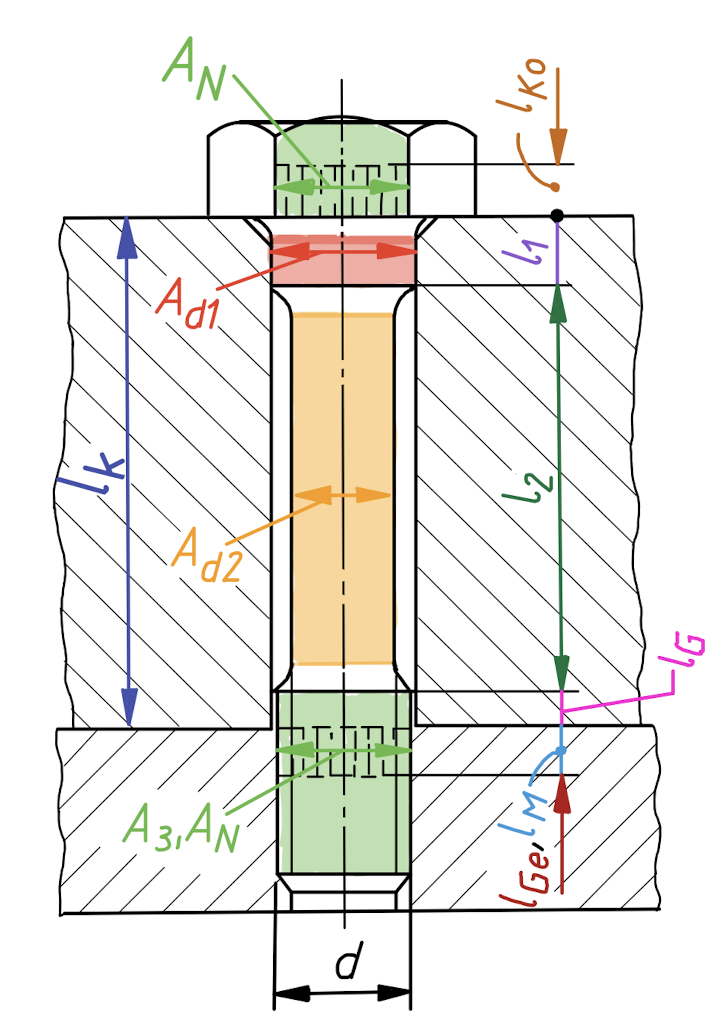
\includegraphics[width= 0.9\linewidth]{src/images/MAEIP_NachgiebigkeitSchraube}
    \end{center}
\end{minipage}
\begin{minipage}{0.58\linewidth}
    \begin{center}
        \begin{scriptsize}
            \begin{empheq}[box=\fbox]{align*}
                A_N = A_2 &= \text{Kopf / Mutter}
                \\A_2 &= \text{Schaft} 
                \\A_3 &= \text{Gewinde}
            \end{empheq}
            \begin{tabular}{|c|c|}
                \hline
                Sechskant & $l_{k0}= 0.5d$\\
                \hline
                Innensechskant & $l_{k0} = 0.4d$\\
                \hline
                \thead{\scriptsize eingeschraubtes \\ \scriptsize Gewinde} & $l_{Ge} = 0.5d$\\
                \hline
                Schraubenmutter & $l_M = 0.4d$\\
                \hline
                Einschraubgewindebereich & $l_M= 0.33d$\\
                \hline
            \end{tabular}
        \end{scriptsize}
    \end{center}
\end{minipage}

\subsection{Nachgiebigkeit Platte \hfill ME}
\begin{empheq}[box=\fbox]{align*}
    \scriptstyle A_{ers} = \frac{\pi}{4} \left(d_w^2 - d_h^2\right) + \frac{\pi}{8} \cdot d_w \cdot \left(D_A - d_w\right) \cdot \left(\left(x + 1\right)^2 - 1\right)
\end{empheq}
\begin{minipage}{0.4\linewidth}
    \begin{center}
        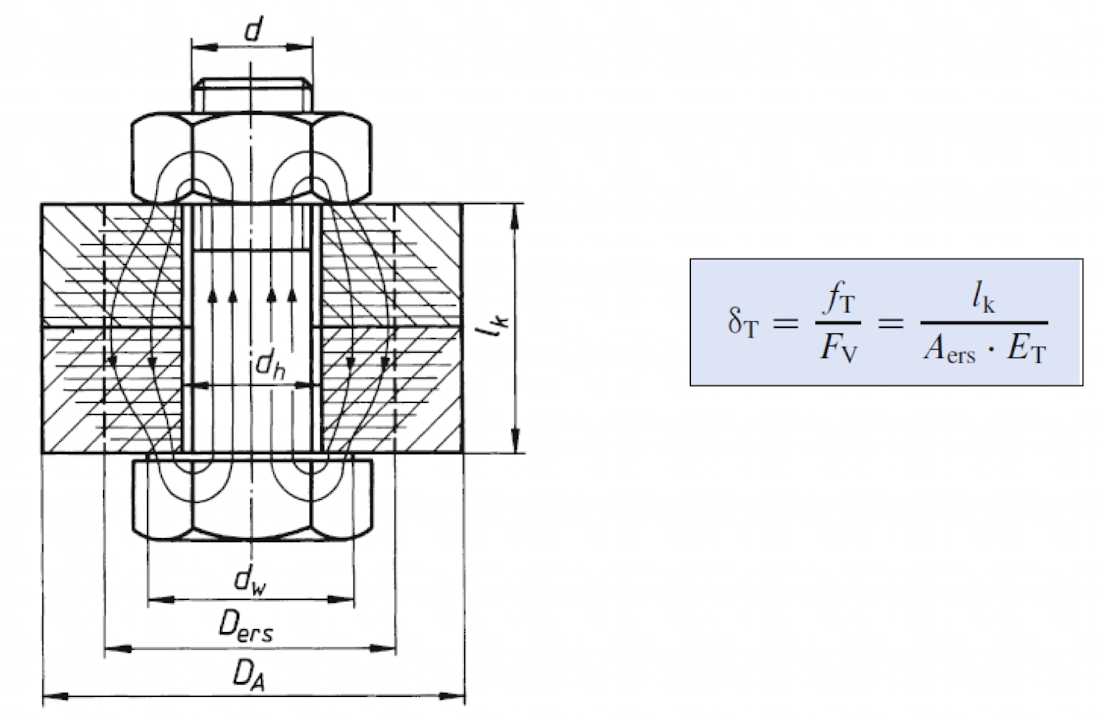
\includegraphics[width= 1\linewidth]{src/images/MAEIP_NachgiebigkeitPlatte}
    \end{center}
\end{minipage}
\begin{minipage}{0.58\linewidth}
    \begin{center}
        \begin{scriptsize}
            \begin{empheq}[box=\fbox]{align*}
                x &= \sqrt[3]{\frac{l_k \cdot d_w}{D_A}}
                \\ \delta_T &= \frac{f_T}{F_V} = \frac{l_k}{A_{ers} \cdot E_T}
            \end{empheq}
        \end{scriptsize}
    \end{center}
\end{minipage}
    \subsection{Anziehverfahren}
\begin{itemize}
    \item Anziehen mit Längungssteuerung bzw. -kontrolle per Ultraschall\\
    \item Hydraulisches Anziehen\\
    \item Streckgrenzgesteuertes oder drehwinkelgesteuertes Anziehen (von Hand oder motorisch)\\
    \item Impulsschrauber mit hydraulischer Pulszelle, drehmoment- und/oder drehwinkelgesteuert\\
    \item Drehmomentgesteuertes Anziehen mit Drehmoment-schlüssel, signalgebendem Schlüssel oder motorischem Drehschrauber mit dynamischer Drehmomentmessung\\
    \item Anzichen mit Schlagschrauber; "Abwürgschrauber" oder Impulsschrauber; Anziehen von Hand
\end{itemize}

\section{Federn \hfill ME}
    \subsection{Schraubenfeder \hfill ME}
    \begin{center}
        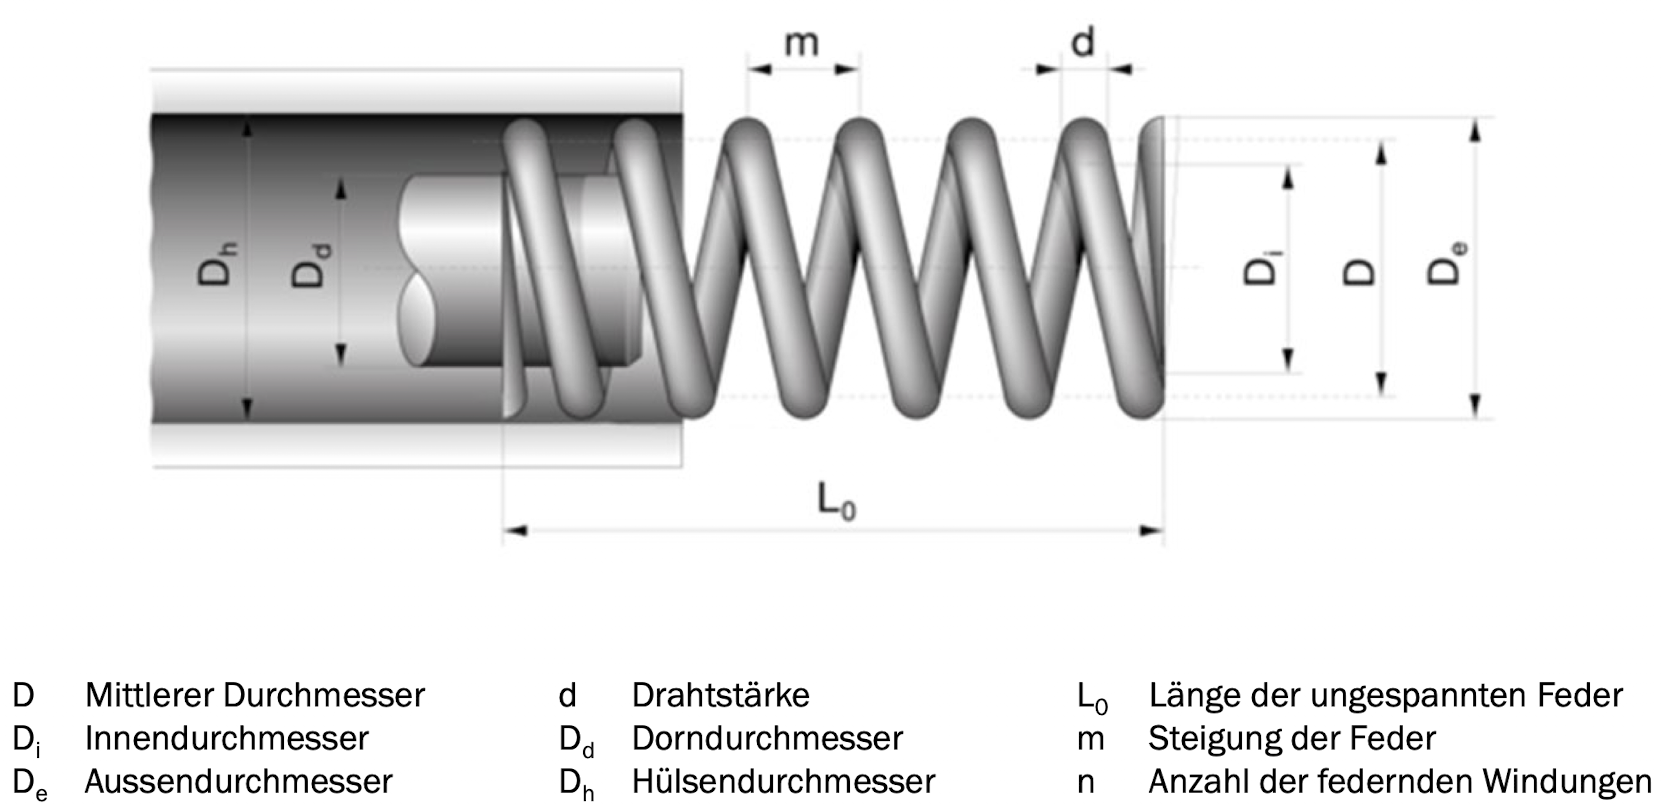
\includegraphics[width = 0.8\linewidth]{src/images/MAEIP_Schraubenfeder}

    \end{center}
    \begin{minipage}{0.57\linewidth}
        \begin{footnotesize}
            \begin{empheq}[box = \fbox]{align*}
                R &= \frac{G \cdot d^4}{8 \cdot D^3 \cdot n}
                \\F &= R \cdot s
                \\W &= \frac{1}{2} \cdot R (s_2^2 -s_1^2) \: [\text{Nmm}]
                \\ &= \frac{1}{2} \cdot (F_2s_2 - F_1s_1)
                \\\tau_t &= G \cdot tan(\gamma)
                \\ D&= D_e -d
            \end{empheq}
        \end{footnotesize}
    \end{minipage}
    \begin{minipage}{0.41\linewidth}
        \begin{scriptsize}
            \begin{empheq}[box= \fbox]{align*}
                R &= \text{Federrate}
                \\ G&= \text{Schubmodul}
                \\ \tau_t &= \text{Torsionsspannung}
                \\W &= \text{Federarbeit}
                \\\gamma &= \text{Verdrehwinkel}
                \\ n &= \text{\# federnde Windungen}
            \end{empheq}
        \end{scriptsize}
    \end{minipage}
    \subsection{Parallel vs. Reihenschaltung \hfill ME}
\begin{footnotesize}
    \begin{center}
        \begin{minipage}{0.5\linewidth}
            \begin{empheq}[box = \fbox]{align*}
                &\text{Parallelschaltung:}
                \\F &= F_1 + F_2 + F_3
                \\s_1 &= s_2 = s_3 = s
                \\R_{\text{ers}} &= R_1 + R_2 + R_3
            \end{empheq}
        \end{minipage}
        \begin{minipage}{0.48\linewidth}
            \begin{empheq}[box= \fbox]{align*}
                &\text{Reihenschaltung:}
                \\s &= s_1+s_2+s_3
                \\F &= F_1+F_2+F_3
                \\R_{\text{ers}} &= \frac{1}{\frac{1}{R_1}+\frac{1}{R_2}+\frac{1}{R_3}}
            \end{empheq}
        \end{minipage}
            \begin{empheq}[box=\fbox]{align*}
                &\text{Kombiniert (zuerst Parallel-, dann Reihenschaltungen):} 
                \\ &R = \frac{1}{\frac{1}{R_1+R_2} + \frac{1}{R_3 + R_4}}
            \end{empheq}
    \end{center}    
\end{footnotesize}
    \subsection{Kennlinien \hfill ME}
\begin{footnotesize}
    \begin{center}
        \begin{minipage}{0.58\linewidth}
            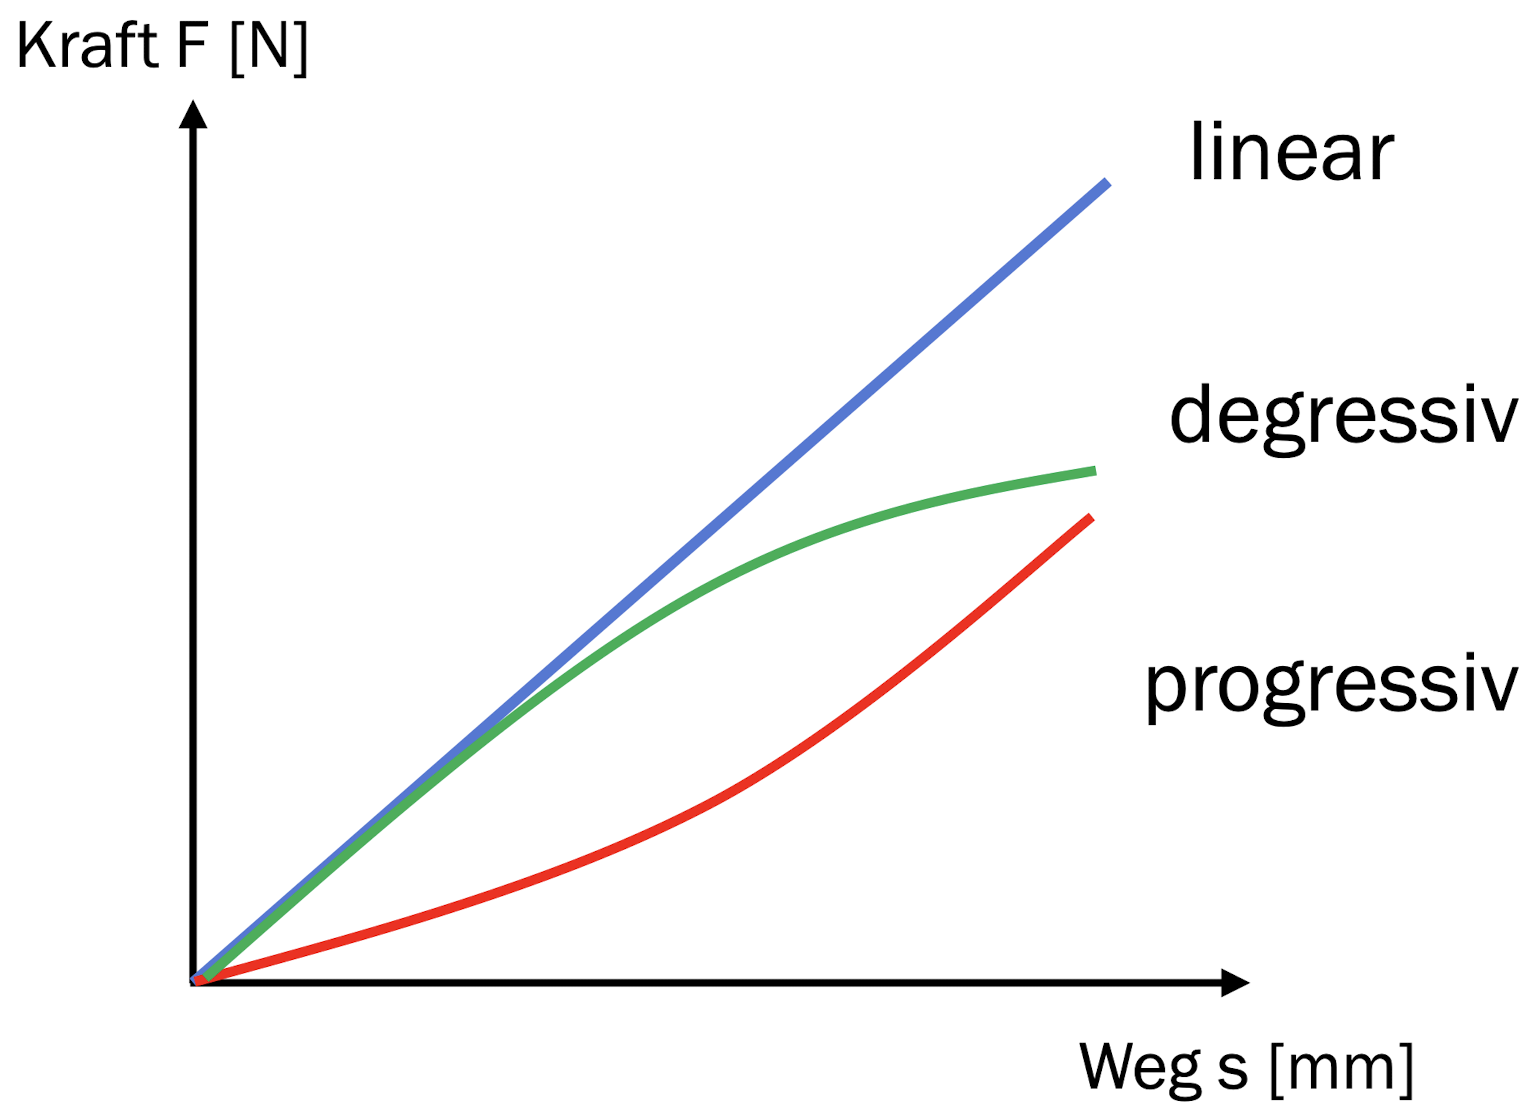
\includegraphics[width = 0.7\linewidth]{src/images/MAEIP_Kennlinien}
        \end{minipage}
        \begin{minipage}{0.4\linewidth}
            \textbf{Progressiv:} wird härter
            \\$\to$ Fahrzeugfederung
            \\~\\
            \textbf{Degressiv:} wird weicher
            \\$\to$ Verschleissausgleich bei\\ Kupplung
        \end{minipage}
    \end{center}
\end{footnotesize}
    \subsection{Tellerfedern \hfill ME}
\begin{footnotesize}
    \begin{center}
        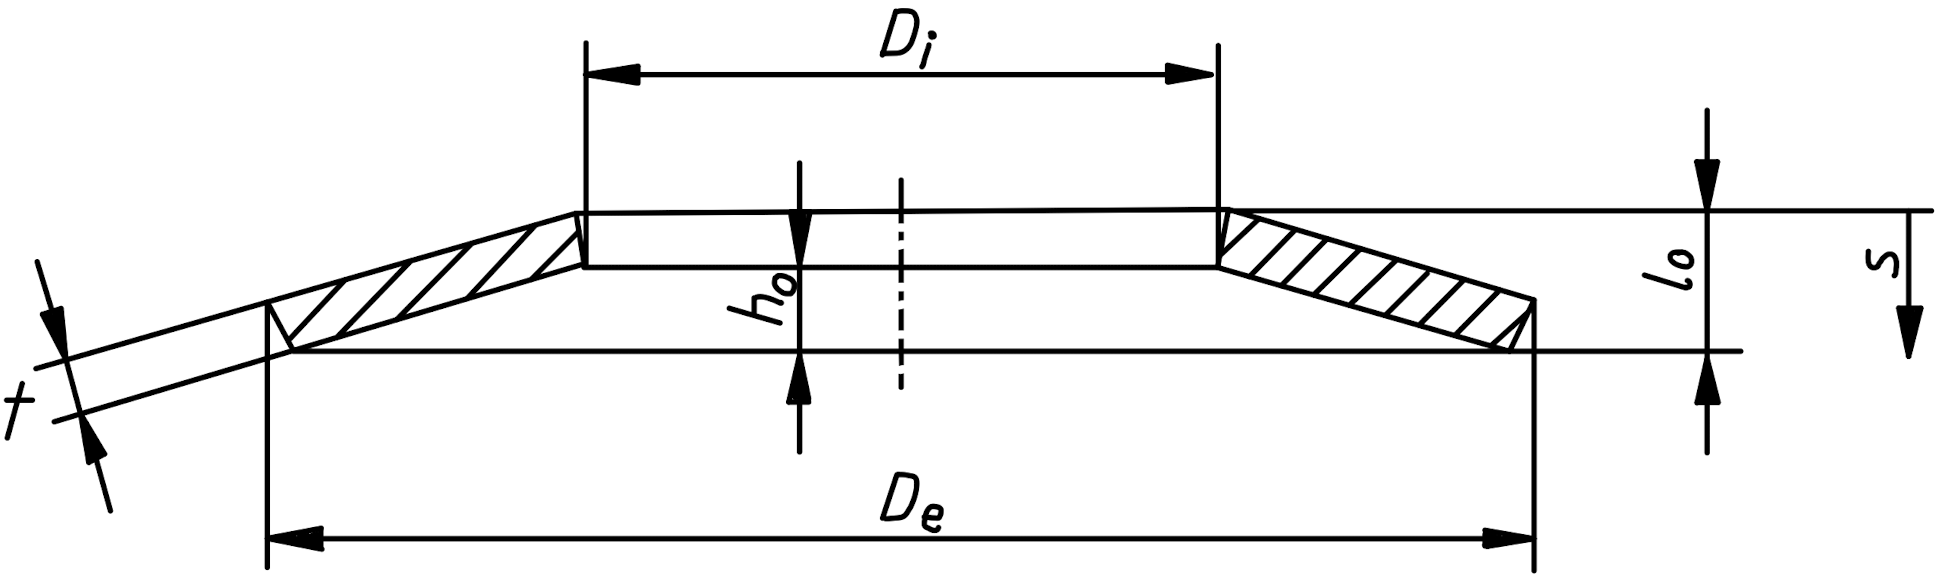
\includegraphics[width = 0.7\linewidth]{src/images/MAEIP_Tellerfeder}
        \begin{minipage}{0.5\linewidth}
            \begin{scriptsize}
                    \begin{tabular}{|c|c|c|}
                    \hline
                    Reihe & $\frac{h_0}{t}$ & Kennlinie\\
                    \hline
                    A & 0.4 & Linear\\
                    \hline
                    B & 0.75 & Mässig degressiv\\
                    \hline
                    C & 1.3 & Stark degressiv\\
                    \hline
                \end{tabular}
            \end{scriptsize}
        \end{minipage}
        \begin{minipage}{0.48\linewidth}
            \vspace{2mm}
            \frame{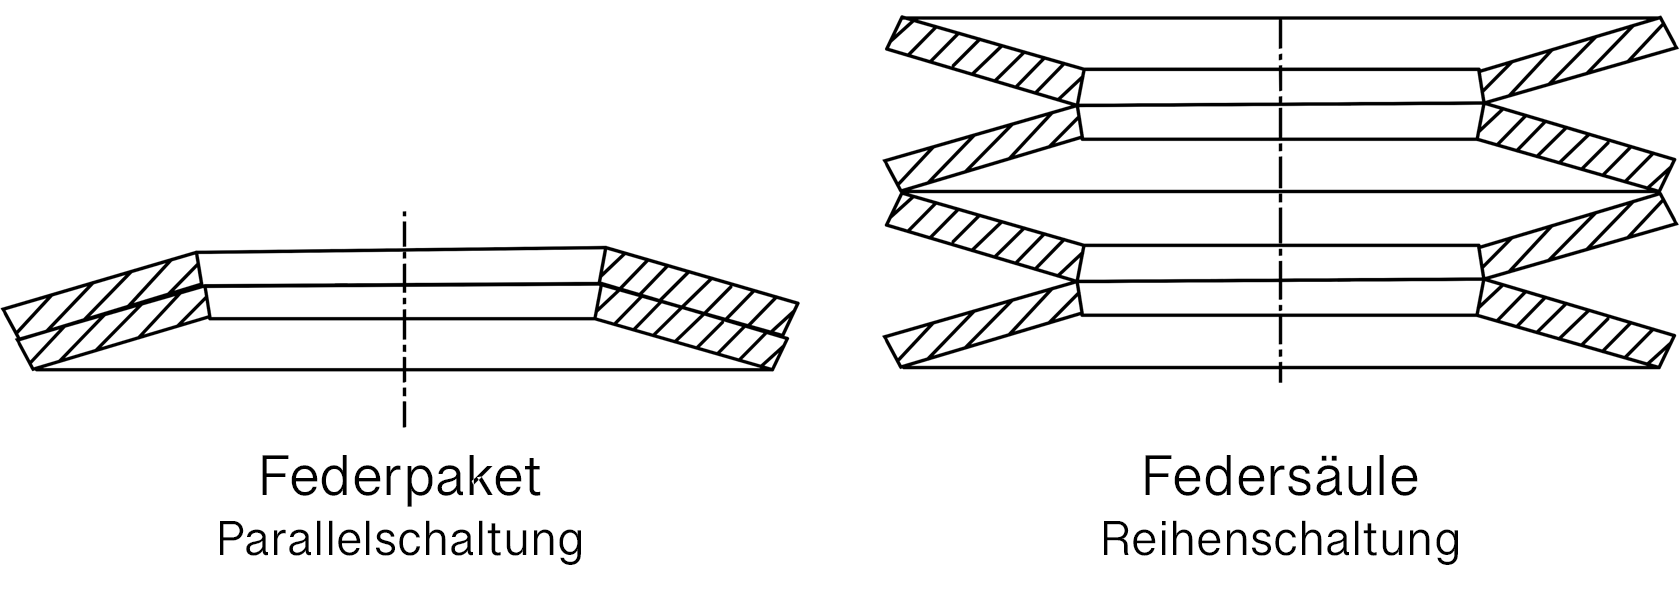
\includegraphics[width = 1.0\linewidth]{src/images/MAEIP_Federpaket}}
        \end{minipage}
        \par \vspace{2mm}
            \begin{scriptsize}
                \textbf{Federsäule:} Reihenschaltung (vgl. 8.2) / \textbf{Federpaket:} Parallelschaltung (vgl. 8.2)
            \end{scriptsize}
    \end{center}
\end{footnotesize}

    \subsection{Drehfedern \hfill ME}
\begin{footnotesize}
    \begin{empheq}[box=\fbox]{align*}
        M = R \cdot \varphi \quad &\mid \quad W = \frac{1}{2} \cdot R\cdot(\varphi_2^2 - \varphi_1^2)
        \\ \tau_{max} = \frac{T}{W_T} \quad &\mid \quad W_T = \frac{\pi R^3}{2}
        \\ \text{Schenkelfeder:} \quad R &= \frac{\pi}{180^\circ} \cdot \frac{E\cdot d^4}{64 \cdot D \cdot n}
        \\ \text{Drehstabfeder:} \quad R &= \frac{\pi}{180^\circ} \cdot \frac{\pi \cdot G \cdot d^4}{32\cdot l_f}
    \end{empheq}
    \begin{scriptsize}
        $M$ = Moment; $\varphi$ = Verdrehwinkel; $W$ = Arbeit; $E$ = E-Modul; $G$ = G-Modul; \\$n$ = Anzahl federnder Windungen; $l_f$ = best. Länge bei Drehstabfeder (idR gegeben) 
    \end{scriptsize}
\end{footnotesize}
    \subsection{Biegefeder \hfill ME}
\vspace*{-1em}
\begin{footnotesize}
    \begin{center}
        \begin{minipage}{0.5\linewidth}
            \mathbox{
                R = \frac{b \cdot h^3 \cdot E}{q_1 \cdot l^3}
            }
        \end{minipage}
        \begin{minipage}{0.48\linewidth}
            \begin{scriptsize}
                \begin{align*}
                    \text{Quadrat:}& \; q_1 = 4
                    \\\text{Dreieck:}& \; q_1 = 6
                    \\\text{Parabel:}& \; q_1 = 8
                    \\~\\ E &= \text{E-Modul}
                \end{align*}
            \end{scriptsize}
        \end{minipage}
    \end{center}
    \scriptsize{\textbf{Zweiarmige Blattfeder:} \\$\to$ Parallelschaltung zweier einarmiger Blattfedern mit $l = \frac{1}{2}$}
\end{footnotesize}
\vspace*{-0.5em}
    \subsection{Schnappverbindung \hfill ME}
\begin{footnotesize}
    \begin{minipage}{0.58\linewidth}
        \begin{center}
            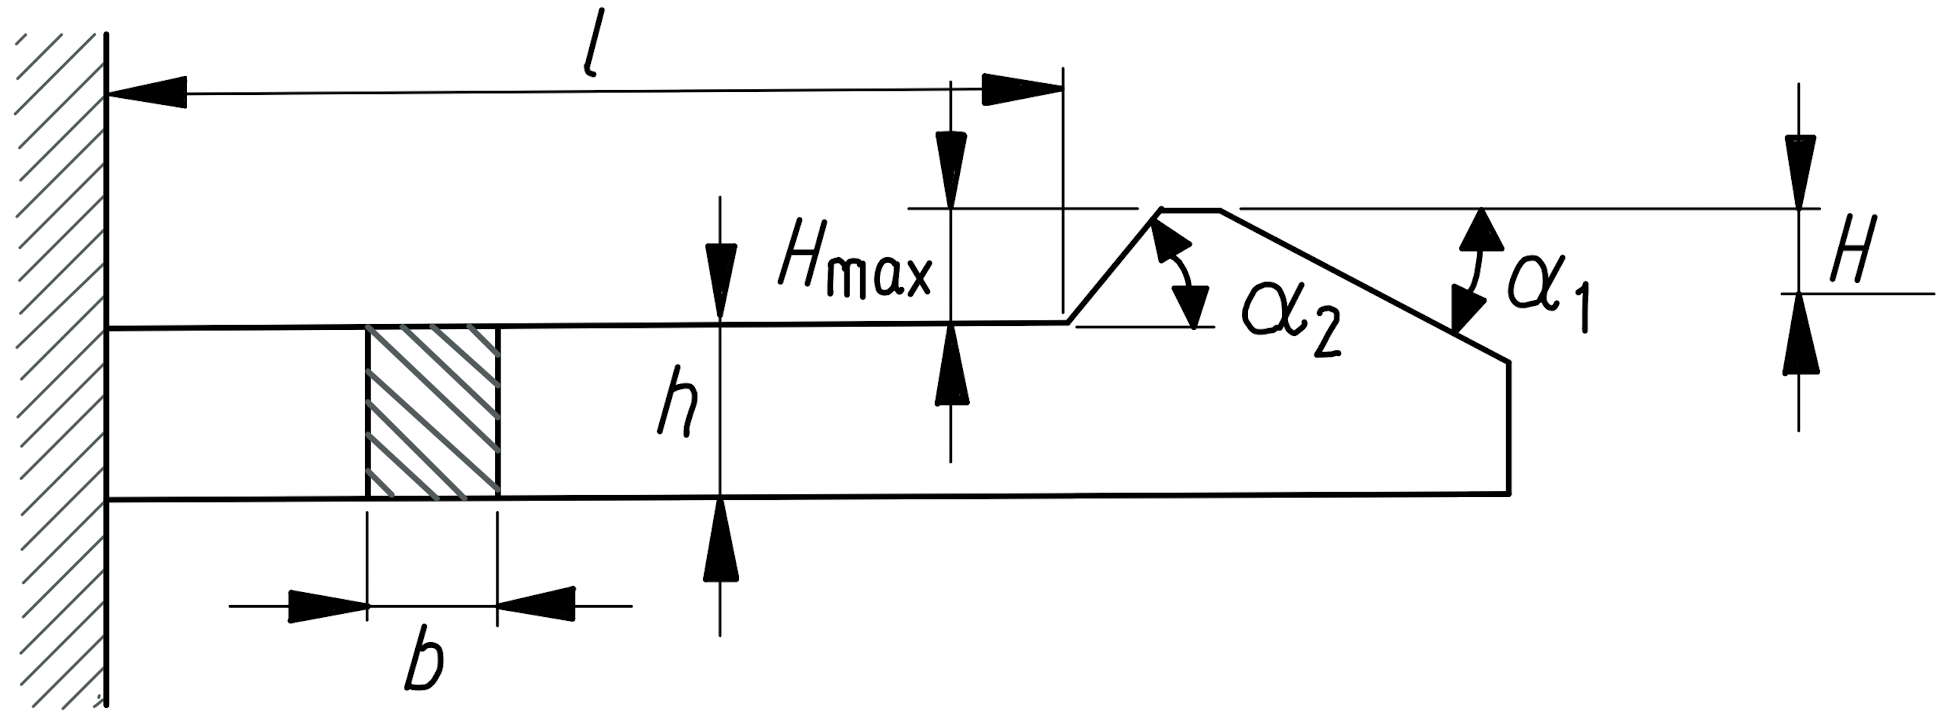
\includegraphics[width = 0.9\linewidth]{src/images/MAEIP_Schnappverbindung}
        \end{center}
    \end{minipage}
    \begin{minipage}{0.4\linewidth}
        \begin{center}
            \begin{empheq}[box=\fbox]{align*}
                s &= H
                \\l_f &= l + \frac{H}{tan(\alpha_2)}
            \end{empheq}
        \end{center}
    \end{minipage}
\end{footnotesize}
    \newpage

\section{Kupplungen \hfill ME}
    \subsection{nicht schaltbar \hfill ME}
    \begin{footnotesize}
        \begin{center}
            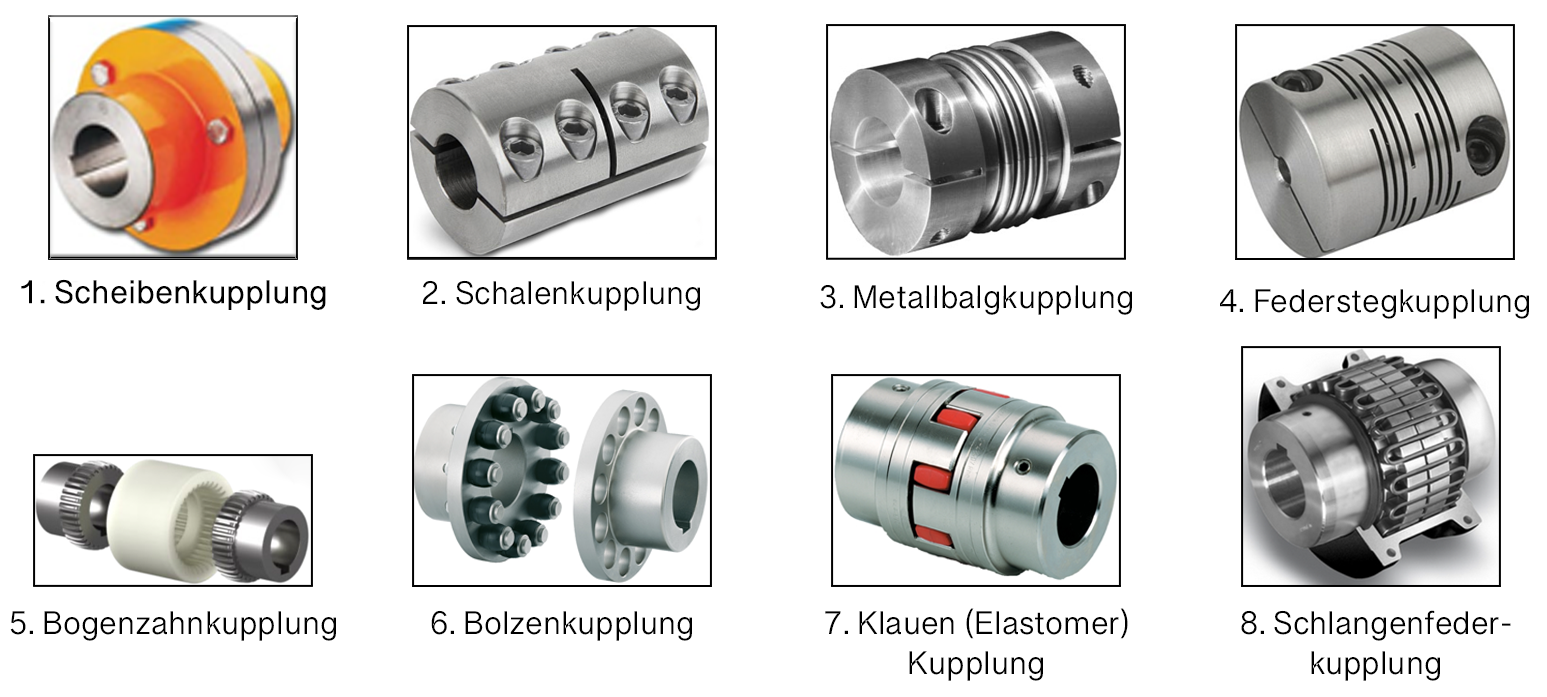
\includegraphics[width = 1.0\linewidth]{src/images/MAEIP_Kupplungen_nichtschaltbar}
                \begin{scriptsize}
                    \begin{tabular}{|c|c|c|c|c|c|c|c|}
                    \hline
                    \multirow{2}{0.01cm}{\null}& \multicolumn{2}{p{1.2cm}|}{\centering Drehnachgieb.} & \multicolumn{2}{p{0.9cm}|}{\centering Drehleist.} & \multicolumn{3}{p{0.9cm}|}{\centering Versatz} \bigstrut \\
                    \cline{2-8} & \multicolumn{1}{c|}{steif} & \multicolumn{1}{c|}{elastisch} & \multicolumn{1}{c|}{Moment} & \multicolumn{1}{c|}{Zahl} & \multicolumn{1}{c|}{Ax.} & \multicolumn{1}{c|}{Rad.} & \multicolumn{1}{c|}{Wink.} \bigstrut \\ \hline
                    1. & X & - & $\uparrow \uparrow / \uparrow\uparrow\uparrow$ & $\downarrow / \to$& none & none & none \bigstrut \\
                    \hline
                    2. & X & - & $\downarrow / \uparrow$ & $\downarrow / \to$ & none & none & none\bigstrut \\
                    \hline
                    3. & X & - & $\to / \uparrow$ & $\to / \uparrow$ & gut & gut & s. gut\bigstrut \\
                    \hline
                    4. & X & - & $\downarrow / \to$ & $\to / \uparrow$ & s. beg. & gut & gut\bigstrut \\
                    \hline
                    5. & X & - & $\uparrow / \uparrow\uparrow$ & $\to / \uparrow$ & gut & s. gut & gut\bigstrut \\
                    \hline
                    6. & - & X & $\uparrow / \uparrow\uparrow$ & $\downarrow / \to$ & gut & s. beg. & gut\bigstrut \\
                    \hline
                    7. & - & X & $\downarrow / \to$ & $\to / \uparrow$ & gut & s. beg. & gut\bigstrut \\
                    \hline
                    8. & - & X & $\to / \uparrow$ & $\downarrow / \to$ & gut & gut & gut\bigstrut \\
                    \hline
                    \end{tabular}
                \end{scriptsize}
        \end{center}
    \end{footnotesize}

    \subsubsection{Kupplungen mit grossem Radialversatz \hfill ME}
        \begin{footnotesize}
            \begin{center}
                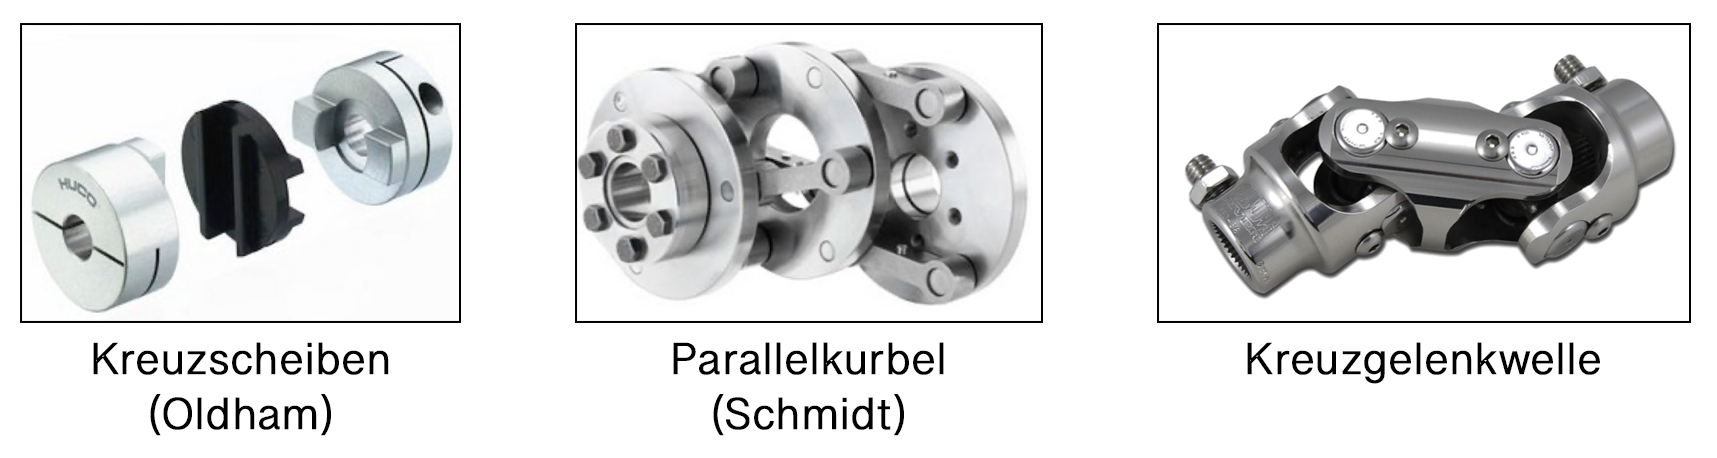
\includegraphics[width = 0.8\linewidth]{src/images/MAEIP_KupplungenRadialversatz}
            \end{center}
        \end{footnotesize}

    \subsection{Schaltbar \hfill ME}
\subsubsection{Fliehkraftkupplung \hfill ME}
\begin{footnotesize}
    \begin{center}
        \scriptsize{\textbf{ohne Abstand zw. Fliehgewicht und Trommel:}}
        \begin{empheq}[box=\fbox]{align*}
            x = \frac{\text{Federn}}{\text{Gewichte}} \mid F_F = F_Z \quad \mid \quad \omega = 2\pi \cdot n
            \\ F_F = F_v \cdot x \quad \mid \quad F_Z = m\cdot r_s \omega^2 \quad \mid \quad \text{\textcolor{Red}{EINHEITEN!}}
            \\ n_G > \sqrt{\frac{F_F}{4 \cdot \pi^2 \cdot m \cdot r_s}} \: [s^{-1}] \xrightarrow{\cdot 60} [min^{-1}]
        \end{empheq}
        \scriptsize{\textbf{mit Auslenkung $a$ des Fliehgewichtes:}}
        \begin{empheq}[box=\fbox]{align*}
            F_F = F_Z \quad \mid \quad \omega = 2\pi \cdot n
            \\F_F = x \cdot(F_v + 2 \cdot R \cdot a) \quad \mid \quad F_Z = m \cdot (r_s + a) \omega^2
            \\n_E > \sqrt{\frac{F_F}{4 \cdot \pi^2 \cdot m \cdot (r_s + a)}} \: [s^{-1}] \xrightarrow{\cdot 60} [min^{-1}]
        \end{empheq}
        \scriptsize{\textbf{Übertragung $M_{\text{max}}$ mit $\mu$ und Auslenkung $a$ des Fliehgewichtes:}}
        \begin{empheq}[box=\fbox]{align*}
            M_{\text{max}} = F_R \cdot r_k = y \cdot \mu \cdot F_N \cdot r_k \quad \mid \quad F_N = \frac{M_{max}}{y \mu r_k}
            \\F_Z = F_N + F_{F} \quad \mid \quad \omega = 2\pi \cdot n
            \\F_F = x \cdot(F_v + 2 \cdot R \cdot a) \quad \mid \quad F_Z = m \cdot (r_s + a) \omega^2
            \\n_B = \sqrt{\frac{F_F + F_N}{4 \cdot \pi^2 \cdot m(r_s + a)}} \: [s^{-1}] \xrightarrow{\cdot 60} [min^{-1}]
        \end{empheq}
        \begin{scriptsize}
            $F_Z = \text{Zentrifugalkraft}; \; F_v = \text{Vorspannkraft}; \; m = \text{Masse Fliehgewicht} [kg];$
            \\ $r_s = \text{Radius Schwerpunkt} [m]; \; R = \text{Federrate pro Feder}; \; n_E = \text{Einschaltdrehzahl};$
            \\ $n_G = \text{Grenzdrehzahl}; \; \mu = \text{Reibwert}; \; x = \text{Anzahl Federn pro Fliehgewicht};$
            \\ $r_k = \text{Innenradius Trommel}; \; a = \text{Abstand zwischen Fliehgewicht und Trommel} [m]$
            \\ $F_F = \text{Federkraft (aller Federn)}; \; y = \text{Anzahl Fliehgewichte}$
        \\~\\ \textcolor{Red}{ACHTUNG: $n_X = [s^{-1}]$}
        \end{scriptsize}
    \end{center}
\end{footnotesize}

\subsubsection{Rutschkupplung \hfill ME}
\begin{footnotesize}
    \begin{center}
        \begin{empheq}[box=\fbox]{align*}
            M_G &= F_t \cdot r_m = F_R \cdot r_m = i \mu_G \cdot F_N \cdot r_m 
            \\&= i \mu_G \cdot F_v \cdot r_m 
            \\r_m &= \frac{d_a + d_i}{4} \quad \mid \quad p = \frac{F_v}{A_m} \quad \mid \quad A_m = \frac{\pi}{4}(d_a^2-d_i^2)
            \\ &\textbf{wenn zusätzlicher Weg $\Delta s$:} 
            \\ F_{v, \text{neu}} &= F_v + R_{\text{ers} \cdot \Delta s} \Rightarrow M_G = i \cdot \mu_G \cdot F_{v, \text{neu}} \cdot r_m
        \end{empheq}
        \begin{scriptsize}
            $M_G = \text{Grenzdrehmoment}; \; F_N = \text{Normalkraft}; \; F_R = \text{Reibkraft}; \;$
            \\$\mu_G = \text{Gleitreibungskoeffizient}; \; r_m = \text{mittlerer Scheibenrand}; \; i = \text{Anzahl Reibkontakte}
        $
        \end{scriptsize}
    \end{center}
\end{footnotesize}

\section{Riemen und Kettentriebe \hfill ME}
    \begin{scriptsize}
    \begin{itemize}
        \item \textbf{Flachriemen:} reibschlüssig;
        \\ $\to$ Vorspannkraft von Lager und Wellen aufgenommen
        \item \textbf{Keilriemen:} grössere Normalkräfte im Reibkontakt
        \\ $\to$ höhere Drehmomente
        \item \textbf{Zahnriemen:} kein Schlupf $\to$ Übetragung synchron
        \item \textbf{Kettentrieb:} Übertragung formschlüssig $\to$ synchron / höhere \\ Drehmomente / extremere Temperaturbereiche
        \\\underline{Polygoneffekt:} kein sauberes Abrollen der einzelnen Kettenglieder \\$\to$ Vieleck, Polygon $\to$ Geschwindigkeitsschwankungen
    \end{itemize}
    \begin{empheq}[box=\fbox]{align*}
        &\text{Kettenraddurchmesser}: \quad d_{\text{min}} = d_{\text{max}} \cdot cos\left(\frac{\tau}{2}\right) [m]
        \\ &\text{Kettengeschwindigkeit:} \quad v_{\text{min}} = v_{\text{max}} \cdot cos \left(\frac{\tau}{2}\right) [m/s] 
    \end{empheq}
\end{scriptsize}


\section{Passungen \hfill ME}
    \begin{footnotesize}
    \colorbox{Apricot}{Bohrung: Grossbuchstaben} \hfill \colorbox{SkyBlue}{Welle: Kleinbuchstabe}
    \begin{itemize}
        \item \textbf{Oberes Abmass} (B: ES / W: es) ist immer \textbf{grösser als unteres Abmass} (B: EI / W: ei)
        \item \textbf{Einheitsbohrung: H} Feld für Bohrung
        \item \textbf{Einheitswelle: h} Feld für Welle
        \item \textbf{H/h-Passungen:} immer Spielpassungen
    \end{itemize} 
    \begin{empheq}[box=\fbox]{align*}
        \text{oberes Abmass} &= \text{unteres Abmass} + \text{Toleranzfeldbreite}
        \\\text{unteres Abmass} &= \text{oberes Abmass} - \text{Toleranzfeldbreite}
        \\S_{\text{min}} &= \text{u.A. (Bohrung)} - \text{o.A. (Welle)}
        \\U_{\text{min}} &= \text{u.A. (Welle)} - \text{o.A. (Bohrung)}
        \\U_{\text{min}} &> 0 \Leftrightarrow \text{immer Übermass}
        \\U_{\text{min}} &< 0 \Leftrightarrow \text{nicht immer Übermass}
        \\S_{\text{min}} &> 0 \Leftrightarrow \text{immer Spiel}
        \\S_{\text{min}} &< 0 \Leftrightarrow \text{nicht immer Spiel}
    \end{empheq}
\end{footnotesize}
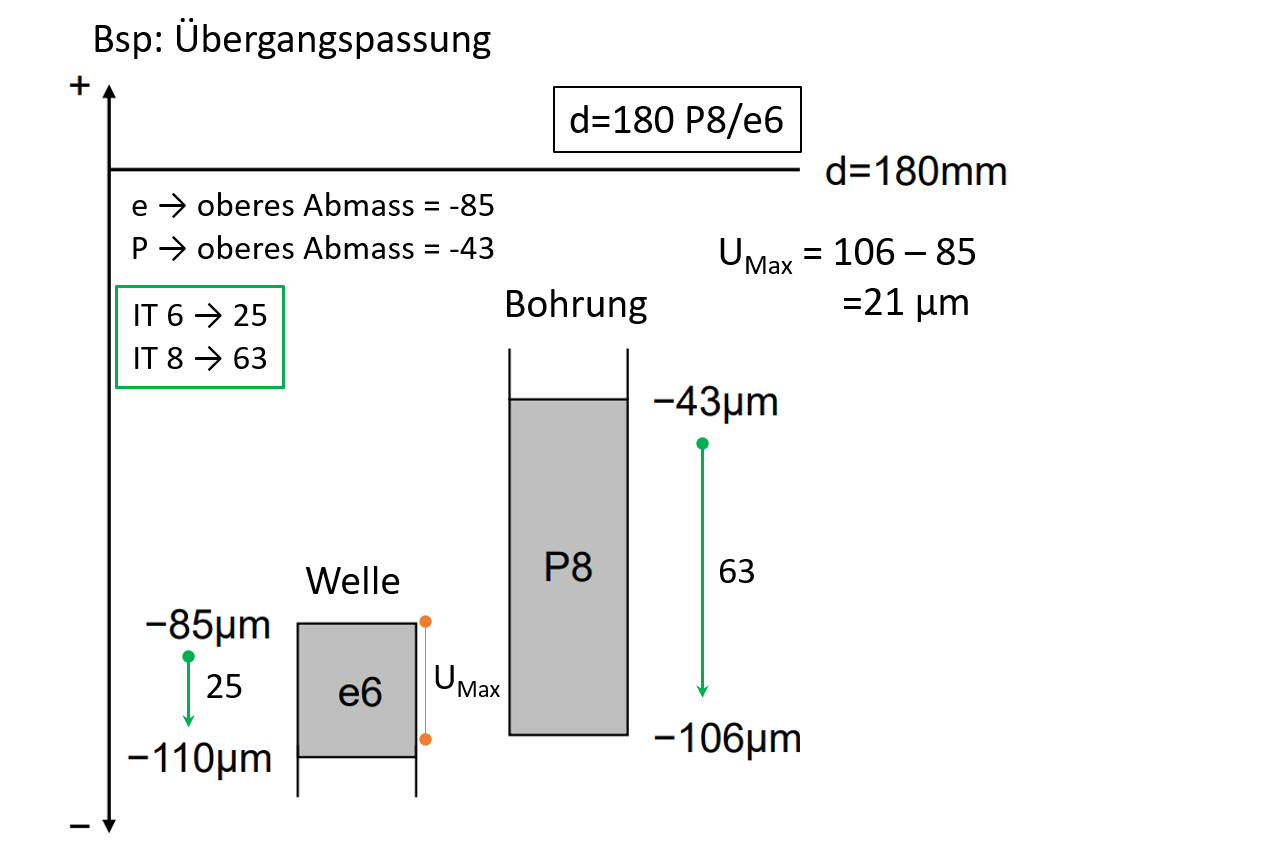
\includegraphics[width = 0.9\linewidth]{src/images/Passungen_bsp.png}


\section{Dichtungen \hfill ME}
    \begin{scriptsize}
    \begin{itemize}
        \item \textbf{Flachdichtungen:} statische Dichtung $\to$ berührend
        \item \textbf{O-Ring:} statische und dynamische Dichtung $\to$ berührend
        \item \textbf{Spaltdichtung:} Fett, trockene und staubfreie Umgebung
        \item \textbf{Labyrinth:} Fett, gut gegen Eindringen von Schmutz
        \item \textbf{Filzring:} Anpassung an Laufgenauigkeit $\to$ günstig
        \item \textbf{V-Ring:} Drehzahl begrenzt $\to$ Öl und Fett
    \end{itemize}
\end{scriptsize}
    \newpage

% \section{Iterativer Ansatz und Methoden \hfill IP}
%     \subsection{Iterativer Ansatz \hfill IP}
\begin{center}
    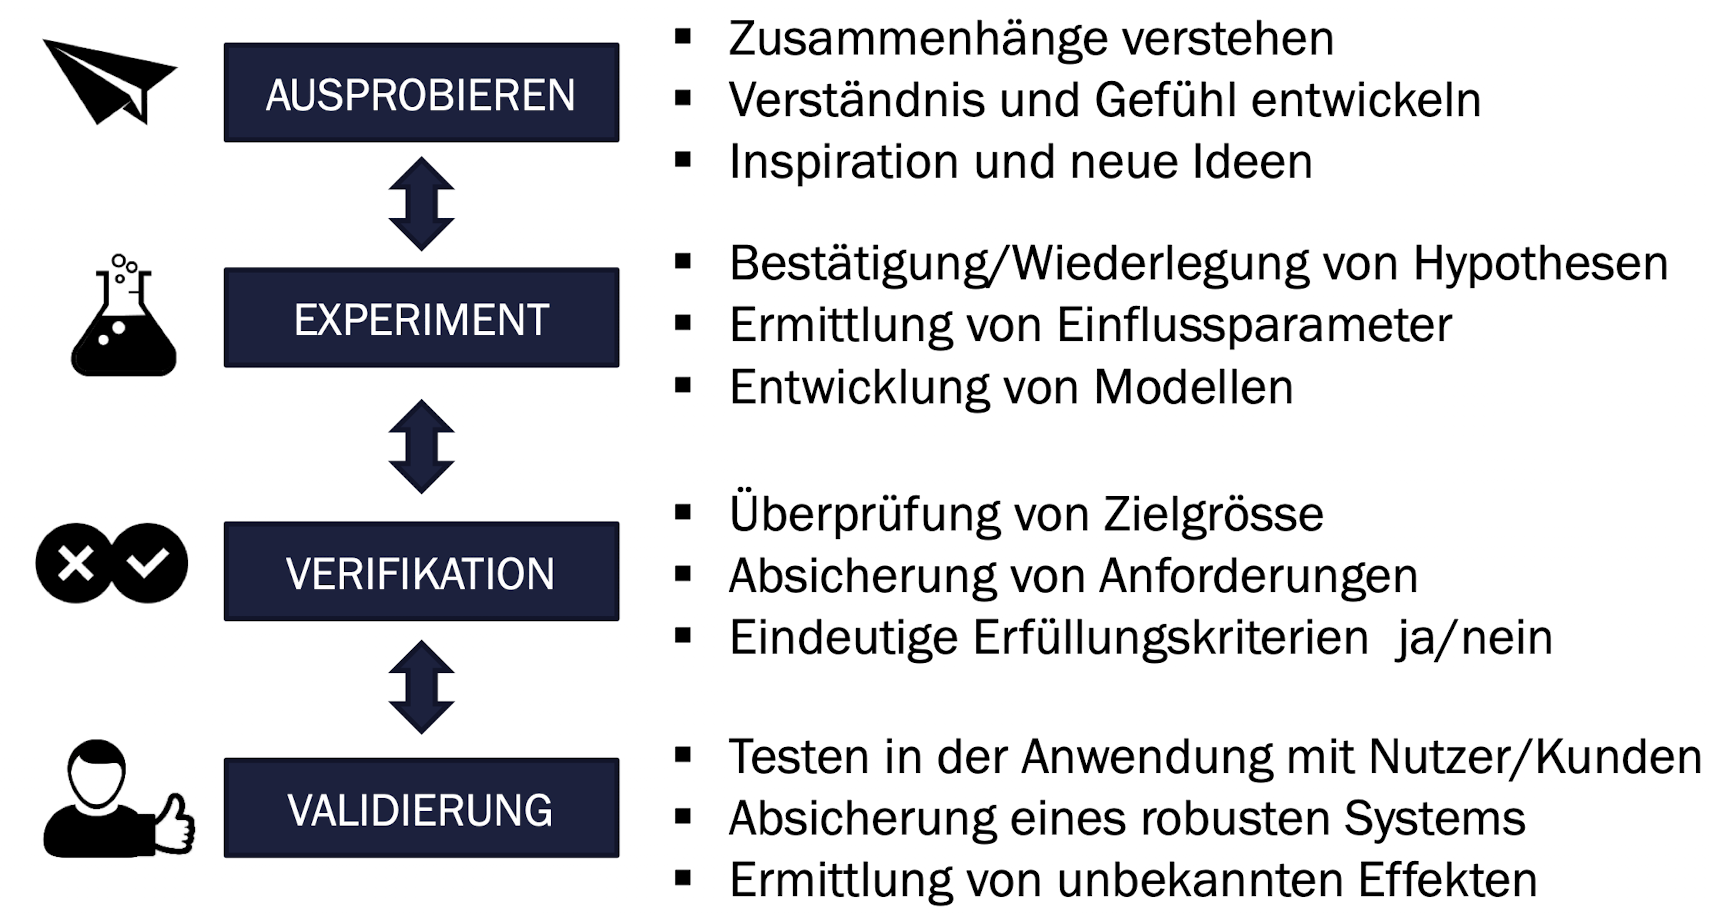
\includegraphics[width = 0.9\linewidth]{src/images/MAEIP_Testing}
\end{center}
%     \subsection{System und Funktion \hfill IP}
\begin{scriptsize}
    \begin{itemize}
        \item \textbf{System:} führt bestimmte Funktionen aus
        \item \textbf{Funktion:} neutrale Beschreibung zwischen Input und Output
        \subitem \textbf{kritische Funktion:} oft Nebenfunktionen
        \item \textbf{Gesamtfunktion:} erfasst Aufgaben insgesamt
        \item \textbf{Hauptfunktion:} Teilfunktion, die unmittelbar der Gesamtfunktion \\dient
        \item \textbf{Teilfunktion:} Element der Gesamtfunktion
        \item \textbf{Nebenfunktion:} Teilfunktion, die der Gesamtfunktion nur mittelbar \\dient 
    \end{itemize}
\end{scriptsize}
%     \subsection{Systemkonzepte nach Ropohl \hfill IP}
\begin{footnotesize}
    \begin{center}
        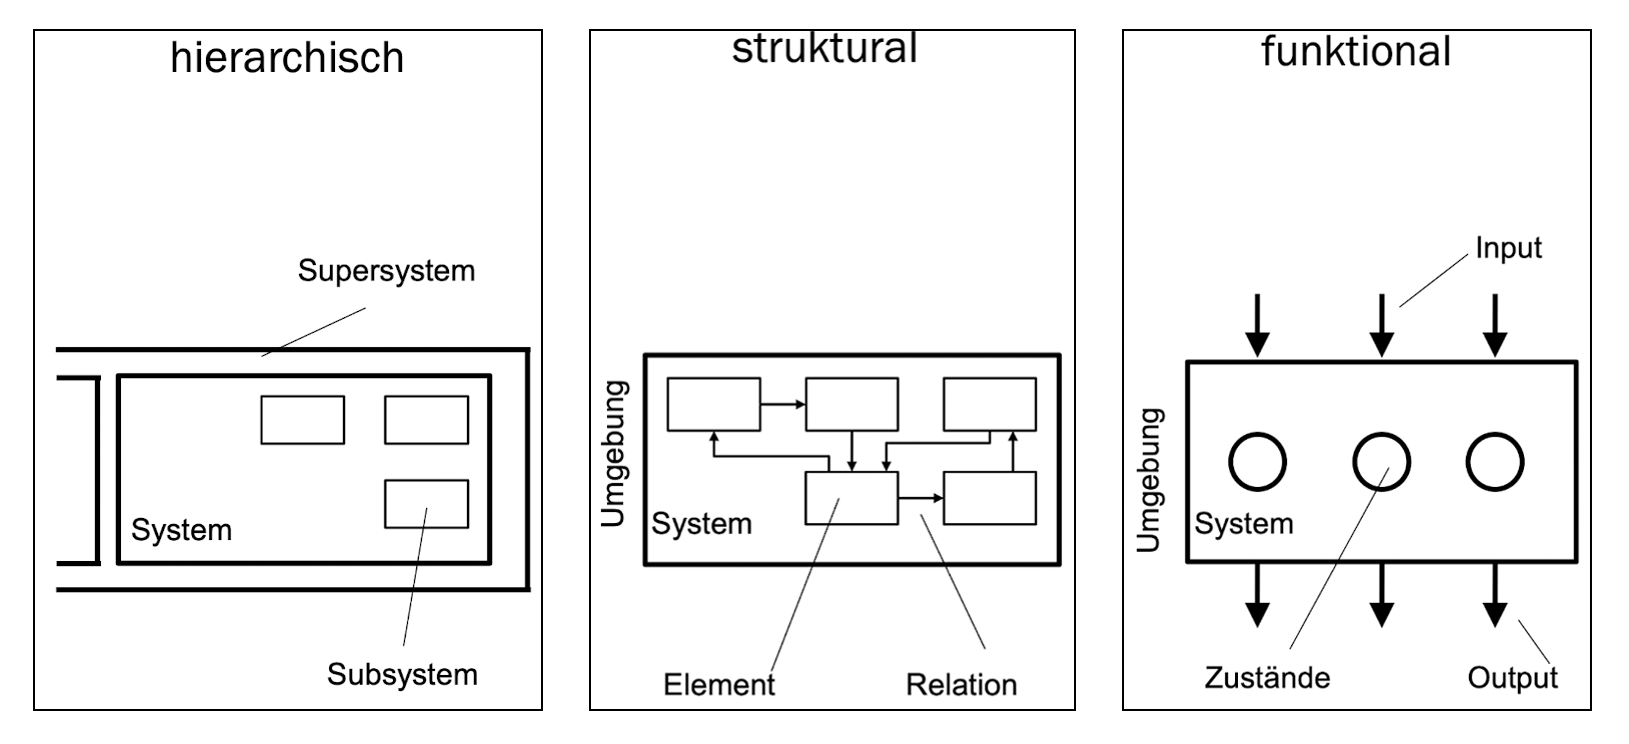
\includegraphics[width = 1.0\linewidth]{src/images/MAEIP_Ropohl}
    \end{center}
\end{footnotesize}
%     \subsection{Typen von Anforderungen \hfill IP}
\begin{scriptsize}
    \begin{center}
        \begin{tabular}{|c|c|c|c|c|}
            \hline
            Bez. & Typ & Beschreibung & Grössenord. & Bsp. \\
            \hline
            \cellcolor{Apricot} F & Festforderung & \thead{\scriptsize{muss} \\ \scriptsize{erfüllt werden}} & 220V 50Hz & \thead{\scriptsize{Energie} \\\scriptsize{für Ladegerät}}\\
            \hline
            \cellcolor{Melon} B & Bereichsforderung & - & - & - \\
            \hline
            \cellcolor{Melon} B& Intervallforderung & \thead{\scriptsize{Obere und} \\ \scriptsize{untere Schranke}} & $\scriptstyle{2<x<3}$ mm & Sägeblattdicke\\
            \hline
            \cellcolor{Melon} B& Maximalforderung & obere Schranke & $\scriptstyle{< 3.5}$ kg mm & Gewicht\\
            \hline
            \cellcolor{Melon} B& Minimalforderung & untere Schranke & $>1$h & Akkulaufzeit\\
            \hline 
            \cellcolor{Goldenrod} W & Wunschforderung & \thead{\scriptsize{Erfüllung} \\ \scriptsize{ist aufwertend} \\ \scriptsize{Nicht-Erfüllung} \\ \scriptsize{ist kein} \\ \scriptsize{Ausschluss-Kriterium}} & - & \thead{\scriptsize{Autom.} \\ \scriptsize{Ein/Aus}}\\
            \hline
        \end{tabular}
    \end{center}
\end{scriptsize}
%     \subsection{Finden von Lösungen \hfill IP}
    \textbf{Divergenz und Konvergenz}
    \begin{scriptsize}
        \begin{itemize}
            \item \textbf{Divergenz:} Vielfalt von alternativen Lösungsmöglichkeiten erzeugen \\$\to$ Bewusst \underline{keine Bewertung / Auswahl}
            \item \textbf{Konvergenz:} Bewuss \underline{keine neuen Ideen generiern} \\$\to$ Lösungen verlgeichen, eine wählen
        \end{itemize}
    \end{scriptsize}

    \textbf{Vorhandene Lösungen}
    \begin{scriptsize}
        \begin{itemize}
            \item \textbf{Methoden:} Recherche / Lösungskatalog / Physikalische Effekte
            \item \textbf{virtuelle Produkte:} Konstruktionskataloge / Physikalische Effekte / \\Patente
            \item \textbf{Reale Produkte:} Eigene Produkte / Zulieferer / Wettbewerber
        \end{itemize}
    \end{scriptsize}

    \textbf{Intuitive Lösungen}\\
    \begin{scriptsize}
        Brainstorming / Galerie-Methode / Analogiebildung / Mindmapping / 6-3-5-Methode
    \end{scriptsize}
%     \subsection{Variation und Kombination \hfill IP}
\begin{scriptsize}
    \begin{center}
        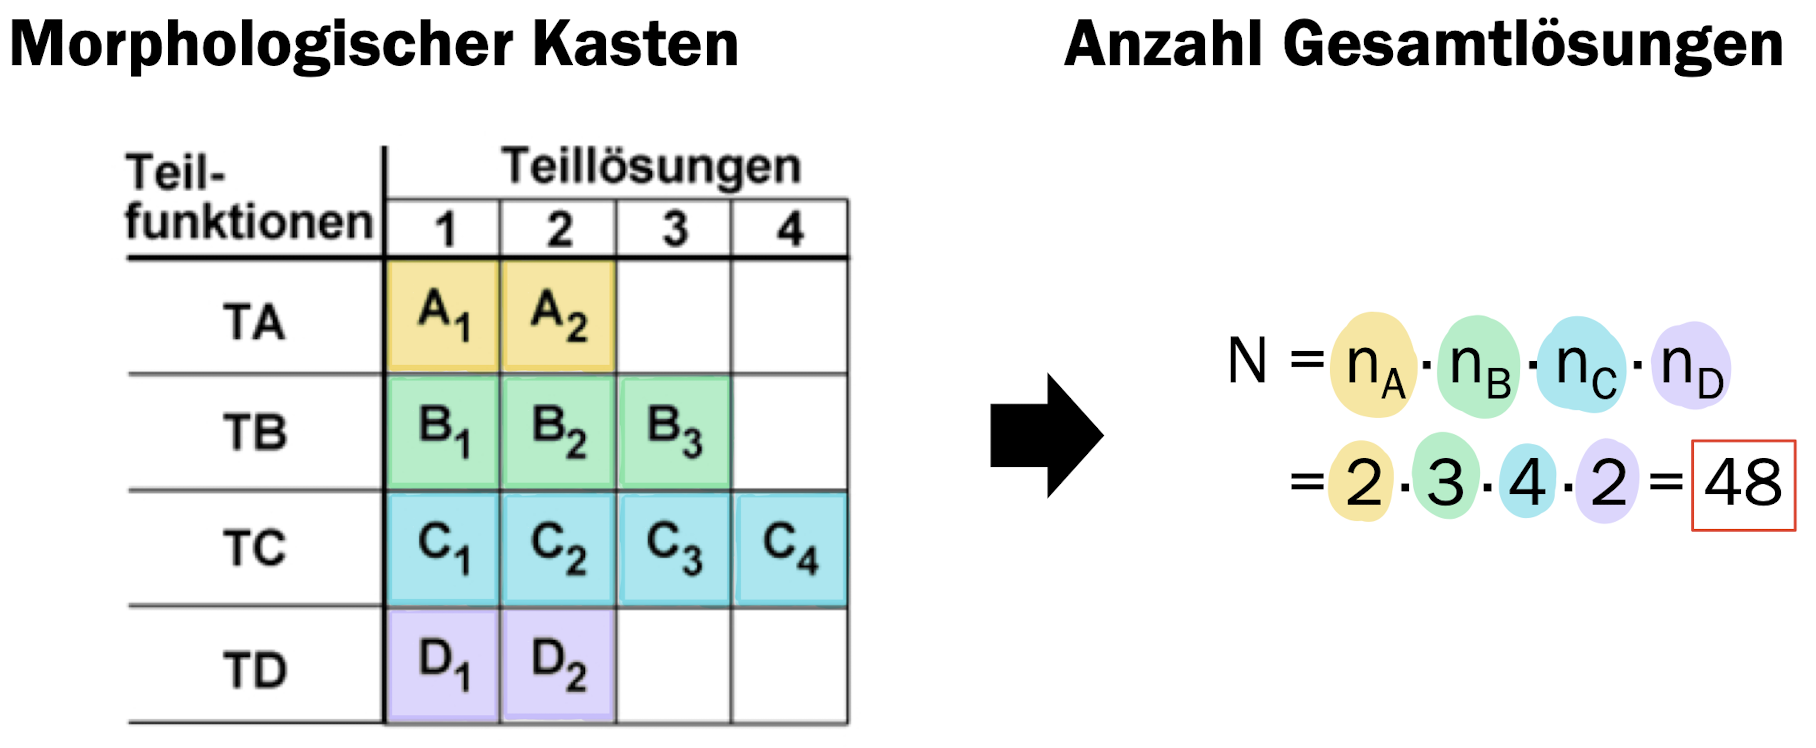
\includegraphics[width = 0.8\linewidth]{src/images/MAEIP_MorphologischerKasten}
    \end{center}
    \begin{empheq}[box=\fbox]{align*}
        &\textbf{Wenn \# unverträglicher} \: \textbf{Kombinationen = 1:} 
        \\ &n_{\text{unverträglich}} = \frac{N_{\text{max}}}{(n_x \cdot n_y)}
        \\ &n_x \& n_y := \text{Anzahl Teillösungen der betroffenen Teilfunktionen}
        \\ & \textbf{Wenn \# unverträglicher Kombinationen $>$ 1: } 
        \\ &\text{Variantenbaum aufstellen}
    \end{empheq}
\end{scriptsize}
%     \subsection{Wirtschaftlich-technischer Vergleich \hfill IP}
\begin{footnotesize}
        \mathbox{
            \textbf{Technischer Vergleich: } \qquad W_t = \frac{\text{Produktleistung}}{\text{Kundenwunsch}}
        }
        \vspace{-2mm}
        \mathbox{
            \textbf{Wirtschaftlicher Vergleich: } \qquad W_w = \frac{\text{Aufwand ideal}}{\text{Aufwand real}}
        }
\end{footnotesize}
%     \subsection{Binärer Vergleich \hfill IP}
\begin{scriptsize}
    \begin{itemize}
        \item Erstelle Tabelle mit Kriterien als Zeilen \textbf{und} Spalten
        \item Vergleiche Spalten und Zeilen folgendermassen:
        \subitem [2]: Spalte ist wichtiger als Zeile 
        \subitem [1]: Spalte und Zeile sind gleichwertig
        \subitem [0]: Spalte ist weniger wichtig als Zeile
        \item Spaltenwerte aufsummieren $\to$ normieren $\to$ prozentuale Wichtigkeit berechnen
    \end{itemize}
\end{scriptsize}
%     \subsection{Nutzwertanalyse [NWA] \hfill IP}
\begin{scriptsize}
    \begin{enumerate}
        \item Bewertungskriterien aus Kundenanforderungen ableiten
        \item Bewertungskriterien gewichten (Binärer Vergleich)
        \item Eigenschaften der Lösungen zusammenstellen
        \item Werteskala auswählen / erarbeiten
        \item Lösungseigenschaften beurteilen
        \item Gesamtwert bilden
    \end{enumerate}
\end{scriptsize}

\section{Mechanische Mechanismen \hfill IP}
    \subsection{Hebel \hfill IP}
\begin{footnotesize}
    \begin{center}
        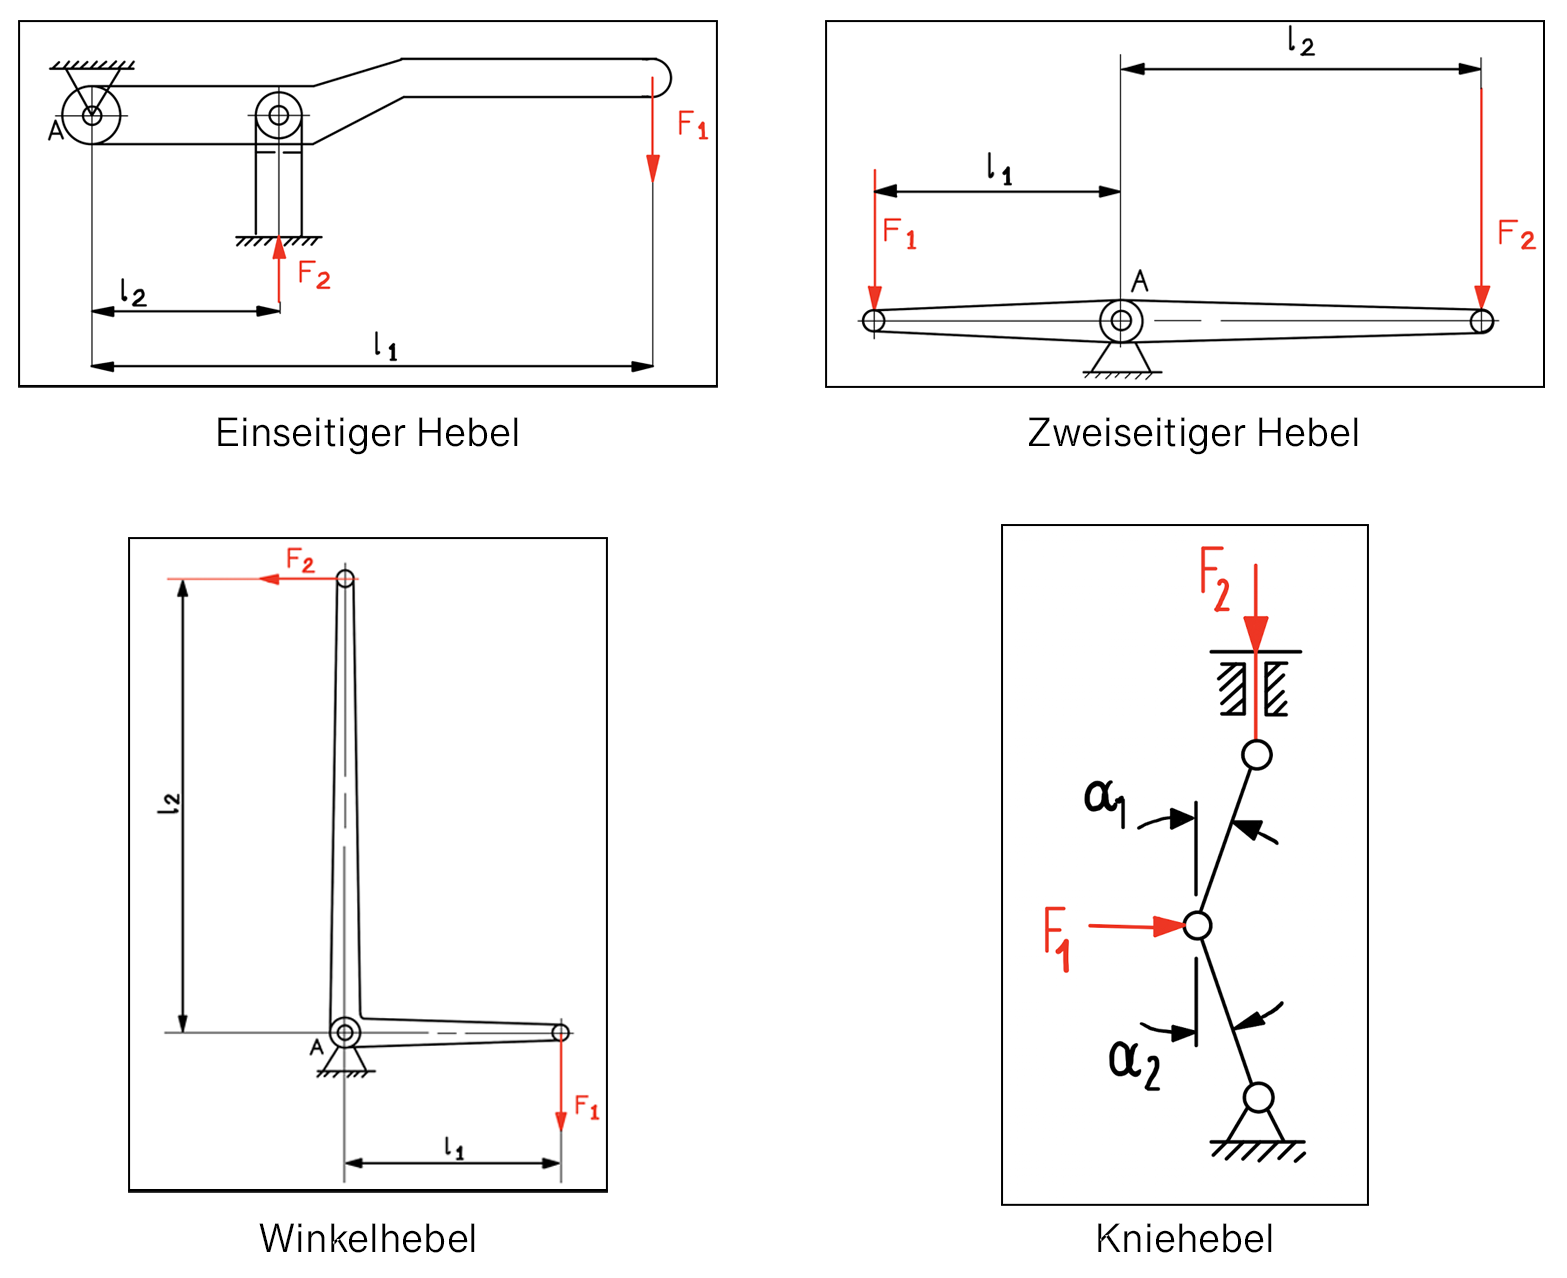
\includegraphics[width = 0.8\linewidth]{src/images/MAEIP_Hebel}
        \includegraphics[width = 0.5\linewidth]{src/images/MAEIP_Serienhebel}
    \end{center}

    \begin{empheq}[box=\fbox]{align*}
        \textbf{Allgemein: }F_2 &= \frac{l_1}{l_2}\cdot F_1
        \\\textbf{Kniehebel: }F_2 &= \frac{F_1}{tan(\alpha_1) + tan(\alpha_2)} 
        \\\textbf{Serienschaltung: }F_3 &= \frac{l_1}{l_2} \cdot \frac{l_3}{l_4} \cdot F_1
    \end{empheq}
\end{footnotesize}
    \subsection{Schiefe Ebene \hfill IP}
\begin{footnotesize}
    \begin{center}
        \begin{minipage}{0.4\linewidth}
        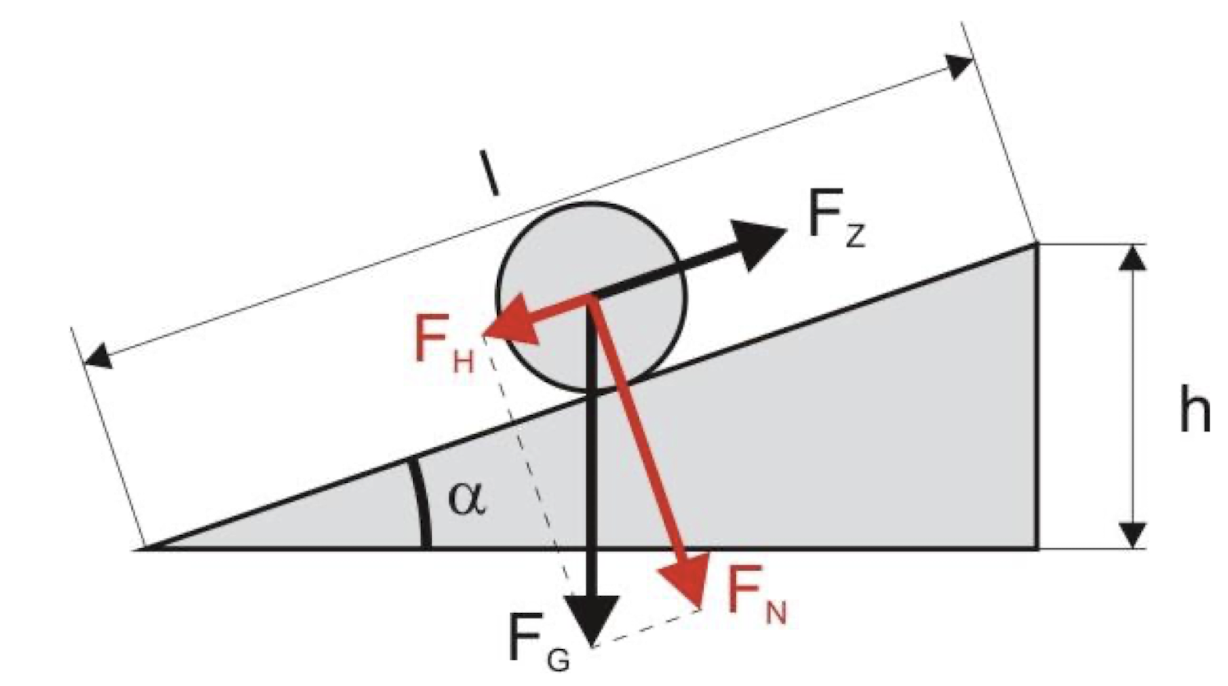
\includegraphics[width = 1.0\linewidth]{src/images/MAEIP_SchiefeEbene}
        \end{minipage}
        \begin{minipage}{0.58\linewidth}
            \begin{empheq}[box=\fbox]{align*}
                F_G &= \frac{l}{h} \cdot F_Z
                \\ &= \frac{1}{sin(\alpha)} \cdot F_Z
            \end{empheq}
        \end{minipage}
    \end{center}
\end{footnotesize}
    \subsection{Keil \hfill IP}
\begin{footnotesize}
    \begin{center}
        \begin{minipage}{0.4\linewidth}
            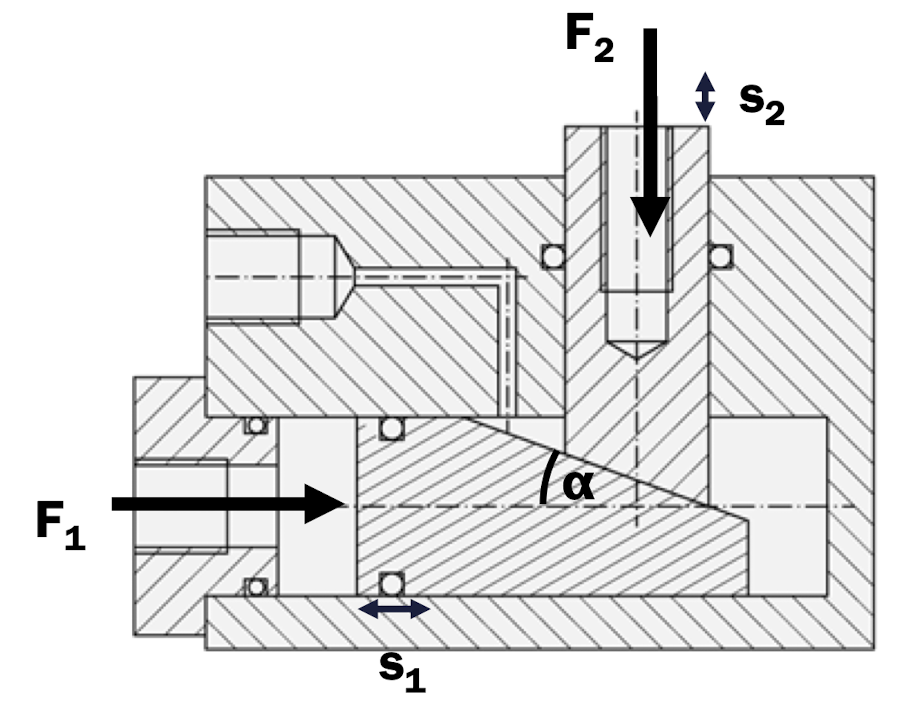
\includegraphics[width = 0.9\linewidth]{src/images/MAEIP_Keil}
        \end{minipage}
        \begin{minipage}{0.58\linewidth}
            \begin{empheq}[box=\fbox]{align*}
                F_2 &= \frac{s_1}{s_2} \cdot F_1
                \\F_2 &= \frac{1}{tan(\alpha)} \cdot F_1
            \end{empheq}
        \end{minipage}
    \end{center}
\end{footnotesize}
    \subsection{Schraube \hfill IP}
\begin{footnotesize}
    \begin{center}
        \begin{minipage}{0.52\linewidth}
            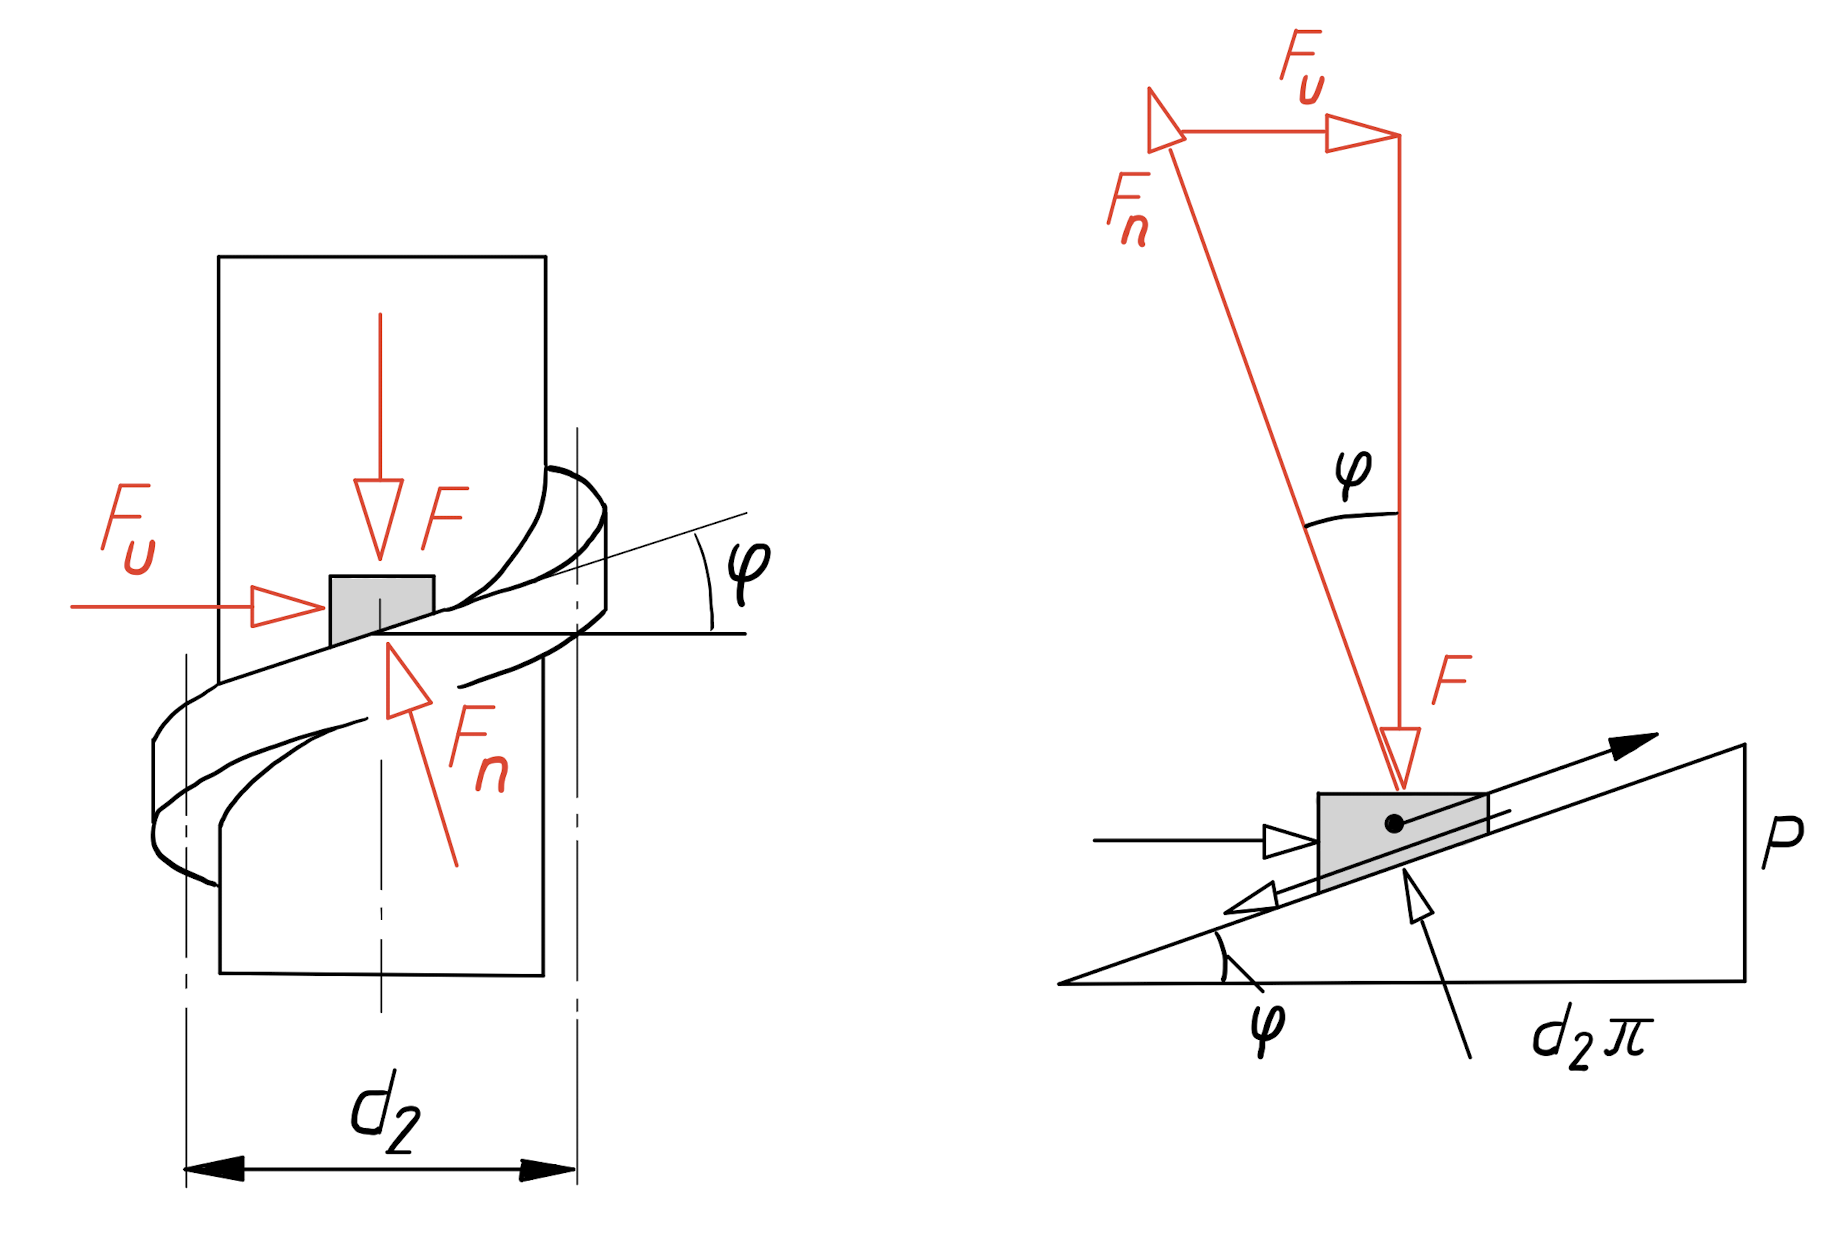
\includegraphics[width = 0.9\linewidth]{src/images/MAEIP_SchraubeIP}
        \end{minipage}
        \begin{minipage}{0.46\linewidth}
            \begin{empheq}[box=\fbox]{align*}
                F = \frac{1}{tan(\phi)} \cdot F_U
            \end{empheq}
        \end{minipage}
    \end{center}
\end{footnotesize}
    \cbreak
    \subsection{Seilzug \hfill IP}
\begin{footnotesize}
    \begin{center}
        \begin{minipage}{0.58\linewidth}
            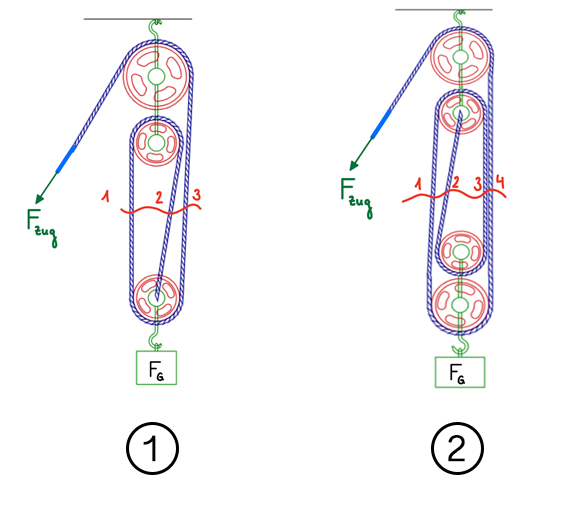
\includegraphics[width = 1.0\linewidth]{src/images/MAEIP_Seilzug1}
            \\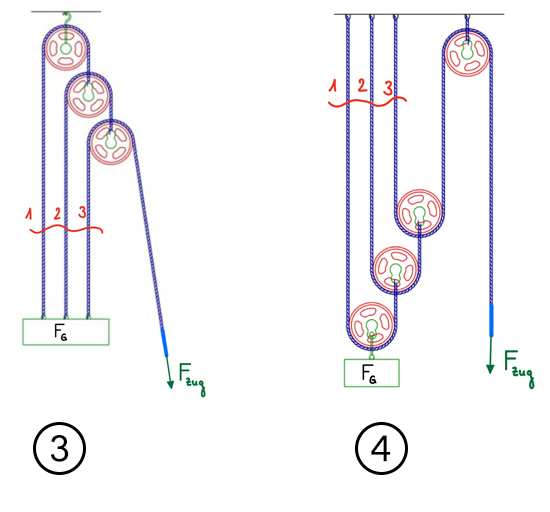
\includegraphics[width = 0.9\linewidth]{src/images/MAEIP_Seilzug2}
        \end{minipage}
        \begin{minipage}{0.4\linewidth}
            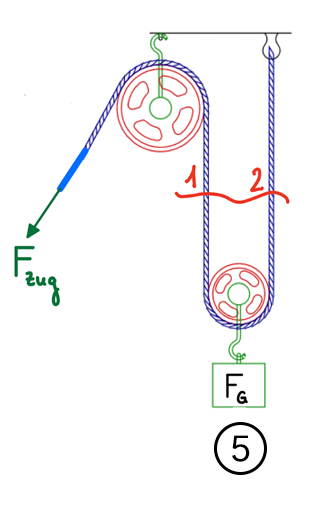
\includegraphics[width = 0.7\linewidth]{src/images/MAEIP_Seilzug3}
            \begin{empheq}{align*}
                1. \; \; F_{\text{zug}} &= \frac{1}{3} \cdot F_G 
                \\ 2. \; \; F_{\text{zug}} &= \frac{1}{4} \cdot F_G 
                \\ &= \frac{1}{n} \cdot F_G
                \\ 3. \; \; F_{\text{zug}} &= \frac{1}{7} \cdot F_G 
                \\ 4. \; \; F_{\text{zug}} &= \frac{1}{8} \cdot F_G 
                \\ &= \frac{1}{2^3} \cdot F_G
                \\ 5. \; \; F_{\text{zug}} &= \frac{1}{2} \cdot F_G
            \end{empheq}
        \end{minipage}
    \end{center}
    \begin{empheq}[box=\fbox]{align*}
        \textbf{Wirkungsgrad:  } \eta_F = \eta_R^{\text{\# Rollen}} \quad \mid \quad F_z = \frac{F_g}{\text{\# Rollen}} \cdot \frac{1}{\eta_F}
    \end{empheq}
\end{footnotesize}
    \subsection{Schubkurbel \hfill IP}
\begin{footnotesize}
    \begin{center}
        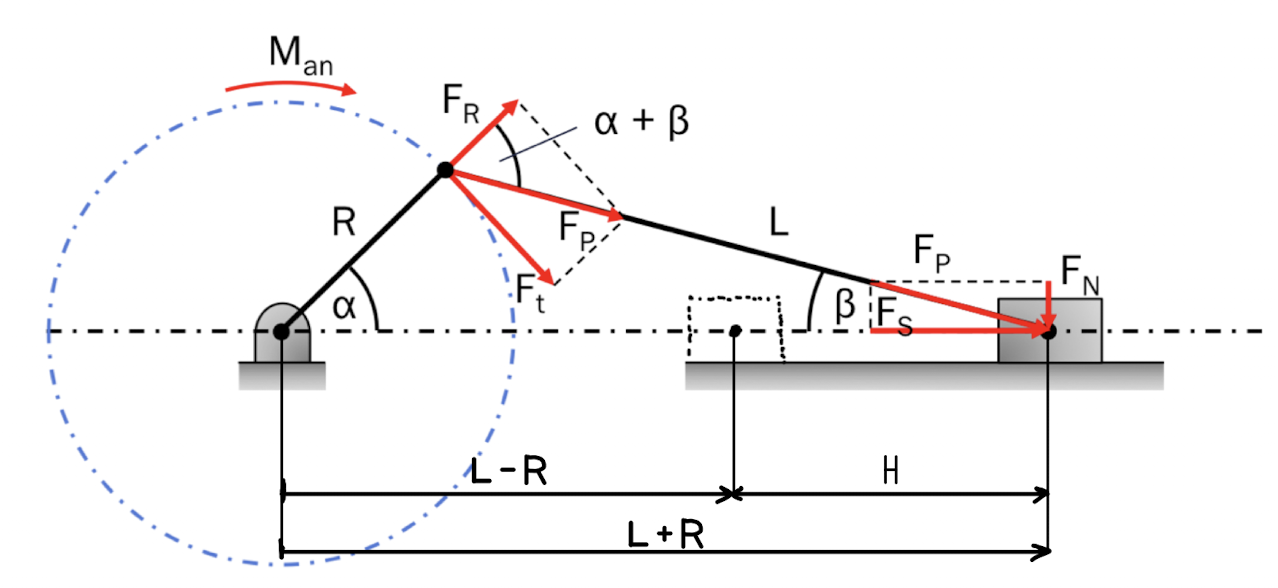
\includegraphics[width = 0.8\linewidth]{src/images/MAEIP_Schubkurbel}
        \begin{empheq}[box=\fbox]{align*}
            H = 2\cdot R \quad \mid \quad t = &\frac{1}{n} \quad \mid \quad \lambda = \frac{R}{L} = \frac{sin(\beta)}{sin(\alpha)}
            \\F_s = \frac{cos(\beta) \cdot M_{an}}{sin(\alpha + \beta) \cdot R} \quad &\mid \quad sin(\alpha + \beta) = \frac{F_t}{F_p}
            \\F_t = \frac{M_{an}}{R} \quad &\mid \quad cos(\beta) = \frac{F_s}{F_p}
        \end{empheq}
        $H$ = Hublänge; $t$ = Taktzeit (1x Hin und zurück); \\$\lambda$ = Schubstangenverhältnis (meist $0.1 \leq \lambda \leq 0.4$); $n$ = Drehzahl
    \end{center}
\end{footnotesize}

\subsubsection{Variation Kurbellänge \hfill IP}
\begin{footnotesize}
    \begin{center}
        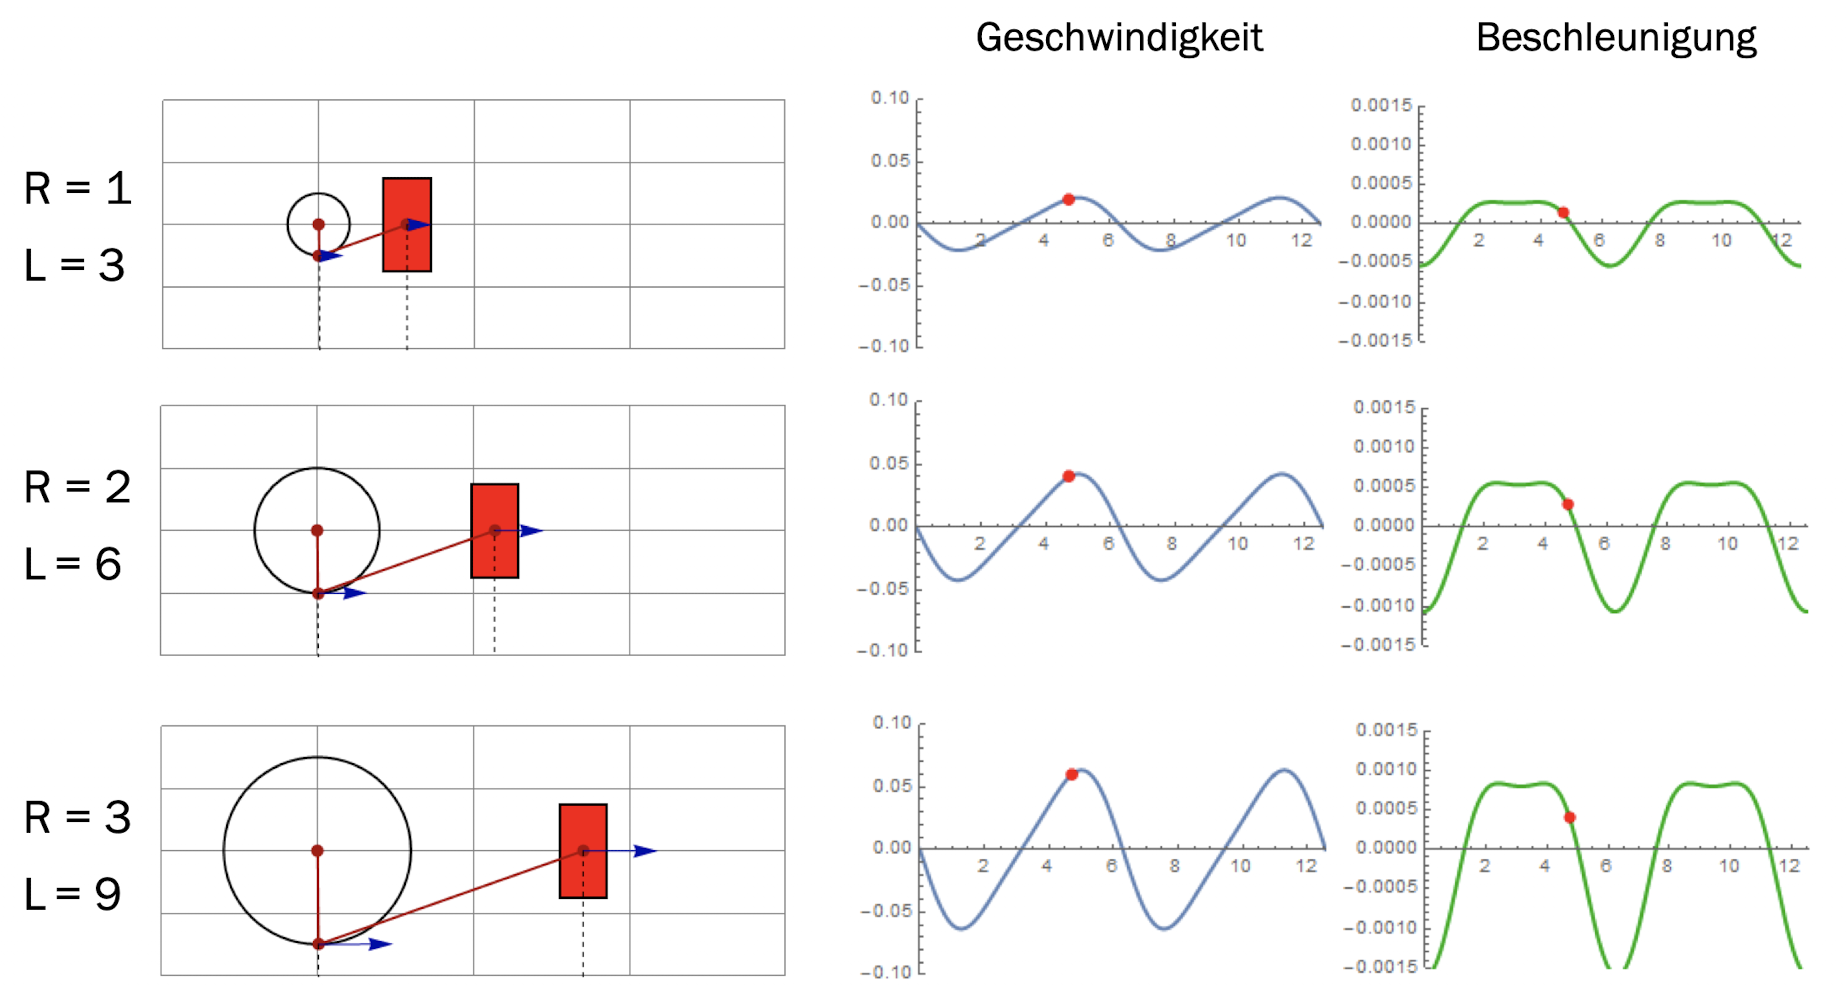
\includegraphics[width = 0.8\linewidth]{src/images/MAEIP_VariationKurbellaenge}
    \end{center}
    \begin{itemize}
        \item \textbf{Kurze Kurbel} $\to$ kleine Amplitude 
        \item \textbf{Lange Kurbel} $\to$ grosse Amplitude
        \item \textbf{Grosses Schubstangenverhältnis [R/L]} $\to$ Schwingung mit Senke
        \item \textbf{Kleines Schubstangenverhältnis [R/L]} $\to$ Schwingung ohne Senke
    \end{itemize}
\end{footnotesize}

\subsubsection{Variation Pleuellänge \hfill IP}
\begin{footnotesize}
    \begin{center}
        \includegraphics[width = 0.8\linewidth]{src/images/MAEIP_VariationPleuellaenge}
    \end{center}
\end{footnotesize}

\subsubsection{Kurbelschleife \hfill IP}
\begin{footnotesize}
    \begin{center}
        \includegraphics[width = 0.7\linewidth]{src/images/MAEIP_Kurbelschleife}
        \\Schubgelenk ist \textbf{nicht} Teil des Gestells
    \end{center}
\end{footnotesize}

\subsubsection{Exzentrische Schubkurbel \hfill IP}
\begin{footnotesize}
    \begin{center}
        \includegraphics[width = 0.8\linewidth]{src/images/MAEIP_ExzentrischeKurbel}
        \begin{empheq}[box=\fbox]{align*}
            H &= \sqrt{(L+R)^2 - e^2} - \sqrt{(L-R)^2 - e^2} 
            \\a &= \sqrt{(L-R)^2 - e^2} \quad \mid \quad \delta = \gamma_2 - \gamma_1
            % \\cos(\delta) &= \frac{e^2 + \sqrt{\scriptstyle{(L^2-R^2)^2 - 2e^2(L^2+R^2) + e^4}}}{(L-R)^2}
            \\cos(\gamma_1) &= \frac{e}{(L-R)} \quad \mid \quad cos(\gamma_2) = \frac{e}{(L+R)}
            \\Q &= \frac{180^\circ + \delta}{180^\circ - \delta} \Rightarrow \delta = 180^\circ \cdot \frac{Q-1}{Q+1}
            \\t_{\text{hin}} &= \frac{60}{n(Q+1)} [s] \quad \mid \quad n \; [\text{min}^{-1}]
        \end{empheq}
        $Q$ = Zeitenverhältnis \\= (Zeit des langsamen Hubs / Zeit des schnellen Hubs)
    \end{center}
\end{footnotesize}
    \cbreak
    \subsection{Kurvengetriebe (CAM-Mechanism) \hfill IP}
\begin{footnotesize}
    \begin{center}
        \includegraphics[width = 0.8\linewidth]{src/images/MAEIP_Kurvengetriebe}
        \includegraphics[width = 0.75\linewidth]{src/images/MAEIP_VariationKurvenform}
        \includegraphics[width = 0.8\linewidth]{src/images/MAEIP_ArchimedesKurvenform}
    \end{center}
    \begin{itemize}
        \item \textbf{Formen Kurvengetriebe:} 
        \\ R = Rise $\quad \mid \quad$ F = Fall $\quad \mid \quad$ D = Dwell
        \item \textbf{Legende Cam-Diagramme:}
        \\ \colorbox{Black}{\color{white} Lift} \colorbox{Cyan}{Velocity} \colorbox{LimeGreen}{Acceleration} \colorbox{Red}{Jerk}
    \end{itemize}
\end{footnotesize}
    \subsection{Koppelgetriebe \hfill IP}
\begin{footnotesize}
    \begin{itemize}
        \item Kleinstes Glied der Viergelenkkette ist voll drehfähig, wenn:
        \begin{empheq}[box=\fbox]{align*}
            \text{Glied}_{\text{min}} + \text{Glied}_{\text{max}} < \text{Glied}_{\text{Rest1}} + \text{Glied}_{\text{Rest2}}
        \end{empheq}
        \item \textbf{drehfähig} $\Rightarrow$ laufsicher
        \item \textbf{nicht drehfähig} $\Rightarrow$ durchschlagend
    \end{itemize}
    \includegraphics[width = 0.4\linewidth]{src/images/MAEIP_Viergelenkkette}
\end{footnotesize}

\subsubsection{Lambda-Mechanismus \hfill IP}
\begin{footnotesize}
    \begin{minipage}{0.4\linewidth}
        \begin{center}
            \includegraphics[width = 0.8\linewidth]{src/images/MAEIP_LambdaMechanismus}
        \end{center}    
    \end{minipage}
    \begin{minipage}{0.58\linewidth}
        \begin{center}
            links: Single-Straight-Kurve
            \begin{empheq}[box=\fbox]{align*}
                &\text{fast gerade Linie bei fast} 
                \\ & \text{konstanter Geschwindigkeit}
                \\ &AP \approx 5\cdot L_2 \quad \mid \quad \gamma = 180^\circ
                \\ & \Rightarrow \text{grosser Bauraum}
            \end{empheq}
        \end{center}
    \end{minipage}
\end{footnotesize}
    \newpage

\section{Elektromotoren \hfill IP}
    \subsection{DC-Motoren \hfill IP}
\begin{footnotesize}
    \begin{minipage}{0.58\linewidth}
        \begin{center}
            \begin{empheq}[box=\fbox]{align*}
              n &= k_n \cdot U
              \\k_n &= \frac{1}{2\pi} \cdot \frac{1}{k_M} \cdot 60000
              \\ M &= k_M \cdot I
            \end{empheq}
        \end{center}
    \end{minipage}
    \begin{minipage}{0.4\linewidth}
        \begin{align*}
            k_n &= \text{Drehzahlkonstante} 
            \\ &[min^{-1} / V]
            \\k_M &= \text{Drehmomentkonstante} 
            \\ &[mNm / A]
            \\n_0 &= \text{Leerlaufdrehzahl}
            \\I_0 &= \text{Leerlaufstrom}
        \end{align*}
    \end{minipage}
    \begin{empheq}[box=\fbox]{align*}
        1 \frac{A}{mNm} = 60'000 \frac{min^{-1}}{V} \quad \mid \quad s^{-1} = \frac{60}{min} %&= 1000 \frac{A}{Nm} = 1000 \frac{W}{V \cdot Nm} = 1000 \frac{Nm}{V \cdot Nm \cdot s}
    \end{empheq}
\end{footnotesize}
    \subsection{Leistung und Verluste \hfill IP}
\begin{footnotesize}
    \begin{empheq}[box=\fbox]{align*}
        P_{\text{mech}} &= P_{el} - p_{el, \text{Verl}} = U \cdot (I-I_0) - R\cdot I \cdot (I-I_0)
        \\ &= -R \cdot I^2 + (U+R\cdot I_0)\cdot I - U\cdot I_0
        \\ P_{\text{mech, max}} &= \frac{R}{4} \cdot \left(\frac{U_N}{R} - I_0\right)^2 \quad \mid \quad P_{el} = U \cdot I
    \end{empheq}
    \begin{empheq}[box=\fbox]{align*}
                P_{\text{mech, } \eta \text{max}}  &=
            \begin{cases}
            2\pi \cdot M_{\eta, \text{max}} \cdot n\\ 
            \eta_{\text{max}} \cdot P_{an} = \eta_{\text{max}} \cdot n \cdot I_{\eta, \text{max}}\\
            -R \cdot I_{\eta, \text{max}}^2 + (U + R\cdot I_0) \cdot I_{\eta, \text{max}} - U \cdot I_0\\
            \end{cases} 
            \\
            n  &=
            \begin{cases}
            k_n \cdot U \quad \quad (\text{ohne Reibung / Betriebslast})\\
            k_n \cdot U - \frac{k_n}{k_M} \cdot R \cdot M \quad \quad (\text{R berücksichtigt})\\
            n_0 - \frac{n_0}{M_H} \cdot M \quad \quad (\text{lineare Drehzahlkennlinie})\\
            \end{cases}
            \\n_0 = k_n \cdot &(U_N - I_0\cdot R) \quad \mid \quad U = R\cdot I \quad \mid \quad I_0 = \frac{M_R}{k_M}
            \\I_{\eta, \text{max}} &= \frac{M_{\eta, \text{max}} + M_R}{k_m}
            \\M &= k_M \cdot I \quad \mid \quad P_{\text{el}} = P_{\text{mech}} + P_{\text{el, verlust}}
            \\M_H = &\frac{n_0}{k_n} \cdot \frac{k_M}{R} \text{ für } U_N \quad \mid \quad M_{\text{mech, max}} = \frac{M_H - M_R}{2}
            \\M_{\eta, \text{max}} &= \sqrt{M_H \cdot M_R} \quad \mid \quad \eta_{\text{max}} = \left(1 - \sqrt{\frac{I_0 \cdot R}{U_N}}\right)^2
            \\ \eta &= \frac{P_{\text{mech}}}{P_{\text{el}}} = \frac{-R \cdot I^2 + (U+RI_0) \cdot I - UI_0}{U \cdot I}
    \end{empheq}
    \begin{empheq}[box=\fbox]{align*}
        [W] &= [V] \cdot [A] = \left[ \frac{Nm}{s}\right] \quad \mid \quad [A] = \frac{[W]}{[V]} = \frac{[Nm]}{[V]}
        \\ [V] &= \frac{[W]}{[A]} = \left[\frac{Nm}{A\cdot s}\right] = \left[\frac{kg \cdot m^2}{A\cdot s^2}\right] \quad \mid \quad [\Omega] = \left[\frac{V}{A}\right]
        \\ [V \cdot min] &= 60'000 \left[\frac{mNm}{A}\right]
    \end{empheq}
    $R$ = Widerstand; $U_N$ = Nennspannung, $I_0$ = Leerlaufstrom

    \centering{\includegraphics[width = 1.0\linewidth]{src/images/MAEIP_Motorkennlinien}}
\end{footnotesize}
    \subsection{Servo \hfill IP}
\begin{footnotesize}
    \begin{center}
        \includegraphics[width = 1.0\linewidth]{src/images/MAEIP_Servo}
        \begin{empheq}[box=\fbox]{align*}
            0^\circ \widehat{=} 1ms \quad \quad \quad \quad 45^\circ \widehat{=} 1.25ms \quad \quad \quad \quad 180^\circ \widehat{=} 2ms
        \end{empheq}
        \mathbox{
            1ms + \frac{1ms}{180^\circ} \cdot \alpha = \text{Pulsweite} [ms]
        }
    \end{center}
\end{footnotesize}
    \subsection{Stepper \hfill IP}
\begin{footnotesize}
    \begin{center}
        \begin{minipage}{0.4\linewidth}
            \includegraphics[width = 0.6\linewidth]{src/images/MAEIP_Stepper}
        \end{minipage}
        \begin{minipage}{0.58\linewidth}
            \includegraphics[width = 0.8\linewidth]{src/images/MAEIP_Stepper_Tab1}
        \end{minipage}
        \begin{minipage}{0.4\linewidth}
            \includegraphics[width = 0.8\linewidth]{src/images/MAEIP_Stepper_Tab2}
        \end{minipage}
        \begin{minipage}{0.58\linewidth}
            \begin{empheq}[box=\fbox]{align*}
               \alpha &= \frac{360^\circ}{z \cdot p}  \quad  \mid \quad n = \frac{\alpha}{360^\circ} \cdot f 
               \\\alpha &= \text{Schrittwinkel (Vollschritt)}
               \\z &= \text{Zähnezahl Polscheiben}
               \\p &= \text{\# Spulenpaare}
               \\f &= \text{Pulsfrequenz}
            \end{empheq}
        \end{minipage}
    \end{center}
    \begin{scriptsize}
        \begin{itemize}
            \item \textbf{Unipolarer Vollschritt:} 
            \\zuletzt bestromtes Spulenpaar aus / benachbartes Spulenpaar ein
            \item \textbf{Unipolarer Halbschritt:}
            \\zuletzt bestromtes Spulenpaar bleibt / benachbartes Spulenpaar wechselt \\Schaltzustand
            \item \textbf{Bipolarer Vollschritt:} 
            \\zuletzt bestromte Spulenpaare aus / benachbarte Spulenpaare ein (!Mehrzahl!)
            \item \textbf{Bipolarer Halbschritt:}
            \\zuletzt bestromtes Spulenpaar bleibt (z.B. A und A') / benachbartes Spulenpaar \\wechselt Schaltzustand (z.B. B und B')
        \end{itemize}
    \end{scriptsize}
\end{footnotesize}
\cbreak

% \section{Gestaltung \hfill IP}
%     \subsection{Prinzip der Kraftleitung \hfill IP}
    \begin{footnotesize}
        \textbf{Ziel:} Auftretende Spannung reduzieren / verfügbares Material bestmöglich nutzen $\Rightarrow$ Kraftfluss nicht (hart) umlenken / kurze, direkte Kraftleitung
        \vspace{-2mm}
        \begin{center}
            \begin{empheq}[box=\fbox]{align*}
                \sigma_z = \frac{F}{A} \quad \mid \quad \sigma_b = \frac{M_b}{W_{ax}} \quad &\mid \quad \sigma_{\text{max}} = \frac{M_b}{W_{ax}} = M_b \cdot \frac{\alpha_{\text{max}}}{I_{ax}}
                \\ M_b = F \cdot l \quad \mid \quad \tau_t = \frac{M_t}{W_t} \quad &\mid \quad \scriptstyle{\text{S. v. Steiner: }} I_{\xi} = I_{\eta} + A \cdot d^2
            \end{empheq}
        \scriptsize{$\sigma_z$ = Zugspannung; $F$ = wirkende Kraft; $A$ = Querschnittsfläche; $\sigma_b$ = Biegspannung; \\$M_b$ = Biegemoment; $W_{ax}$ = axiales Widerstandsmoment; $I_{ax}$ = axiales \\Flächenmoment; $\alpha_{max}$ = max. senkrechter Abstand der Randfaser zur Neutralfaser}; \\$\tau_t$ = Torsionsspannung; $M_t$ = Torsionsmoment; \\$W_t$ = Widerstandsmoment für Torsion

        \begin{tabular}{|c|c|c|c|}
            \hline
            \null & $W_{ax}$ & $I_{ax}$ & $W_t$\\
            \hline
            Rechteck & \thead{$W_x = \frac{bh^2}{6}$ \\~\\ $W_y = \frac{hb^2}{6}$} & \thead{$I_x = \frac{bh^3}{12}$ \\~\\ $I_y = \frac{b^3h}{12}$} & \thead{$0.208a^3$ \\ \textbf{\scriptsize (Quadrat mit Seite a)}} \\
            \hline
            $\text{Kreisring}^*$ & \thead{$W_x = W_y$ \\~\\ $= \frac{\pi (D^4-d^4)}{32 \cdot D}$} & \thead{$I_x = I_y$ \\~\\ $= \frac{\pi ( D^4 -d^4)}{64}$} & $\frac{\pi (D^4-d^4)}{16\cdot D}$\\
            \hline
        \end{tabular}
        
        *falls Vollkreis $\to$ gleiche Formeln verwenden mit $d^4 = 0$
        \end{center}
    \end{footnotesize}
%     \subsection{Konstruktion \hfill IP}
    \subsubsection{Package \hfill IP}
        \begin{scriptsize}
            \begin{center}
                \begin{itemize}
                    \item \textbf{Package:} dient zur Aufteilung von Arbeitspaketen in der Konstruktion / Definition von Schnittstellen und Abmessungen / Kollisionen, Montierbarkeit / Einhaltung von Mindestabständen
                \end{itemize}
            \end{center}
        \end{scriptsize}
    
    \subsubsection{Grundregeln der Gestaltung \hfill IP}
    \begin{scriptsize}
        \begin{center}
            \begin{itemize}
                \item \textbf{Einfach $\to$} weniger potentiele Fehlerquellen / geringere Kosten
                \item \textbf{Eindeutig $\to$} einfachere Berechnung / zuverlässigere Funktionserfüllung
                \item \textbf{Sicher $\to$} weniger Unfälle
            \end{itemize}
        \end{center}
    \end{scriptsize}

    \subsubsection{Sicherheitstechniken \hfill IP}
    \begin{footnotesize}
        \begin{center}
            \begin{tabular}{|c|c|}
                \hline
                \cellcolor{Red} hinweisend & auf Gefahr hinweisen \\
                \hline
                \cellcolor{Yellow} mittelbar & Mittel zum Schutz \\
                \hline
                \cellcolor{Green} unmittelbar & Gefahr vermeiden\\
                \hline
            \end{tabular}
        \end{center}
    \end{footnotesize}

    \subsubsection{Prinzip der abgestimmten Verformung \hfill IP}
    \begin{scriptsize}
        \begin{itemize}
            \item \textbf{Ziel:} gleichmässige Werlstoffausnutzung $\Rightarrow$ gleichgerichtete Verformung / \\möglichst keine Relativverformung (Bsp. PKW Welle)
        \end{itemize}
    \end{scriptsize}

    \subsubsection{Prinzip der Selbsthilfe \hfill IP}
    \begin{scriptsize}
        \begin{itemize}
            \item \textbf{Ziel:} gewillte Wirkung wird durch Beanspruchung erhöht / schützender Effekt bei \\Überbeanspruchung $\Rightarrow$ Kraftleitung der Störwirkung in Richtung gewollter Kraft-\\richtung / veränderte Kraftleitung bei Überlast / Störwirkung in dieselbe Richtung \\wie Nutzwirkung (Bsp. Seilknoten) 
         \end{itemize}
    \end{scriptsize}

%     \subsection{Fertigung \hfill IP}
    \begin{scriptsize}
        \begin{itemize}
            \item \textbf{Schmiedgerecht:} keine Hinterschnitte / keine scharfen Übergänge / Werkstofffluss \\beachten
            \item \textbf{Drehgerecht:} keine grossen Querschnittsänderungen / Drehmeisselauslauf \\ermöglichen / 45$^\circ$ Fasen statt Rundungen
            \item \textbf{Biegegerecht:} Länge der neutralen Faser entspricht der gestreckten Länge von \\Biegeteilen / Bleche quer zu Walzrichtung biegen / Biegeradius nicht beliebig klein \\/ um elastische Rückefederung überbiegen 
            \item \textbf{Stanzgerecht:} recht- / stumpfwinklige Formen / Mindestabstände einhalten \\$\to$ sonst Rissbildung / nachfolgende Bearbeitung beachten
        \end{itemize}
    \end{scriptsize}

% \section{Fertigungsverfahren \hfill IP}
%     \begin{scriptsize}
    \begin{tabular}{|c|c|}
     \hline
     1. Urformen & 4. Fügen  \\
     \hline
     2. Umformen & 5. Beschichten \\
     \hline
     3. Trennen & 6. Stoffeigenschaften ändern\\
     \hline
    \end{tabular}
 \end{scriptsize}
%     \subsection{Lasercutten \hfill IP}
    \begin{scriptsize}
        \begin{itemize}
            \item \textbf{Brennschneiden:} Prozessgas / Sauerstoff / zusätzliche Energie durch Verbrennung von Eisen zu Eisenoxid / 2 bis 6 mal schneller / bis 50 mm / relativ schlechte Schnittkanten
            \item \textbf{Schmelzschneiden:} Inertgas (Stickstoff, Argon) / hoher Gasdruck zum Austrieben der Schmelze aus Schnittfuge / Schmelzen, teilweises Verdampfen vom Material / gute Schnittkanten ohne Oxidschicht
            \item \textbf{Sublimationsschneiden:} Prozessgas / Luft zum Schutz der Optik von Partikeln / Verdampfung resp. Sublimation des Materials / langsam / sehr gute, riefenfreie Schnittkanten
        \end{itemize}
    \end{scriptsize}
%     \subsection{Kleben \hfill IP}
    \begin{footnotesize}
        \begin{center}
            \includegraphics[width = 0.6\linewidth]{src/images/MAEIP_Kleben}
        \end{center}
    \end{footnotesize}
%     \cbreak
%     \subsection{Additive Manufacturing (AM)\hfill IP}
    \begin{footnotesize}
        \begin{itemize}
            \item \textbf{Kostenvorteil AM:}
            \\\includegraphics[width = 0.8\linewidth]{src/images/MAEIP_AM}

            \item \textbf{Kostenvorteil Spritzguss:}
            \\\includegraphics[width = 0.5\linewidth]{src/images/MAEIP_KostenvorteilSpritzguss}
        \end{itemize}
    \end{footnotesize}

    \subsubsection{Stereolithographie \hfill IP}
    \begin{scriptsize}
        Material $\to$ UV-Härtendes Flüssigharz / Übergänge $\to$ mit Hilfe von Stützfunktionen
        \\Ermöglicht Herstellung von \textbf{transparenten Bauteilen} / sehr präzise
    \end{scriptsize}

    \subsubsection{3D-Printing \hfill IP}
    \begin{scriptsize}
        Pulvermaterial $\to$ Kunststoff / Metall / Glas / Keramik / Sand
        \\ mit Kleber zusammengeklebt / mehrstufiger Prozess / im Ofen erhitzt und gehärtet, schrumpft dadurch / \textbf{Farbverläufe} einfach realisierbar
    \end{scriptsize}

    \subsubsection{Fused Deposition Modelling (FDM) \hfill IP}
    \begin{scriptsize}
        Material $\to$ Kunststoff als Draht / Aufschmelzen in Düse / Verwendung von Stützmaterial / Designprototypen / rauhe Oberfläche bei Endprodukt / \textbf{einzelne Schichten und Druckrichtung gut erkennbar}
    \end{scriptsize}

    \subsubsection{Selective Laser Sintering / -Melting \hfill IP}
    \begin{scriptsize}
        Pulvermaterial $\to$ Kunststoff / Metall / Keramik $\to$ Laser schmilzt Material
        \\ \textbf{wird vorzugsweise für metallische Bauteile verwendet}
    \end{scriptsize}

% \section{Qualität und Testing \hfill IP}
%     \begin{footnotesize}
    \begin{center}
        \includegraphics[width = 0.6\linewidth]{src/images/MAEIP_DiaQualitaet}
    \end{center}
\end{footnotesize}
%     \subsection{Desigh Review \hfill IP}
    \begin{scriptsize}
        \begin{itemize}
            \item \textbf{Vorbereitung:} Erstellen von Beurteilungskriterien / Checklisten
            \item \textbf{Design Review:} gemeinsame Prüfung des Review-Objekts
            \item \textbf{Nacharbeiten:} Behebung gefundener Fehler
            \item \textbf{Überprüfung Zielerreichung:} Überarbeitung und Freigabe
            \item \textbf{Technische Spezifikationen:} Dokumente in Ordnung / Zeichnungen verfügbar
            \item \textbf{Machbarkeit:} Risikobewertung durchgeführt / Herstellbarkeit von Produktion bestätigt / Konstruktionen fertigungs- und montagegerecht
            \item \textbf{Supply Chain:} Massnahmen zu Fortschrittskontrolle aufgesetzt? \\ Abnahme und Teilbemusterung festgelegt?
        \end{itemize}
    \end{scriptsize}
%     \subsection{Failure Mode and Effects Analysis (FMEA) \hfill IP}
    \begin{scriptsize}
        \begin{itemize}
            \item \textbf{System-FMEA:} Finden von Fehlern im Gesamtsystem durch Zusammenwirken \\der Teilsysteme
            \item \textbf{Design-FMEA:} Finden von konstruktiven Fehlern und Bewertung deren Folgen
            \item \textbf{Herstllungs-FMEA:} Finden von Fehlern im Produktionsprozess \\(basierend auf Design-FMEA)
        \end{itemize}

        \cbreak

        \includegraphics[width = 1.0\linewidth]{src/images/MAEIP_FMEA}
        \mathbox{
        RPZ = A \cdot B \cdot E \qquad A, B, E \in [1,10]
        }
        $RPZ$ = Risikoprioritätszahl, $A$ = Auftretenswahrscheinlichkeit, 
        \\$B$ = Bedeutung für Kunden, $E$ = Entdeckungswahrscheinlichkeit
        \\ \mathbox{RPZ < 100} $\to$ i.O. wenn Team Einzelwertung d. Risikozahlen akzeptiert
        \\\mathbox{100 < RPZ < 200} $\to$ Entscheidung im Ermessen d. Teams, Begründung notieren
        \\ \mathbox{A \in [1,10], \: B \in [1,10], \: E \in [10,1]}
        $\to$Wahrscheinlichkeiten tief-hoch
        \begin{empheq}[box=\fbox]{align*}
            RPZ > 200 \to \text{Definitive Massnahmexfer}
        \end{empheq}
        \begin{itemize}
            \item \textbf{Pro:} systematisch / universell anwendbar / einheitliche Dokumentation
            \item \textbf{Contra:} hoher Aufwand / Nutzen schwer quantifizierbar / unseriöses Durchführen ist einfach
        \end{itemize}
    \end{scriptsize}
%     \subsection{Ursache-Wirkungs-Diagramm (Ishikawa) \hfill IP}
    \begin{scriptsize}
        \begin{itemize}
            \item \textbf{A.k.a:} Fischgrätendiagramm
            \item \textbf{Informelle Methode:} 1. Im Team exakte Beschreibung erarbeiten / 2. Problem-\\ursachen mittels Brainstorming erarbeiten / 3. Problemursachen Kategorien \\zuordnen
            \item \textbf{Hilft bei folgenden Aktivitäten:} Problem finden / Bestimmung der beteiligten \\Einflussgrössen / Auswahl der wichtigsten Faktoren / Untersuchung der Faktoren \\/ Beziehung zwischen Faktoren prüfen / Erzeugung und Strukturierung von Ideen
        \end{itemize}
    \end{scriptsize}
        \includegraphics[width = 0.5\linewidth]{src/images/MAEIP_Fischgraeten}
%     \subsection{Ebenen des Testing \hfill IP}
    \begin{scriptsize}
        \begin{itemize}
            \item \textbf{Verifizierung:} Prüfstand oder Nutzer / klare Fragestellung / Funktion testen \\$\to$ \textbf{nicht} Bauteile / Testfälle und Zielparameter
            \item \textbf{Validierung:} Nutzer und reale Anwendung / Vergleich Kundenbedürfnis zu System-\\verhalten / Gesamtnutzen testen / Anwendung auch auf unvorhergesehene Weise
            \item \textbf{Ausprobieren:} Zusammenhänge verstehen / Verständnis, Gefühle entwickeln \\/ Inspiration für neue Ideen
            \item \textbf{Experiment:} Bestätigung od. Widerlegung Hypothesen / Ermittlung der Einfluss-\\parameter / Entwicklung von Modellen
            \item \textbf{Verifikation:} Überprüfung einer Zielgrösse / Absicherung von Anforderungen \\/ Eindeutige Erfüllungskriterien (Ja / Nein)
            \item \textbf{Validierung:} Testen in der Anwendung mit Nutzer / Absicherung eines robusten \\ Systems / Ermittlung von unbekannten Effekten
        \end{itemize}
        \centering{\includegraphics[width = 0.6\linewidth]{src/images/MAEIP_Testing_2}}
    \end{scriptsize}
%     \cbreak

% \section{Kosten \hfill IP}
%     \begin{scriptsize}
    \begin{itemize}
        \item \textbf{Selbstkosten:} Summer aller durch den Leistungsprozess entstandenen Kosten für \\\textbf{einen} Kostenträger (Produkt): Vertriebs-, Verwaltungs-, Forschungs-, \\Entwicklungs-, Konstruktions-, Herstellkosten
        \item \textbf{Einzelkosten und Gemeinkosten:} 
        \\Einzelkosten $\to$ am Kostenträger direkt  zurechenbar
        \\Gemeinkosten $\to$ am Kostenträger nicht direkt zurchenbar \\(Bsp. Miete, Energie, Versicherung, Grundsteuer)
        \item \textbf{Fixe und variable Kosten:} 
        \\Fixe Kosten $\to$ unabhängig von Auslastung und Stückzahl
        \\Variable Kosten $\to$ abhängig von Auslastung und Stückzahl (Bsp. Materialkosten)
        \item \textbf{Life Cycle Cost:}
        \\ Summe aller Kosten, die bei Produktnutzung anfallen \\(Bsp. Betriebs-, Instandshaltungs-, Entsorgungs-, Investitionskosten)
    \end{itemize}
\end{scriptsize}
%     \input{src/19_kosten/1_kostenträger.tex}
%     \subsection{ABC-Analyse \hfill IP}
    \begin{scriptsize}
        \begin{center}
            \begin{tabular}{|c|c|}
                \hline
                \cellcolor{Red} A & 5 \% Teile machen 75 \% Kosten aus $\Leftrightarrow$ kumulative Kosten $\leq 75 \%$\\
                \hline
                \cellcolor{Yellow} B & 20 \% Teile machen 20 \% Kosten aus $\Leftrightarrow$ $ 75 \% < $ kumulative Kosten $ \leq 95\% $\\
                \hline
                \cellcolor{Green} C & 75 \% Teile machen 5 \% Kosten aus $\Leftrightarrow 95 \% < $ kumulative Kosten\\
                \hline
            \end{tabular}
        \end{center}
    \end{scriptsize}
%     \subsection{Kosten senken \hfill IP}
    \begin{scriptsize}
        \begin{itemize}
            \item \textbf{Teile einsparen:} Funktionen integrieren / Gleichteile verwenden / Schlussart ändern / Normteile zukaufen
            \item \textbf{Kostengünstige Teile:} Bearbeitungsschritte reduzieren / Toleranzen entfeinern \\/ Fertigungsverfahren ändern / Stückzahleffekt nutzen
        \end{itemize}
    \end{scriptsize}
%     \subsection{Target Costing \hfill IP}
    \begin{scriptsize}
        \begin{center}
            \includegraphics[width = 0.6\linewidth]{src/images/MAEIP_Zielkostenmatrix}
        \end{center}
        \begin{itemize}
            \item \textbf{Herkömmlich:} Was wird ein Produkt kosten?
            \item \textbf{Target Costing:} Was darf ein Produkt kosten?
            \item Produkt wird in einzelne Funktionen zerlegt und vom Kunden bewertet
            \item \textbf{Nutzanteil NA:} Anteil der Komponente an Funktionserfüllung multipliziert mit relativer Bedeutung der Funktion
            \item \textbf{Bedeutungsgrad BG:} Summe der Teilgewichte der Komponente pro Funktion
        \end{itemize}
        \vspace{-2mm}
        \mathbox{
            \text{Zielkostenindex} = \frac{BG_{\text{Komponente}}}{\text{Kostenanteil}_{\text{Komponente}}}
        }
    \end{scriptsize}
%     \subsection{Eskalation \hfill IP}
    \begin{footnotesize}
        \includegraphics[width = 0.75\linewidth]{src/images/MAEIP_Eskalation}
    \end{footnotesize}

% \section{Produktlebenszyklus \hfill IP}
%     \begin{scriptsize}
    \begin{center}
        \includegraphics[width = 0.9\linewidth]{src/images/MAEIP_Produktlebenszyklus}
    \end{center}
    \begin{itemize}
        \item \textbf{Enwicklung:} Investition in Entwicklung / Fertigung der norwendigen Maschinen und Mitarbeiter / endet mit market-launch
        \item \textbf{Einführung:} geringer Absatz / Produkt etabliert sich durch Werbung, etc. / endet mit break-even Positionierungsgenauigkeit
        \item \textbf{Wachstum:} Verkaufszahlen nehmen zu / Investition in Werbung / Ausbau Produk-\\tion / endet, wenn Wachstumsrate rückläufig
        \item \textbf{Reife:} am ertragreichsten, da hoher Umsatz mit weniger Investitionen / endet, wenn \\Umsatz rückläufig
        \item \textbf{Sättigung:} Umsatz und Gewinn nehmen ab / Produkt muss modifiziert oder durch \\Nachfolgeprodukt ersetzt werden
        \item \textbf{Degeneration:} Umsatz und Gewinn brechen ein / Produkt sollte vom Markt \\genommen werden / Ausnahme: Produkt trägt zu Imagegeinn bei
    \end{itemize}
\end{scriptsize}

\section{Weitere Umrechnungen, nützliches \hfill ME}
    \begin{footnotesize}
    \begin{center}
        \begin{empheq}[box=\fbox]{align*}
            Nm = 1000 \cdot Nmm \quad &\mid \quad [\text{bar}] = 10^5\cdot \frac{N}{m^2} = 0.1 MPa
            \\ [Nm] = [J] \quad &\mid \quad [N] = \left[\frac{kg \cdot m}{s^2}\right]
        \end{empheq}
    \end{center}
\end{footnotesize}

\begin{footnotesize}
    \begin{center}
        \begin{empheq}[box=\fbox]{align*}
            [1bar] = [10^5 Pa] = 10^5 [N/m^2] = 10^5 [\frac{kg}{ms^2}]
        \end{empheq}
    \end{center}
\end{footnotesize}

\begin{scriptsize}
    \begin{itemize}
        \item "Reibung soll vernachlässigt werden" (Planetengetriebe - Berechnung \\Standübersetzung) 
        \\ $\Rightarrow$ \textbf{meaning:} \fbox{$\eta = 1.0$}
    \end{itemize}
\end{scriptsize}
    \subsection{Vorsilben und Exponente}
    \begin{tabular}{c c c c c c c}
        \textbf{Symbol}     & P         & T         & G         & M         & k         & h   \\
        \textbf{Silbe}      & Peta      & Terra     & Giga      & Mega      & kilo      & hekto \\
        \textbf{Exponent}   & $10^{15}$ & $10^{12}$ & $10^9$    & $10^6$    & $10^3$    & $10^2$
    \end{tabular}
    \begin{tabular}{c c c c c c c c}
        d         & c         & m         & $\mu$         & n         & p           & f \\
        deci      & centi     & milli     & micro         & nano      & pico        & femto \\
        $10^{-1}$ & $10^{-2}$ & $10^{-3}$ & $10^{-6}$     & $10^{-9}$ & $10^{-12}$  & $10^{-15}$
    \end{tabular}
    
    \newpage
    \par \vspace{2mm} \huge{\textbf{\underline{Nachtrag}:}}
    \\ \vspace{2mm} \begin{footnotesize}
        [insert übliches Bla Bla bzgl. ZF]
        \\~\\\textbf{\underline{Quellen:}}
        \begin{itemize}
            \item Zusammenfassung von Nick Bührer (Version 2017)
            \item Zusammenfassung von Robin Frauenfelder, \\ergänzt durch Micha Bosshart (Version 2019)
            \item Zusammenfassung von Lukas Schüepp (Version 2020)
            \item Vorlesungsfolien (HS 2020 / FS 2021)
            \item Bild in Abs. 2.8 Harmonic Drive: 
            \\https://harmonicdrive.de/de/glossar/harmonic-driver-wellgetriebe
        \end{itemize}

        \vspace{5mm}
        Bei entdeckten Fehler - bitte bei mir melden unter:
        \\nischmidt$@$ethz.ch
        \\~\\ \vspace{3mm} Viel Spass! :)

    \end{footnotesize}

\end{document}
